% !TeX spellcheck = en-US
% !TeX encoding = utf8
% !TeX program = pdflatex
% !BIB program = biber
% -*- coding:utf-8 mod:LaTeX -*-


% vv  scroll down to line 200 for content  vv

\PassOptionsToPackage{language=english}{uni-stuttgart-cs-cover}

\let\ifdeutsch\iffalse
\let\ifenglisch\iftrue
% EN: This file is loaded before the \documentclass command in the main document

% EN: The following package allows \\ at the title page
%     For more information see https://github.com/latextemplates/scientific-thesis-cover/issues/4
\RequirePackage{kvoptions-patch}

\ifenglisch
  \PassOptionsToClass{numbers=noenddot}{scrbook}
\else
  %()Aus scrguide.pdf - der Dokumentation von KOMA-Script)
  %Nach DUDEN steht in Gliederungen, in denen ausschließlich arabische Ziffern für die Nummerierung
  %verwendet werden, am Ende der Gliederungsnummern kein abschließender Punkt
  %(siehe [DUD96, R3]). Wird hingegen innerhalb der Gliederung auch mit römischen Zahlen
  %oder Groß- oder Kleinbuchstaben gearbeitet, so steht am Ende aller Gliederungsnummern ein
  %abschließender Punkt (siehe [DUD96, R4])
  \PassOptionsToClass{numbers=autoendperiod}{scrbook}
\fi

% Warns about outdated packages and missing caption declarations
% See https://www.ctan.org/pkg/nag
\RequirePackage[l2tabu, orthodox]{nag}

%DE: Neue deutsche Trennmuster
%    Siehe http://www.ctan.org/pkg/dehyph-exptl und http://projekte.dante.de/Trennmuster/WebHome
%    Nur für pdflatex, nicht für lualatex
\RequirePackage{ifluatex}
\ifluatex
  % do not load anything
\else
  \ifdeutsch
    \RequirePackage[ngerman=ngerman-x-latest]{hyphsubst}
  \fi
\fi

\documentclass[
  % fontsize=11pt is the standard
  a4paper,  % Standard format - only KOMAScript uses paper=a4 - https://tex.stackexchange.com/a/61044/9075
  twoside,  % we are optimizing for both screen and two-side printing. So the page numbers will jump, but the content is configured to stay in the middle (by using the geometry package)
  bibliography=totoc,
  %               idxtotoc,   %Index ins Inhaltsverzeichnis
  %               liststotoc, %List of X ins Inhaltsverzeichnis, mit liststotocnumbered werden die Abbildungsverzeichnisse nummeriert
  headsepline,
  cleardoublepage=empty,
  parskip=half,
  %               draft    % um zu sehen, wo noch nachgebessert werden muss - wichtig, da Bindungskorrektur mit drin
  draft=false
]{scrbook}
% !TeX encoding = utf8
% -*- coding:utf-8 mod:LaTeX -*-

% EN: This file includes basic packages and sets options. The order of package
%     loading is important

% DE: In dieser Datei werden zuerst die benoetigten Pakete eingebunden und
%     danach diverse Optionen gesetzt. Achtung Reihenfolge ist entscheidend!


% EN: Styleguide:
% - English comments are prefixed with "EN", German comments are prefixed with "DE"
% - Prefixed headings define the language for the subsequent paragraphs
% - It is tried to organize packages in blocks. Bocks are separated by two empty lines.

% DE: Styleguide:
%
% Ein sehr kleiner Styleguide. Packages werden in Blöcken organisiert.
% Zwischen zwei Blöcken sind 2 Leerzeilen!


% EN: Enable copy and paste of text from the PDF
%     Only required for pdflatex. It "just works" in the case of lualatex.
%     mmap enables mathematical symbols, but does not work with the newtx font set
%     See: https://tex.stackexchange.com/a/64457/9075
%     Other solutions outlined at http://goemonx.blogspot.de/2012/01/pdflatex-ligaturen-und-copynpaste.html and http://tex.stackexchange.com/questions/4397/make-ligatures-in-linux-libertine-copyable-and-searchable
%     Trouble shooting outlined at https://tex.stackexchange.com/a/100618/9075

\ifluatex
\else
  \usepackage{cmap}
\fi


% EN: File encoding
% DE: Codierung
%     Wir sind im 21 Jahrhundert, utf-8 löst so viele Probleme.
%
% Mit UTF-8 funktionieren folgende Pakete nicht mehr. Bitte beachten!
%   * fancyvrb mit §
%   * easylist -> http://www.ctan.org/tex-archive/macros/latex/contrib/easylist/
\ifluatex
  % EN: See https://tex.stackexchange.com/a/158517/9075
  %     Not required, because of usage of fontspec package
  %\usepackage[utf8]{luainputenc}
\else
  \usepackage[utf8]{inputenc}
\fi


% DE: Parallelbetrieb tex4ht und pdflatex

\makeatletter
\@ifpackageloaded{tex4ht}{
  \def\iftex4ht{\iftrue}
}{
  \def\iftex4ht{\iffalse}
}
\makeatother


% EN: Mathematics
% DE: Mathematik
%
% DE: Viele Mathematik-Sachen. Siehe https://texdoc.net/pkg/amsmath
%
% EN: Options must be passed this way, otherwise it does not work with glossaries
% DE: fleqn (=Gleichungen linksbündig platzieren) funktioniert nicht direkt. Es muss noch ein Patch gemacht werden:
\PassOptionsToPackage{fleqn,leqno}{amsmath}
%
% DE: amsmath Muss nicht mehr geladen werden, da es von newtxmath automatisch geladen wird
% \usepackage{amsmath}


%% EN: Fonts
%% DE: Schriften
%%
%% !!! If you change the font, be sure that words such as "workflow" can
%% !!! still be copied from the PDF. If this is not the case, you have
%% !!! to use glyphtounicode. See comment at cmap package


% EN: Times Roman for all text
\ifluatex
  \RequirePackage{amsmath}
  \RequirePackage{unicode-math}
  \setmainfont{TeX Gyre Termes}
  \setmathfont{texgyretermes-math.otf}
  \setsansfont[Scale=.9]{TeX Gyre Heros}
  \setmonofont[StylisticSet={1,3},Scale=.9]{inconsolata}
\else
  \RequirePackage{newtxtext}
  \RequirePackage{newtxmath}
  % EN: looks good with times, but no equivalent for lualatex found,
  %     therefore replaced with inconsolata
  %\RequirePackage[zerostyle=b,scaled=.9]{newtxtt}
  \RequirePackage[varl,scaled=.9]{inconsolata}

  % DE: Symbole
  % unicode-math scheint für die meisten schon etwas anzubieten
  %
  %\usepackage[geometry]{ifsym} % \BigSquare

  % EN: The euro sign
  % DE: Das Euro Zeichen
  %     Fuer Palatino (mathpazo.sty): richtiges Euro-Zeichen
  %     Alternative: \usepackage{eurosym}
  \newcommand{\EUR}{\ppleuro}
\fi


% DE: Noch mehr Symbole
%\usepackage{stmaryrd} %fuer \ovee, \owedge, \otimes
%\usepackage{marvosym} %fuer \Writinghand %patched to not redefine \Rightarrow
%\usepackage{mathrsfs} %mittels \mathscr{} schoenen geschwungenen Buchstaben erzeugen
%\usepackage{calrsfs} %\mathcal{} ein bisserl dickeren buchstaben erzeugen - sieht net so gut aus.

% EN: Fallback font - if the subsequent font packages do not define a font (e.g., monospaced)
%     This is the modern package for "Computer Modern".
%     In case this gets activated, one has to switch from cmap package to glyphtounicode (in the case of pdflatex)
% DE: Fallback-Schriftart
%\usepackage[%
%    rm={oldstyle=false,proportional=true},%
%    sf={oldstyle=false,proportional=true},%
%    tt={oldstyle=false,proportional=true,variable=true},%
%    qt=false%
%]{cfr-lm}

% EN: Headings are typset in Helvetica (which is similar to Arial)
% DE: Schriftart fuer die Ueberschriften - ueberschreibt lmodern
%\usepackage[scaled=.95]{helvet}

% DE: Für Schreibschrift würde tun, muss aber nicht
%\usepackage{mathrsfs} %  \mathscr{ABC}

% EN: Font for the main text
% DE: Schriftart fuer den Fliesstext - ueberschreibt lmodern
%     Linux Libertine, siehe http://www.linuxlibertine.org/
%     Packageparamter [osf] = Minuskel-Ziffern
%     rm = libertine im Brottext, Linux Biolinum NICHT als serifenlose Schrift, sondern helvet (von oben) beibehalten
%\usepackage[rm]{libertine}

% EN: Alternative Font: Palantino. It is recommeded by Prof. Ludewig for German texts
% DE: Alternative Schriftart: Palantino, Packageparamter [osf] = Minuskel-Ziffern
%     Bitte nur in deutschen Texten
%\usepackage{mathpazo} %ftp://ftp.dante.de/tex-archive/fonts/mathpazo/ - Tipp aus DE-TEX-FAQ 8.2.1

% DE: Schriftart fuer Programmcode - ueberschreibt lmodern
%     Falls auskommentiert, wird die Standardschriftart lmodern genommen
%     Fuer schreibmaschinenartige Schluesselwoerter in den Listings - geht bei alten Installationen nicht, da einige Fontshapes (<>=) fehlen
%\usepackage[scaled=.92]{luximono}
%\usepackage{courier}
% DE: BeraMono als Typewriter-Schrift, Tipp von http://tex.stackexchange.com/a/71346/9075
%\usepackage[scaled=0.83]{beramono}

% EN: backticks (`) are rendered as such in verbatim environments.
%     See following links for details:
%     - https://tex.stackexchange.com/a/341057/9075
%     - https://tex.stackexchange.com/a/47451/9075
%     - https://tex.stackexchange.com/a/166791/9075
\usepackage{upquote}

% EN: For \texttrademark{}
\usepackage{textcomp}

% EN: name-clashes von marvosym und mathabx vermeiden:
\def\delsym#1{%
  %  \expandafter\let\expandafter\origsym\expandafter=\csname#1\endcsname
  %  \expandafter\let\csname orig#1\endcsname=\origsym
  \expandafter\let\csname#1\endcsname=\relax
}

%\usepackage{pifont}
%\usepackage{bbding}
%\delsym{Asterisk}
%\delsym{Sun}\delsym{Mercury}\delsym{Venus}\delsym{Earth}\delsym{Mars}
%\delsym{Jupiter}\delsym{Saturn}\delsym{Uranus}\delsym{Neptune}
%\delsym{Pluto}\delsym{Aries}\delsym{Taurus}\delsym{Gemini}
%\delsym{Rightarrow}
%\usepackage{mathabx} - Ueberschreibt leider zu viel - und die \le-Zeichen usw. sehen nicht gut aus!


% EN: Modern font encoding
%     Has to be loaded AFTER any font packages. See https://tex.stackexchange.com/a/2869/9075.
\ifluatex
\else
  \usepackage[T1]{fontenc}
\fi
%


% EN: Character protrusion and font expansion. See http://www.ctan.org/tex-archive/macros/latex/contrib/microtype/
% DE: Optischer Randausgleich und Grauwertkorrektur

\usepackage[
  babel=true, % EN: Enable language-specific kerning. Take language-settings from the languge of the current document (see Section 6 of microtype.pdf)
  expansion=alltext,
  protrusion=alltext-nott, % EN: Ensure that at listings, there is no change at the margin of the listing
  final % EN: Always enable microtype, even if in draft mode. This helps finding bad boxes quickly.
        %     In the standard configuration, this template is always in the final mode, so this option only makes a difference if "pros" use the draft mode
]{microtype}


% EN: \texttt{test -- test} keeps the "--" as "--" (and does not convert it to an en dash)
\DisableLigatures{encoding = T1, family = tt* }

% DE: fuer microtype
% DE: tracking=true muss als Parameter des microtype-packages mitgegeben werden
% DE: Deaktiviert, da dies bei Algorithmen seltsam aussieht

%\DeclareMicrotypeSet*[tracking]{my}{ font = */*/*/sc/* }%
%\SetTracking{ encoding = *, shape = sc }{ 45 }
% DE: Hier wird festgelegt,
%     dass alle Passagen in Kapitälchen automatisch leicht
%     gesperrt werden.
%     Quelle: http://homepage.ruhr-uni-bochum.de/Georg.Verweyen/pakete.html
%    Deaktiviert, da sonst "BPEL", "BPMN" usw. wirklich komisch aussehen.
%     Macht wohl nur bei geisteswissenschaftlichen Arbeiten Sinn.


% EN: amsmath teaks


% EN: Fixes bugs in AMS math
%     Corrently conflicts with unicode-math
% \usepackage{mathtools}

%\numberwithin{equation}{section}
%\renewcommand{\theequation}{\thesection.\Roman{equation}}

% EN: work-around ams-math problem with align and 9 -> 10. Does not work with glossaries, No visual changes.
%\addtolength\mathindent{1em}


% EN: For theorems, replacement for amsthm
\usepackage[amsmath,hyperref]{ntheorem}
\theorempreskipamount 2ex plus1ex minus0.5ex
\theorempostskipamount 2ex plus1ex minus0.5ex
\theoremstyle{break}
\newtheorem{definition}{Definition}[section]


% CTAN: https://ctan.org/pkg/lccaps
% Doc: http://texdoc.net/pkg/lccaps
%
% Required for DE/EN \initialism
\usepackage{lccaps}


% EN: Defintion of colors. Argument "hyperref" is not used as we do not want to change border colors of links: Links are not colored anymore.
% DE: Farbdefinitionen
\usepackage[dvipsnames]{xcolor}


% EN: Required for custom acronyms/glossaries style.
%     Left aligned Columns in tables with fixed width.
%     See http://tex.stackexchange.com/questions/91566/syntax-similar-to-centering-for-right-and-left
\usepackage{ragged2e}


% DE: Wichtig, ansonsten erscheint "No room for a new \write"
\usepackage{scrwfile}


% EN: Support for language-specific hyphenation
% DE: Neue deutsche Rechtschreibung und Literatur statt "Literature"
%     Die folgende Einstellung ist der Nachfolger von ngerman.sty
\ifdeutsch
  % DE: letzte Sprache ist default, Einbindung von "american" ermöglicht \begin{otherlanguage}{amercian}...\end{otherlanguage} oder \foreignlanguage{american}{Text in American}
  %     Siehe auch http://tex.stackexchange.com/a/50638/9075
  \usepackage[american,main=ngerman]{babel}
  % Ein "abstract" ist eine "Kurzfassung", keine "Zusammenfassung"
  \addto\captionsngerman{%
    \renewcommand\abstractname{Kurzfassung}%
  }
  \ifluatex
    % EN: conditionally disable ligatures. See https://github.com/latextemplates/scientific-thesis-template/issues/54
    %     for a discussion
    \usepackage[ngerman]{selnolig}
  \fi
\else
  % EN: Set English as language and allow to write hyphenated"=words
  %     `american`, `english` and `USenglish` are synonyms for babel package (according to https://tex.stackexchange.com/questions/12775/babel-english-american-usenglish).
  %      "english" has to go last to set it as default language
  \usepackage[ngerman,main=english]{babel}
  % EN: Hint by http://tex.stackexchange.com/a/321066/9075 -> enable "= as dashes
  \addto\extrasenglish{\languageshorthands{ngerman}\useshorthands{"}}
  \ifluatex
    % EN: conditionally disable ligatures. See https://github.com/latextemplates/scientific-thesis-template/issues/54
    %     for a discussion
    \usepackage[english]{selnolig}
  \fi
\fi
%


% EN: For easy quotations: \enquote{text}
%     This package is very smart when nesting is applied, otherwise textcmds (see below) provides a shorter command
%     Note that this package results in a warning when it is loaded before minted (actually fvextra).
% DE: Anführungszeichen
%     Zitate in \enquote{...} setzen, dann werden automatisch die richtigen Anführungszeichen verwendet.
%     Dieses package erzeugt eine Warnung, wenn es vor minted (genauer fvextra) geladen wird.
\usepackage{csquotes}


% EN: For even easier quotations: \qq{text}.
%     Is not smart in the case of nesting, but good enough for the most cases
\usepackage{textcmds}
\ifdeutsch
  % EN: German quotes are different. So do not use the English quotes, but the ones provided by the csquotes package.
  \renewcommand{\qq}[1]{\enquote{#1}}
\fi


% EN: extended enumarations
% DE: erweitertes Enumerate
\usepackage{paralist}


% DE: Gestaltung der Kopf- und Fußteilen

\usepackage[automark]{scrlayer-scrpage}

\automark[section]{chapter}
\setkomafont{pageheadfoot}{\normalfont\sffamily}
\setkomafont{pagenumber}{\normalfont\sffamily}

% DE: funktioniert nicht: Alle Linien sind hier weg
%\setheadsepline[.4pt]{.4pt}


% DE: Intelligentes Leerzeichen um hinter Abkürzungen die richtigen Abstände zu erhalten, auch leere.
%     Siehe commands.tex \gq{}
\usepackage{xspace}
% DE: Macht \xspace und \enquote kompatibel
\makeatletter
\xspaceaddexceptions{\grqq \grq \csq@qclose@i \} }
\makeatother


\newcommand{\eg}{e.\,g.,\ }
\newcommand{\ie}{i.\,e.,\ }


% EN: introduce \powerset - hint by http://matheplanet.com/matheplanet/nuke/html/viewtopic.php?topic=136492&post_id=997377
\DeclareFontFamily{U}{MnSymbolC}{}
\DeclareSymbolFont{MnSyC}{U}{MnSymbolC}{m}{n}
\DeclareFontShape{U}{MnSymbolC}{m}{n}{
  <-6>    MnSymbolC5
  <6-7>   MnSymbolC6
  <7-8>   MnSymbolC7
  <8-9>   MnSymbolC8
  <9-10>  MnSymbolC9
  <10-12> MnSymbolC10
  <12->   MnSymbolC12%
}{}
\DeclareMathSymbol{\powerset}{\mathord}{MnSyC}{180}


% EN: Package for the appendix
% DE: Anhang
\usepackage{appendix}
%[toc,page,title,header]
%


% EN: Graphics
% DE: Grafikeinbindungen
%
% EN: The parameter "pdftex" is not required
\usepackage{graphicx}
\graphicspath{{\getgraphicspath}}
\newcommand{\getgraphicspath}{graphics/}


% EN: Enables inclusion of SVG graphics - 1:1 approach
%    This is NOT the approach of https://ctan.org/pkg/svg-inkscape,
%     which allows text in SVG to be typeset using LaTeX
%     We just include the SVG as is.
\usepackage{epstopdf}
\epstopdfDeclareGraphicsRule{.svg}{pdf}{.pdf}{%
  inkscape -z -D --file=#1 --export-pdf=\OutputFile
}


% EN: Enables inclusion of SVG graphics - text-rendered-with-LaTeX-approach
%     This is the approach of https://ctan.org/pkg/svg-inkscape,
\newcommand{\executeiffilenewer}[3]{%
  \IfFileExists{#2}
  {
    %\message{file #2 exists}
    \ifnum\pdfstrcmp{\pdffilemoddate{#1}}%
      {\pdffilemoddate{#2}}>0%
      {\immediate\write18{#3}}
    \else
      {%\message{file up to date #2}
      }
    \fi%
  }{
    %\message{file #2 doesn't exist}
    %\message{argument: #3}
    %\immediate\write18{echo "test" > xoutput.txt}
    \immediate\write18{#3}
  }
}
\newcommand{\includesvg}[1]{%
  \executeiffilenewer{#1.svg}{#1.pdf}%
  {
    inkscape -z -D --file=\getgraphicspath#1.svg %
    --export-pdf=\getgraphicspath#1.pdf --export-latex}%
  \input{\getgraphicspath#1.pdf_tex}%
}


% EN: Enable typesetting values with SI units.
\ifdeutsch
  \usepackage[mode=text,group-minimum-digits=4]{siunitx}
  \sisetup{locale=DE}
\else
  \usepackage[mode=text,group-minimum-digits=4,group-separator={,}]{siunitx}
  \sisetup{locale=US}
\fi


% EN: Extensions for tables
% DE: Tabellenerweiterungen
\usepackage{array} %increases tex's buffer size and enables ``>'' in tablespecs
\usepackage{longtable}
\usepackage{dcolumn} %Aligning numbers by decimal points in table columns
\ifdeutsch
  \newcolumntype{d}[1]{D{.}{,}{#1}}
\else
  \newcolumntype{d}[1]{D{.}{.}{#1}}
\fi
\setlength{\extrarowheight}{1pt}


% DE: Eine Zelle, die sich über mehrere Zeilen erstreckt.
%     Siehe Beispieltabelle in Kapitel 2
\usepackage{multirow}


% DE: Fuer Tabellen mit Variablen Spaltenbreiten
%\usepackage{tabularx}
%\usepackage{tabulary}


% EN: Links behave as they should. Enables "\url{...}" for URL typesettings.
%     Allow URL breaks also at a hyphen, even though it might be confusing: Is the "-" part of the address or just a hyphen?
%     See https://tex.stackexchange.com/a/3034/9075.
% DE: Links verhalten sich so, wie sie sollen
%     Zeilenumbrüche bei URLs auch bei Bindestrichen erlauben, auch wenn es verwirrend sein könnte: Gehört der Bindestrich zur URL oder ist es ein Trennstrich?
%     Siehe https://tex.stackexchange.com/a/3034/9075.
\usepackage[hyphens]{url}
%
%  EN: When activated, use text font as url font, not the monospaced one.
%      For all options see https://tex.stackexchange.com/a/261435/9075.
% \urlstyle{same}
%
% EN: Hint by http://tex.stackexchange.com/a/10419/9075.
\makeatletter
\g@addto@macro{\UrlBreaks}{\UrlOrds}
\makeatother


% DE: Index über Begriffe, Abkürzungen
%\usepackage{makeidx} makeidx ist out -> http://xindy.sf.net verwenden


% DE: lustiger Hack fuer das Abkuerzungsverzeichnis
%     nach latex durchlauf folgendes ausfuehren
%     makeindex ausarbeitung.nlo -s nomencl.ist -o ausarbeitung.nls
%     danach nochmal latex
%\usepackage{nomencl}
%    \let\abk\nomenclature %Deutsche Ueberschrift setzen
%          \renewcommand{\nomname}{List of Abbreviations}
%        %Punkte zw. Abkuerzung und Erklaerung
%          \setlength{\nomlabelwidth}{.2\hsize}
%          \renewcommand{\nomlabel}[1]{#1 \dotfill}
%        %Zeilenabstaende verkleinern
%          \setlength{\nomitemsep}{-\parsep}
%    \makenomenclature


% EN: Logic for TeX - enables if-then-else in commands
% DE: Logik für TeX
%     FÜr if-then-else @ commands.tex
\usepackage{ifthen}


% EN: Code Listings
% DE: Listings
\usepackage{listings}
\lstset{language=XML,
  showstringspaces=false,
  extendedchars=true,
  basicstyle=\footnotesize\ttfamily,
  commentstyle=\slshape,
  % DE: Original: \rmfamily, damit werden die Strings im Quellcode hervorgehoben. Zusaetzlich evtl.: \scshape oder \rmfamily durch \ttfamily ersetzen. Dann sieht's aus, wie bei fancyvrb
  stringstyle=\ttfamily,
  breaklines=true,
  breakatwhitespace=true,
  % EN: alternative: fixed
  columns=flexible,
  numbers=left,
  numberstyle=\tiny,
  basewidth=.5em,
  xleftmargin=.5cm,
  % aboveskip=0mm, %DE: deaktivieren, falls man lstlistings direkt als floating object benutzt (\begin{lstlisting}[float,...])
  % belowskip=0mm, %DE: deaktivieren, falls man lstlistings direkt als floating object benutzt (\begin{lstlisting}[float,...])
  captionpos=b
}

\ifluatex
\else
  % EN: Enable UTF-8 support - see https://tex.stackexchange.com/q/419327/9075
  \usepackage{listingsutf8}
  \lstset{inputencoding=utf8/latin1}
\fi

\ifdeutsch
  \renewcommand{\lstlistlistingname}{Verzeichnis der Listings}
\fi


% EN: Alternative to listings could be fancyvrb. Can be used together.
% DE: Alternative zu Listings ist fancyvrb. Kann auch beides gleichzeitig benutzt werden.
\usepackage{fancyvrb}
%
% EN: Font size for the normal text
% DE: Groesse fuer den Fliesstext. Falls deaktiviert: \normalsize
%\fvset{fontsize=\small}
%
% DE: Somit kann im Text ganz einfach §verbatim§ text gesetzt werden.
%     Disabled, because UTF-8 does not work any more and lualatex causes issues
%\DefineShortVerb{\§}
%
% EN: Shrink font size of listings
\RecustomVerbatimEnvironment{Verbatim}{Verbatim}{fontsize=\footnotesize}
\RecustomVerbatimCommand{\VerbatimInput}{VerbatimInput}{fontsize=\footnotesize}
%
% EN: Hack for fancyvrb based on http://newsgroups.derkeiler.com/Archive/Comp/comp.text.tex/2008-12/msg00075.html
%     Change of the solution: \Vref somehow collidated with cleveref/varioref as the output of \Vref{} was "Abschnitt 4.3 auf Seite 85"; therefore changed to \myVref -- so completely removed
%     See https://tex.stackexchange.com/q/132420/9075 for more information.
\newcommand{\Vlabel}[1]{\label[line]{#1}\hypertarget{#1}{}}
\newcommand{\lref}[1]{\hyperlink{#1}{\FancyVerbLineautorefname~\ref*{#1}}}


% EN: Tunings of captions for floats, listings, ...
% DE: Bildunterschriften bei floats genauso formatieren wie bei Listings
%     Anpassung wird unten bei den newfloat-Deklarationen vorgenommen
%     https://www.ctan.org/pkg/caption2 is superseeded by this package.
\usepackage{caption}


% EN: Provides rotating figures, where the PDF page is also turned
% DE: Ermoeglicht es, Abbildungen um 90 Grad zu drehen
%     Alternatives Paket: rotating Allerdings wird hier nur das Bild gedreht, während bei lscape auch die PDF-Seite gedreht wird.
%     Das Paket lscape dreht die Seite auch nicht
\usepackage{pdflscape}


% EN: Required for proper environments of fancyvrb and lstlistings
%    There is also the newfloat pacakge (recommended by minted), but we currently have no expericene with that
% DE: Wird für fancyvrb und für lstlistings verwendet
\usepackage{float}
%
% EN: Alternative to float package
%\usepackage{floatrow}
% DE: zustäzlich für den Paramter [H] = Floats WIRKLICH da wo sie deklariert wurden paltzieren - ganz ohne Kompromisse
%     floatrow ist der Nachfolger von float
%     Allerdings macht floatrow in manchen Konstellationen Probleme. Deshalb ist das Paket deaktiviert.
%
% EN: See http://www.tex.ac.uk/cgi-bin/texfaq2html?label=floats
% DE: floats IMMER nach einer Referenzierung platzieren
%\usepackage{flafter}


% EN: Put footnotes below floats
%     Source: https://tex.stackexchange.com/a/32993/9075
\usepackage{stfloats}
\fnbelowfloat


% EN: For nested figures
% DE: Fuer Abbildungen innerhalb von Abbildungen
%     Ersetzt die Pakete subfigure und subfig - siehe https://tex.stackexchange.com/a/13778/9075
\usepackage[hypcap=true]{subcaption}


% EN: Extended support for footnotes
% DE: Fußnoten
%
%\usepackage{dblfnote}  %Zweispaltige Fußnoten
%
% Keine hochgestellten Ziffern in der Fußnote (KOMA-Script-spezifisch):
%\deffootnote[1.5em]{0pt}{1em}{\makebox[1.5em][l]{\bfseries\thefootnotemark}}
%
% Abstand zwischen Fußnoten vergrößern:
%\setlength{\footnotesep}{.85\baselineskip}
%
% EN: Following command disables the separting line of the footnote
% DE: Folgendes Kommando deaktiviert die Trennlinie zur Fußnote
%\renewcommand{\footnoterule}{}
%
\addtolength{\skip\footins}{\baselineskip} % Abstand Text <-> Fußnote
%
% Fußnoten immer ganz unten auf einer \raggedbottom-Seite
% fnpos kommt aus dem yafoot package
\usepackage{fnpos}
\makeFNbelow
\makeFNbottom


% EN: Variable page heights
% DE: Variable Seitenhöhen zulassen
\raggedbottom


% DE: Falls die Seitenzahl bei einer Referenz auf eine Abbildung nur dann angegeben werden soll,
%     falls sich die Abbildung nicht auf der selben Seite befindet...
\iftex4ht
  %tex4ht does not work well with vref, therefore we emulate vref behavior
  \newcommand{\vref}[1]{\ref{#1}}
\else
  \ifdeutsch
    \usepackage[ngerman]{varioref}
  \else
    \usepackage{varioref}
  \fi
\fi


% EN: More beautiful tables if one uses \toprule, \midrule, \bottomrule
% DE: Noch schoenere Tabellen als mit booktabs mit http://www.zvisionwelt.de/downloads.html
\usepackage{booktabs}
%
%\usepackage[section]{placeins}


% EN: Graphs and Automata
%
% TODO: Since version 3.0 (2013-10-01), it supports pdflatex via the auto-pst-pdf package
%       Requires -shell-escape
%\usepackage{gastex}


%\usepackage{multicol}

% DE: kollidiert mit diplomarbeit.sty
%\usepackage{setspace}


% DE: biblatex statt bibtex
\usepackage[
  backend       = biber, %biber does not work with 64x versions alternative: bibtex8
  %minalphanames only works with biber backend
  sortcites     = true,
  bibstyle      = alphabetic,
  citestyle     = alphabetic,
  giveninits    = true,
  useprefix     = false, %"von, van, etc." will be printed, too. See below.
  minnames      = 1,
  minalphanames = 3,
  maxalphanames = 4,
  maxbibnames   = 99,
  maxcitenames  = 2,
  natbib        = true,
  eprint        = true,
  url           = true,
  doi           = true,
  isbn          = true,
  backref       = true]{biblatex}

% enable more breaks at URLs. See https://tex.stackexchange.com/a/134281.
\setcounter{biburllcpenalty}{7000}
\setcounter{biburlucpenalty}{8000}

\bibliography{bibliography}
%\addbibresource[datatype=bibtex]{bibliography.bib}

%Do not put "vd" in the label, but put it at "\citeauthor"
%Source: http://tex.stackexchange.com/a/30277/9075
\makeatletter
\AtBeginDocument{\toggletrue{blx@useprefix}}
\AtBeginBibliography{\togglefalse{blx@useprefix}}
\makeatother

%Thin spaces between initials
%http://tex.stackexchange.com/a/11083/9075
\renewrobustcmd*{\bibinitdelim}{\,}

%Keep first and last name together in the bibliography
%http://tex.stackexchange.com/a/196192/9075
\renewcommand*\bibnamedelimc{\addnbspace}
\renewcommand*\bibnamedelimd{\addnbspace}

%Replace last "and" by comma in bibliography
%See http://tex.stackexchange.com/a/41532/9075
\AtBeginBibliography{%
  \renewcommand*{\finalnamedelim}{\addcomma\space}%
}

\DefineBibliographyStrings{ngerman}{
  backrefpage  = {zitiert auf S\adddot},
  backrefpages = {zitiert auf S\adddot},
  andothers    = {et\ \addabbrvspace al\adddot},
  %Tipp von http://www.mrunix.de/forums/showthread.php?64665-biblatex-Kann-%DCberschrift-vom-Inhaltsverzeichnis-nicht-%E4ndern&p=293656&viewfull=1#post293656
  bibliography = {Literaturverzeichnis}
}

% EN: enable hyperlinked author names when using \citeauthor
%     source: http://tex.stackexchange.com/a/75916/9075
\DeclareCiteCommand{\citeauthor}
{\boolfalse{citetracker}%
  \boolfalse{pagetracker}%
  \usebibmacro{prenote}}
{\ifciteindex
  {\indexnames{labelname}}
  {}%
  \printtext[bibhyperref]{\printnames{labelname}}}
{\multicitedelim}
{\usebibmacro{postnote}}

% EN: natbib compatibility
%\newcommand{\citep}[1]{\cite{#1}}
%\newcommand{\citet}[1]{\citeauthor{#1} \cite{#1}}
% EN: Beginning of sentence - analogous to cleveref - important for names such as "zur Muehlen"
%\newcommand{\Citep}[1]{\cite{#1}}
%\newcommand{\Citet}[1]{\Citeauthor{#1} \cite{#1}}

% DE: Blindtext. Paket "blindtext" ist fortgeschritterner als "lipsum" und kann auch Mathematik im Text (http://texblog.org/2011/02/26/generating-dummy-textblindtext-with-latex-for-testing/)
%     kantlipsum (https://www.ctan.org/tex-archive/macros/latex/contrib/kantlipsum) ist auch ganz nett, aber eben auch keine Mathematik
%     Wird verwendet, um etwas Text zu erzeugen, um eine volle Seite wegen Layout zu sehen.
\usepackage[math]{blindtext}


% EN: Make LaTeX logos available by commands. E.g., \lualatex
%     Disabled, because currently causes \not= already defined
%\usepackage{dtk-logos}

% quick replacement:
\newcommand{\LuaLaTeX}{Lua\LaTeX\xspace}
\newcommand{\lualatex}{\LuaLaTeX}

% DE: Neue Pakete bitte VOR hyperref einbinden. Insbesondere bei Verwendung des
%     Pakets "index" wichtig, da sonst die Referenzierung nicht funktioniert.
%     Für die Indizierung selbst ist unter http://xindy.sourceforge.net
%     ein gutes Tool zu erhalten.
%     Hier also neue packages einbinden.
% EN: Add new packages at this place.


% EN: Provides hyperlinks
%     Option "unicode" fixes umlauts in the PDF bookmarks - see https://tex.stackexchange.com/a/338770/9075
%
% DE: Erlaubt Hyperlinks im Dokument.
%     Alle Optionen nach \hypersetup verschoben, sonst crash
%     Siehe auch: "Praktisches LaTeX" - www.itp.uni-hannover.de/~kreutzm
\usepackage[unicode]{hyperref}


% EN: Define colors
% DE: Da es mit KOMA 3 und xcolor zu Problemen mit den global Options kommt MÜSSEN die Optionen so gesetzt werden.
%     Eigene Farbdefinitionen ohne die Namen des xcolor packages
\definecolor{darkblue}{rgb}{0,0,.5}
\definecolor{black}{rgb}{0,0,0}


% EN: Define color of links and more
\hypersetup{
  % have both title and number hyperlinking to content
  linktoc=all,
  bookmarksnumbered=true,
  bookmarksopen=true,
  bookmarksopenlevel=1,
  breaklinks=true,
  colorlinks=true,
  pdfstartview=Fit,
  pdfpagelayout=SinglePage, % DE: Alterntaive: TwoPageRight -- zweiseitige Darstellung: ungerade Seiten rechts im PDF-Viewer - siehe auch http://tex.stackexchange.com/a/21109/9075
  %pdfencoding=utf8, % EN: This is probably the same as passing the option "unicode" at \usepackage{hyperref}
  filecolor=darkblue,
  urlcolor=darkblue,
  linkcolor=black,
  citecolor=black
}


% EN: Abbreviations - has to be loaded after hyperref
% DE: Abkürzungsverzeichnis - muss nach hyperref geladen werden
%
% DE: siehe http://www.dickimaw-books.com/cgi-bin/faq.cgi?action=view&categorylabel=glossaries#glsnewwriteexceeded
\usepackage[acronym,indexonlyfirst,nomain]{glossaries}
\ifdeutsch
  \addto\captionsngerman % DE: siehe https://tex.stackexchange.com/a/154566
  {%
    \renewcommand*{\acronymname}{Abkürzungsverzeichnis}
  }
\else
  \renewcommand*{\acronymname}{List of Abbreviations}
\fi
\renewcommand*{\glsgroupskip}{}
%
% EN: Removed Glossarie as a table as a quick fix to get the template working again
%     See http://tex.stackexchange.com/questions/145579/how-to-print-acronyms-of-glossaries-into-a-table
%
\makenoidxglossaries


% EN: Extensions for references inside the document (\cref{fig:sample}, ...)
% DE: cleveref für cref statt autoref, da cleveref auch bei Definitionen funktioniert
\usepackage[capitalise,nameinlink,noabbrev]{cleveref}
\ifdeutsch
  \crefname{table}{Tabelle}{Tabellen}
  \Crefname{table}{Tabelle}{Tabellen}
  \crefname{figure}{\figurename}{\figurename}
  \Crefname{figure}{Abbildung}{Abbildungen}
  \crefname{equation}{Gleichung}{Gleichungen}
  \Crefname{equation}{Gleichung}{Gleichungen}
  \crefname{theorem}{Theorem}{Theoreme}
  \Crefname{theorem}{Theorem}{Theoreme}
  \crefname{listing}{\lstlistingname}{\lstlistingname}
  \Crefname{listing}{Listing}{Listings}
  \crefname{section}{Abschnitt}{Abschnitte}
  \Crefname{section}{Abschnitt}{Abschnitte}
  \crefname{paragraph}{Abschnitt}{Abschnitte}
  \Crefname{paragraph}{Abschnitt}{Abschnitte}
  \crefname{subparagraph}{Abschnitt}{Abschnitte}
  \Crefname{subparagraph}{Abschnitt}{Abschnitte}
\else
  \crefname{listing}{\lstlistingname}{\lstlistingname}
  \Crefname{listing}{Listing}{Listings}
\fi


% DE: Zur Darstellung von Algorithmen
%     Algorithm muss nach hyperref geladen werden
\usepackage[chapter]{algorithm}
\usepackage[]{algpseudocode}


% DE: Links auf Gleitumgebungen springen nicht zur Beschriftung,
%     Doc: http://mirror.ctan.org/tex-archive/macros/latex/contrib/oberdiek/hypcap.pdf
%     sondern zum Anfang der Gleitumgebung
\usepackage[all]{hypcap}


% DE: Deckblattstyle
%
\ifdeutsch
  \PassOptionsToPackage{language=german}{scientific-thesis-cover}
\else
  \PassOptionsToPackage{language=english}{scientific-thesis-cover}
\fi


% EN: Bugfixes packages
%\usepackage{fixltx2e} %Fuer neueste LaTeX-Installationen nicht mehr benoetigt - bereinigte einige Ungereimtheiten, die auf Grund von Rueckwaertskompatibilitaet beibahlten wurden.
%\usepackage{mparhack} %Fixt die Position von marginpars (die in DAs selten bis gar nicht gebraucht werden}
%\usepackage{ellipsis} %Fixt die Abstaende vor \ldots. Wird wohl auch nicht benoetigt.


% EN: Settings for captions of floats
% DE: Formatierung der Beschriftungen
%
\captionsetup{
  format=hang,
  labelfont=bf,
  justification=justified,
  %single line captions should be centered, multiline captions justified
  singlelinecheck=true
}


% EN: New float environments for listings and algorithms
%
% \floatstyle{ruled} % TODO: enabled or disabled causes no change - listings and algorithms are always ruled
%
\newfloat{Listing}{tbp}{code}[chapter]
\crefname{Listing}{Listing}{Listings}

\newfloat{Algorithmus}{tbp}{alg}[chapter]
\ifdeutsch
  \crefname{Algorithmus}{Algorithmus}{Algorithmus}
\else
  \crefname{Algorithmus}{Algorithm}{Algorithms}
  \floatname{Algorithmus}{Algorithm}
\fi



% EN: Various chapter styles
% DE: unterschiedliche Chapter-Styles
%     u.a. Paket fncychap

% Andere Kapitelueberschriften
% falls einem der Standard von KOMA nicht gefaellt...
% Falls man zurück zu KOMA moechte, dann muss jede der vier folgenden Moeglichkeiten deaktiviert sein.

%\usepackage[Sonny]{fncychap}

%\usepackage[Bjarne]{fncychap}

%\usepackage[Lenny]{fncychap}

%DE: Zur Aktivierung eines der folgenden Möglichkeiten ein Paar von "\iffalse" und "\fi" auskommentieren

\iffalse
  \usepackage[Bjarne]{fncychap}
  \ChNameVar{\Large\sf} \ChNumVar{\Huge} \ChTitleVar{\Large\sf}
  \ChRuleWidth{0.5pt} \ChNameUpperCase
\fi

\iffalse
  \usepackage[Rejne]{fncychap}
  \ChNameVar{\centering\Huge\rm\bfseries}
  \ChNumVar{\Huge}
  \ChTitleVar{\centering\Huge\rm}
  \ChNameUpperCase
  \ChTitleUpperCase
  \ChRuleWidth{1pt}
\fi

\iffalse
  \usepackage{fncychap}
  \ChNameUpperCase
  \ChTitleUpperCase
  \ChNameVar{\raggedright\normalsize} %\rm
  \ChNumVar{\bfseries\Large}
  \ChTitleVar{\raggedright\Huge}
  \ChRuleWidth{1pt}
\fi

\iffalse
  \usepackage[Bjornstrup]{fncychap}
  \ChNumVar{\fontsize{76}{80}\selectfont\sffamily\bfseries}
  \ChTitleVar{\raggedright\Large\sffamily\bfseries}
\fi

% EN: Complete different chapter style - self made

% Innen drin kann man dann noch zwischen
%   * serifenloser Schriftart (eingestellt)
%   * serifenhafter Schriftart (wenn kein zusaetzliches Kommando aktiviert ist) und
%   * Kapitälchen wählen
\iffalse
  \makeatletter
  %\def\thickhrulefill{\leavevmode \leaders \hrule height 1ex \hfill \kern \z@}

  %Fuer Kapitel mit Kapitelnummer
  \def\@makechapterhead#1{%
    \vspace*{10\p@}%
    {\parindent \z@ \raggedright \reset@font
      %Default-Schrift: Serifenhaft (gut fuer englische Dokumente)
      %A) Fuer serifenlose Schrift:
      \fontfamily{phv}\selectfont
      %B) Fuer Kapitaelchen:
      %\fontseries{m}\fontshape{sc}\selectfont
      %C) Fuer ganz "normale" Schrift:
      %\normalfont
      %
      \Large \@chapapp{} \thechapter
      \par\nobreak\vspace*{10\p@}%
      \interlinepenalty\@M
      {\Huge\bfseries\baselineskip3ex
        %Fuer Kapitaelchen folgende Zeile aktivieren:
        %\fontseries{m}\fontshape{sc}\selectfont
        #1\par\nobreak}
      \vspace*{10\p@}%
      \makebox[\textwidth]{\hrulefill}%    \hrulefill alone does not work
      \par\nobreak
      \vskip 40\p@
    }}

  %Fuer Kapitel ohne Kapitelnummer (z.B. Inhaltsverzeichnis)
  \def\@makeschapterhead#1{%
    \vspace*{10\p@}%
    {\parindent \z@ \raggedright \reset@font
      \normalfont \vphantom{\@chapapp{} \thechapter}
      \par\nobreak\vspace*{10\p@}%
      \interlinepenalty\@M
      {\Huge \bfseries %
        %Default-Schrift: Serifenhaft (gut fuer englische Dokumente)
        %A) Fuer serifenlose Schrift folgende Zeile aktivieren:
        \fontfamily{phv}\selectfont
        %B) Fuer Kapitaelchen folgende Zeile aktivieren:
        %\fontseries{m}\fontshape{sc}\selectfont
        #1\par\nobreak}
      \vspace*{10\p@}%
      \makebox[\textwidth]{\hrulefill}%    \hrulefill does not work
      \par\nobreak
      \vskip 40\p@
    }}
  %
  \makeatother
\fi


% DE: Minitoc-Einstellungen
%\dominitoc
%\renewcommand{\mtctitle}{Inhaltsverzeichnis dieses Kapitels}


% EN: Nicer paragraph line placement:
%     - Disable single lines at the start of a paragraph (Schusterjungen)
%     - Disable single lines at the end of a paragraph (Hurenkinder)
%     Normally, this is clubpenalty and widowpenalty, but using a package, it feels more non-hacky
\usepackage[all,defaultlines=3]{nowidow}
%
\displaywidowpenalty = 10000


% EN: Try to get rid of "overfull hbox" things and let text flow batter
%     See also
%       - http://groups.google.de/group/de.comp.text.tex/browse_thread/thread/f97da71d90442816/f5da290593fd647e?lnk=st&q=tolerance+emergencystretch&rnum=5&hl=de#f5da290593fd647e
%       - http://www.tex.ac.uk/cgi-bin/texfaq2html?label=overfull
\tolerance=2000
%
% EN: This could be increased to 20pt
\setlength{\emergencystretch}{3pt}
%
% EN: Suppress hbox warnings if less than 1pt
\setlength{\hfuzz}{1pt}


% EN: Fix names for algorithms in German
% DE: fuer algorithm.sty: - falls Deutsch und nicht Englisch.
\ifdeutsch
  \floatname{algorithm}{Algorithmus}
  \renewcommand{\listalgorithmname}{Verzeichnis der Algorithmen}
\fi




% Float-placements - http://dcwww.camd.dtu.dk/~schiotz/comp/LatexTips/LatexTips.html#figplacement
% and http://people.cs.uu.nl/piet/floats/node1.html
\renewcommand{\topfraction}{0.85}
\renewcommand{\bottomfraction}{0.95}
\renewcommand{\textfraction}{0.1}
\renewcommand{\floatpagefraction}{0.75}
%\setcounter{totalnumber}{5}

% EN: ensure that floats covering a whole page are placed at the top of the page
%    see http://tex.stackexchange.com/a/28565/9075
\makeatletter
\setlength{\@fptop}{0pt}
\setlength{\@fpbot}{0pt plus 1fil}
\makeatother



% DE: Bei Gleichungen nur dann die Nummer zeigen, wenn die Gleichung auch referenziert wird
%     Funktioniert mit MiKTeX Stand 2012-01-13 nicht. Deshalb ist dieser Schalter deaktiviert.
%
%\mathtoolsset{showonlyrefs}


% EN: Margins
% DE: Ränder
%     Viele Moeglichkeiten, die Raender im Dokument einzustellen.
%
%     Satzspiegel neu berechnen. Dokumentation dazu ist in "scrguide.pdf" von KOMA-Skript zu finden
%     Optionen werden bei \documentclass[] in ausarbeitung.tex mitgegeben.
% \typearea[current]{current} %neu berechnen, da neue Schrift eingebunden

%\usepackage{a4}
%\usepackage{a4wide}
%\areaset{170mm}{277mm} %a4:29,7hochx21mbreit

%Wer die Masse direkt eingeben moechte:
%Bei diesem Beispiel wird die Regel nicht beachtet, dass der innere Rand halb so gross wie der aussere Rand und der obere Rand halb so gross wie der untere Rand sein sollte
%\usepackage[inner=2.5cm, outer=2.5cm, includefoot, top=3cm, bottom=1.5cm]{geometry}

% EN: Package geometry to enlarge on page
%
%     Normally, geometry should not be used as the typearea package calculates the margins perfectly for printing
%     However, we want better screen-readable documents where the content does not "jump"
%     Thus, we fix the margins left and right to the same value
%
%     Source: http://www.howtotex.com/tips-tricks/change-margins-of-a-single-page/
%
\usepackage[
  left=3cm,right=3cm,top=2.5cm,bottom=2.5cm,
  headsep=18pt,
  footskip=30pt,
  includehead,
  includefoot
]{geometry}


% EN: Provides todo notes
% DE: schoene TODOs
\ifdeutsch
  \usepackage[colorinlistoftodos,ngerman]{todonotes}
\else
  \usepackage[colorinlistoftodos]{todonotes}
\fi
\setlength{\marginparwidth}{2,5cm}

\let\xtodo\todo
\renewcommand{\todo}[1]{\xtodo[inline,color=black!5]{#1}}
\newcommand{\utodo}[1]{\xtodo[inline,color=green!5]{#1}}
\newcommand{\itodo}[1]{\xtodo[inline]{#1}}


% EN: Enable footnotes in tables.
%     This package superseeds the 1997 package "footnote"
\usepackage{footnotehyper}
% TODO: The footnotehyper author recommends to enclose the respective area with \begin{savenotes} ... \end{savenotes}
\makesavenoteenv{tabular}
\makesavenoteenv{table}
% Reuse of footnotes, see http://tex.stackexchange.com/questions/10102/multiple-references-to-the-same-footnote-with-hyperref-support-is-there-a-bett
\crefformat{footnote}{#2\footnotemark[#1]#3}


% EN: pgfplots (optional if the ppackage is installed)
%     PGFPlots draws high-qual­ity func­tion plots in nor­mal or log­a­rith­mic scal­ing
\IfFileExists{pgfplots.sty}{
  \usepackage{pgfplots}
  % EN: highest version supported by overleaf as of 2018-03-16
  \pgfplotsset{compat=1.14}
}{}


% EN: pgfplotstable (optional if the ppackage is installed)
%     PGFPlots generates tables from csv files
\IfFileExists{pgfplotstable.sty}{
  \usepackage{pgfplotstable}
}{}


% EN: Package for creating graphics programmatically
\usepackage{tikz}


% EN: Package for creating uml diagramms
\usepackage{tikz-uml}


% EN: Forest: apgf/TikZ-based package for drawing linguistic trees - https://ctan.org/pkg/forest
\usepackage{forest}


% EN: Enable PlantUML listings in the environment "plantuml"
\IfFileExists{plantuml.sty}{
  \usepackage[output=latex]{plantuml}
}{}


% EN: Layout: bottoms of pages not aligned to each other
% DE: Der untere Rand darf "flattern"
\raggedbottom


% DE: Wie tief wird das Inhaltsverzeichnis aufgeschlüsselt
% 0 --\chapter
% 1 --\section % fuer kuerzeres Inhaltsverzeichnis verwenden - oder minitoc benutzen
% 2 --\subsection
% 3 --\subsubsection
% 4 --\paragraph
\setcounter{tocdepth}{1}


% EN: Fixes wrong spacing in the TOC.
%     Source: https://tex.stackexchange.com/a/33842/9075 -> comment by esdd
\RedeclareSectionCommand[tocnumwidth=2.8em]{section}


% DE: Angaben in die PDF-Infos uebernehmen
\makeatletter
\hypersetup{
  pdftitle={}, %Titel der Arbeit
  pdfauthor={}, %Author
  pdfkeywords={}, % CR-Klassifikation und ggf. weitere Stichworte
  pdfsubject={}
}
\makeatother


% EN: Higher compression of the output PDF
\pdfcompresslevel=9


% EN: Required for recent version of komascript, as some packges are not that compatible with KOMAScript as they should be
%     Has to be loaded at the *very* end, so we use "\AtEndPreamble" by etoolsbox
\usepackage{etoolbox}
\AtEndPreamble{\usepackage{scrhack}}


% EN: Provide tables over multiple pages
\usepackage{longtable}


% EN: Show LaTeX commands and their results in the document
%     Enables the command \PrintDemo
% See https://github.com/latextemplates/scientific-thesis-template/issues/82 for further discussion
\usepackage{latexdemo}


% DE: Fuer deutsche Texte: Weniger Silbentrennung, mehr Abstand zwischen den Woertern
\ifdeutsch
  \setlength{\emergencystretch}{3em} % Silbentrennung reduzieren durch mehr frei Raum zwischen den Worten
\fi



\usepackage[
  title={A Chatbot for Enhancing Explainability in Smart Homes},
  author={Leon Boppert},
  type=master,
  institute=istesqa, % or other institute names - or just a plain string using {Demo\\Demo...}
  course={Software Engineering},
  examiner={Prof.\ Dr.\ Steffen Becker},
  supervisor={Stefanie Bergner \\ (Robert Bosch Smart Home GmbH)},
  startdate={January 19, 2024},
  enddate={July 19, 2024}
]{uni-stuttgart-cs-cover}
\usepackage{hyperref}
\usepackage{booktabs} % For better looking tables
\usepackage{tabularx} % For adjustable-width columns
\usepackage{makecell} % formating cells in tables
\usepackage{adjustbox}
\usepackage{multirow}

% Hier stehen alle Abkürzungen
\newacronym{er}{ER}{error rate}
\newacronym[plural={RDBMS},shortplural={RDBMS}]{rdbms}{RDBMS}{Relational Database Management System}
\newacronym{llm}{LLM}{Large Language Model}
\newacronym{ai}{AI}{Artificial Intelligence}
\newacronym[plural={Internet of Things},shortplural={IoT}]{iot}{IoT}{Internet of Things}
\newacronym{tp}{TP}{True Positive}
\newacronym{fp}{FP}{False Positive}
\newacronym{tn}{TN}{True Negative}
\newacronym{fn}{FN}{False Negative}
\newacronym{fr}{FR}{Functional Requirement}
\newacronym{nfr}{NFR}{Non-Functional Requirement}
\newacronym{nlp}{NLP}{Natural Language Processing}
\newacronym{ner}{NER}{Named Entity Recognition}
\newacronym{json}{JSON}{JavaScript Object Notation}
\newacronym{bfcl}{BFCL}{Berkeley Function Calling Leaderboard}
\newacronym{ast}{AST}{Abstract Syntax Tree}
\newacronym{rag}{RAG}{Retrieval Augmented Generation}
\newacronym{ui}{UI}{User Interface}

\makeindex

\begin{document}

%tex4ht-Konvertierung verschönern
\iftex4ht
  % tell tex4ht to create picures also for formulas starting with '$'
  % WARNING: a tex4ht run now takes forever!
  \Configure{$}{\PicMath}{\EndPicMath}{}
  %$ % <- syntax highlighting fix for emacs
  \Css{body {text-align:justify;}}

  %conversion of .pdf to .png
  \Configure{graphics*}
  {pdf}
  {\Needs{"convert \csname Gin@base\endcsname.pdf
      \csname Gin@base\endcsname.png"}%
    \Picture[pict]{\csname Gin@base\endcsname.png}%
  }
\fi

%\VerbatimFootnotes %verbatim text in Fußnoten erlauben. Geht normalerweise nicht.

% DE: wird fuer Tabellen benötigt (z.B. >{centering\RBS}p{2.5cm} erzeugt einen zentrierten 2,5cm breiten Absatz in einer Tabelle
\newcommand{\RBS}{\let\\=\tabularnewline}

% EN: To avoid issues with Springer's \mathplus
%     See also http://tex.stackexchange.com/q/212644/9075
\providecommand\mathplus{+}

% DE: typoraphisch richtige Abkürzungen
\newcommand{\zB}{z.\,B.\xspace}
\newcommand{\bzw}{bzw.\xspace}
\newcommand{\usw}{usw.\xspace}
\renewcommand{\dh}{d.\,h.\xspace}

% EN: from hmks makros.tex - \indexify
\newcommand{\toindex}[1]{\index{#1}#1}

% DE: Tipp aus "The Comprehensive LaTeX Symbol List"
\newcommand{\dotcup}{\ensuremath{\,\mathaccent\cdot\cup\,}}

% DE: Anstatt $|x|$ $\abs{x}$ verwenden.
%     Die Betragsstriche skalieren automatisch, falls "x" etwas größer sein sollte...
\newcommand{\abs}[1]{\left\lvert#1\right\rvert}

% DE: für Zitate
\newcommand{\citeS}[2]{\cite[S.~#1]{#2}}
\newcommand{\citeSf}[2]{\cite[S.~#1\,f.]{#2}}
\newcommand{\citeSff}[2]{\cite[S.~#1\,ff.]{#2}}
\newcommand{\vgl}{vgl.\ }
\newcommand{\Vgl}{Vgl.\ }

% EN: For the algorithmic package
\newcommand{\commentchar}{\ensuremath{/\mkern-4mu/}}
\algrenewcommand{\algorithmiccomment}[1]{\hfill $\commentchar$ #1}

% DE: Seitengrößen - Gegen Schusterjungen und Hurenkinder...
\newcommand{\largepage}{\enlargethispage{\baselineskip}}
\newcommand{\shortpage}{\enlargethispage{-\baselineskip}}

\newcommand{\initialism}[1]{%
  \ifdeutsch%
    \textsc{#1}\xspace%
  \else%
    \textlcc{#1}\xspace%
  \fi%
}
\newcommand{\OMG}{\initialism{OMG}}
\newcommand{\BPEL}{\initialism{BPEL}}
\newcommand{\BPMN}{\initialism{BPMN}}
\newcommand{\UML}{\initialism{UML}}

\pagenumbering{roman}
\Titelblatt

%Eigener Seitenstil fuer die Kurzfassung und das Inhaltsverzeichnis
\deftriplepagestyle{preamble}{}{}{}{}{}{\pagemark}
%Doku zu deftriplepagestyle: scrguide.pdf
\pagestyle{preamble}
\renewcommand*{\chapterpagestyle}{preamble}



%Kurzfassung / abstract
%auch im Stil vom Inhaltsverzeichnis
%\ifdeutsch
 % \section*{Kurzfassung}
%\else
 % \section*{Abstract}
%\fi

%<Short summary of the thesis>

%\cleardoublepage

\section*{Abstract}
%Your abstract should have the following strcuture. This means your asbtract should contain context, problem,... conclusion explicitly as given here. You just need to add your statement in front.
This thesis explores the development and integration of a chatbot system for smart home environments, focusing on enhancing system explainability and user interaction within the Bosch Smart Home ecosystem. As smart home technologies grow increasingly complex, users face challenges in fully understanding and utilizing their capabilities. To address this, we propose a novel approach integrating large language models (LLMs) without extensive fine-tuning to support diverse intents, including device control and data analysis.

The primary objectives of this research are threefold: first, to comprehensively identify the essential components for creating a functional smart home chatbot; second, to push the boundaries of chatbot capabilities by developing and testing a prototype within the Bosch Smart Home app, exploring the feasibility of answering complex questions and managing devices; and third, to enhance system explainability for users, developing features that offer transparent explanations for smart home actions and decisions.

Our methodology involved an iterative development process, combining expert interviews, user surveys, and rigorous evaluation metrics. We implemented a client-server model using Android Studio and Ollama (platform for locally hosting LLMs), demonstrating practical deployment potential., demonstrating practical deployment potential. The evaluation employed a unique combination of semantic similarity and a metric for function calling accuracy to assess chatbot performance across different model iterations.

Results show that our custom ``shllama3instruct'' model achieved the best balance between semantically correct responses and precise function execution. User studies validated the chatbot's positive impact on system explainability and usability, while also highlighting challenges in user preference and efficiency for certain tasks.

This research contributes an architecture blueprint for integrating LLMs into smart home systems and offers insights into potential standardized frameworks for smart home chatbots. It addresses key industry concerns while advancing academic understanding of complex question-answering in smart home contexts. The findings provide valuable direction for future developments in enhancing user experience and system transparency in smart home technologies, benefiting both technical professionals and business stakeholders in the rapidly evolving smart home sector.
\cleardoublepage

\section*{Kurzfassung}
Diese Arbeit untersucht die Entwicklung und Integration eines Chatbot-Systems für Smart-Home-Umgebungen mit Fokus auf die Verbesserung der Systemerklärbarkeit und Benutzerinteraktion im Bosch Smart Home Ökosystem. Mit zunehmender Komplexität von Smart-Home-Technologien stehen Nutzer vor Herausforderungen, deren Fähigkeiten vollständig zu verstehen und zu nutzen. Um dies zu adressieren, schlagen wir einen neuartigen Ansatz vor, der large language models (LLMs) ohne umfangreiches Fine-Tuning integriert, um verschiedene Absichten, einschließlich Gerätesteuerung und Datenanalyse, zu unterstützen.

Die Hauptziele dieser Forschung lassen sich in drei verschiedene einordnen: Erstens, die wesentlichen Komponenten für die Erstellung eines funktionsfähigen Smart-Home-Chatbots umfassend zu identifizieren; zweitens, die Grenzen der Chatbot-Fähigkeiten zu erweitern, indem ein Prototyp innerhalb der Bosch Smart Home App entwickelt und getestet wird, um die Realisierbarkeit der Beantwortung komplexer Fragen und der Geräteverwaltung zu untersuchen; und drittens, die Erklärbarkeit für Benutzer zu verbessern, indem Funktionen entwickelt werden, die transparente Erklärungen für Smart-Home-Aktionen und -Entscheidungen bieten.

Unsere Methodik umfasste einen iterativen Entwicklungsprozess, der Experteninterviews, Benutzerumfragen und rigorose Bewertungsmetriken kombinierte. Wir implementierten ein Client-Server-Modell mit Android Studio und Ollama (Platform um lokal LLMs zu hosten), das praktisches Einsatzpotenzial demonstriert. Für die Evaluation wurde eine Kombination aus semantischer Ähnlichkeit und einer Metrik für die Präzision von Funktionsaufrufen verwendet, um die Chatbot-Leistung zu bewerten.

Die Ergebnisse zeigen, dass unser angepasstes ``shllama3instruct''-Modell die beste Balance zwischen semantisch korrekter Antworten und präziser Funktionsausführung erreichte. Benutzerstudien bestätigten den positiven Einfluss des Chatbots auf die Systemerklärbarkeit und Benutzerfreundlichkeit, während auch Herausforderungen in Bezug auf Benutzerpräferenzen und Effizienz bei bestimmten Aufgaben hervorgehoben wurden.

Diese Forschung trägt eine Art Architektur-Bauplan für die Integration von LLMs in Smart-Home-Systeme bei und bietet Einblicke in potenzielle standardisierte Frameworks für Smart-Home-Chatbots. Sie adressiert wichtige Branchenbedenken und fördert gleichzeitig das akademische Verständnis komplexer Frage-Antwort-Szenarien im Smart-Home-Kontext. Die Erkenntnisse liefern wertvolle Richtungen für zukünftige Entwicklungen zur Verbesserung der Benutzererfahrung und Systemtransparenz in Smart-Home-Technologien und kommen sowohl technischen Fachleuten als auch anderen Stakeholdern in der sich schnell entwickelnden Smart-Home-Branche zugute.
\cleardoublepage


\section*{Acknowledgment}
I would like to express my deepest gratitude to Sandro Speth, who made this thesis possible by establishing contact with Steffen Becker. I also want to extend my sincere thanks to Steffen Becker for supervising this thesis and for his invaluable support through weekly meetings and regular discussions of my ideas.

A huge thank you to Stefanie Bergner from Bosch Smart Home for her significant contributions and assistance, especially for providing me with contacts to individuals who addressed all my concerns within Bosch Smart Home during my thesis.

I also want to give special thanks to my partner, Nancy Topalovic, for her unwavering mental support and for making my life easier during stressful phases. Nancy, along with our cat Tommy, who often laid beside me while I was formulating and working on this thesis, provided a balanced and comforting presence.

Additionally, I extend my special thanks to everyone who participated in the preliminary interviews and the subsequent user study to explore the developed chatbot. Your contributions were essential to this research. Lastly, I would like to thank the entire team at Bosch Smart Home, with whom I have had the pleasure of working in the past. Your collaboration and support have been greatly appreciated.
\cleardoublepage
% BEGIN: Verzeichnisse

\iftex4ht
\else
  \microtypesetup{protrusion=false}
\fi

%%%
% Literaturverzeichnis ins TOC mit aufnehmen, aber nur wenn nichts anderes mehr hilft!
% \addcontentsline{toc}{chapter}{Literaturverzeichnis}
%
% oder zB
%\addcontentsline{toc}{section}{Abkürzungsverzeichnis}
%
%%%

%Produce table of contents
%
%In case you have trouble with headings reaching into the page numbers, enable the following three lines.
%Hint by http://golatex.de/inhaltsverzeichnis-schreibt-ueber-rand-t3106.html
%
%\makeatletter
%\renewcommand{\@pnumwidth}{2em}
%\makeatother
%
%\setcounter{tocdepth}{2}
\tableofcontents

% Bei einem ungünstigen Seitenumbruch im Inhaltsverzeichnis, kann dieser mit
% \addtocontents{toc}{\protect\newpage}
% an der passenden Stelle im Fließtext erzwungen werden.

\listoffigures
\listoftables

%Wird nur bei Verwendung von der lstlisting-Umgebung mit dem "caption"-Parameter benoetigt
%\lstlistoflistings
%ansonsten:
\ifdeutsch
  \listof{Listing}{Verzeichnis der Listings}
\else
  \listof{Listing}{List of Listings}
\fi

%mittels \newfloat wurde die Algorithmus-Gleitumgebung definiert.
%Mit folgendem Befehl werden alle floats dieses Typs ausgegeben
%\ifdeutsch
%  \listof{Algorithmus}{Verzeichnis der Algorithmen}
%\else
%  \listof{Algorithmus}{List of Algorithms}
%\fi
%\listofalgorithms %Ist nur für Algorithmen, die mittels \begin{algorithm} umschlossen werden, nötig

% Abkürzungsverzeichnis
\printnoidxglossaries

\iftex4ht
\else
  %Optischen Randausgleich und Grauwertkorrektur wieder aktivieren
  \microtypesetup{protrusion=true}
\fi

% END: Verzeichnisse

\mainmatter
\pagenumbering{arabic}

% Headline and footline
\renewcommand*{\chapterpagestyle}{scrplain}
\pagestyle{scrheadings}
\pagestyle{scrheadings}
\ihead[]{}
\chead[]{}
\ohead[]{\headmark}
\cfoot[]{}
\ofoot[\usekomafont{pagenumber}\thepage]{\usekomafont{pagenumber}\thepage}
\ifoot[]{}


%% vv  scroll down for content  vv %%































%%%%%%%%%%%%%%%%%%%%%%%%%%%%%%%%%%%%%%%%%%%%%%%%%%%%%%%%%%%%%%%%%%%%%%%%%%%%%%
%
% Main content starts here
%
%%%%%%%%%%%%%%%%%%%%%%%%%%%%%%%%%%%%%%%%%%%%%%%%%%%%%%%%%%%%%%%%%%%%%%%%%%%%%%


% !TeX spellcheck = en_US
\chapter{Introduction}
%one paragraph per item of the abstract. However, provide more details and do not just copy sentences from the abstract. 
%Additionally, provide  another paragraph and  Make your own \textbf{contribution(s)} explicit ("The contribution of this thesis is...").

% Context / Motivation
In the dynamic field of smart home technologies, users are increasingly turning to sophisticated automation systems to optimize their everyday lives.
As the complexity of these systems continues to grow \cite{technologies11010009}, there arises a pressing need for innovative solutions that empower users with a deeper understanding of their environments \cite{baby_home_2017}. 
Picture a user with a huge amount of automations in their smart home, occupying with complex questions like, ``Why did I have higher heating costs this winter?'' or ``What was the intention behind the light just turning on in the kitchen?''
While technology-interested users may attempt to answer such questions themselves through self-analysis of their smart home systems, the complexity of such tasks can be time-consuming and may not be simply feasible for everyone.
These scenarios encapsulate the motivation behind this thesis, which centers on the development of a chatbot for smart home systems and home automation.
The primary focus is increasing system explainability and addressing the unique challenges users encounter in analyzing the intricacies of their smart homes.

Furthermore, the implementation of a chatbot functionality holds the potential for additional benefits, including a reduction in support requests as users gain autonomy in troubleshooting \cite{HUANG2024103600} which is also available at any time. 
By storing and analyzing user requests, the system could also provide insights into the needs and interests of users and thus influence future developments. 
Moreover, the chatbot could act as a valuable tool in identifying unintended behavior or bugs within the smart home system, contributing to a more robust and user-friendly technology landscape.

% Problem
%-users are confronted with a lack of tools that can effectively provide insights into the rationale behind system actions
%-inconsistencies in the "decisions" of smart home devices --> user and developers want to understand
%-absence of a reference architecture for a chatbot tailored to answer complex questions in a smart home environment
When it comes to smart home technology, users face a variety of difficulties that draw attention to important issues that call for creative solutions. First and foremost, users are confronted with a lack of tools capable of effectively providing insights into the rationale behind system actions \cite{kok2022explainableartificialintelligencexai}.
Even when we look at less complex use cases like managing smart home devices there is for example no good solution to get an overview of the device one has or basic analysis like ``Is any window open?''.
Inconsistencies in the ``decisions'' of smart home devices extend the problems even further, as developers and users can struggle to comprehend the underlying logic of actions that are executed \cite{kok2022explainableartificialintelligencexai}, with the added challenge of distinguishing whether the observed behavior is indicative of a potential bug or a result of a specific user configuration.

A hurdle for the planned development throughout this thesis is the lack of a reference architecture designed especially for chatbots to answer complicated queries inside a smart home system.
Therefore it has to be analyzed if there exist related work on chatbots which answer complex questions in a similar way to potentially inspire this work.

Another problem for the thesis is the lack of available data in the Bosch Smart Home system in which the chatbot should be integrated.
This deficiency manifests in several dimensions, beginning with the cost-intensive nature of cloud services and the consequential limitations imposed by a surge in user requests that could occur in requests to a chatbot. 
Compounding this issue, smart home devices have constrained computing resources due to their compact sizes which may make the accumulation of data about the system difficult or slow. 
The integral role of a knowledge base for chatbot functionality is the center of these problems, as it heavily relies on data. 
In the current state of the Bosch Smart Home System, although valuable data concerning device resources and system logs exists, accessibility remains restricted since logs only get available when users send a support request.
The data of individual smart homes would represent an excellent source for chatbot functionality, including resource metrics such as CPU and RAM usage and logs detailing system actions.
However, the challenges persist, requiring careful consideration of data availability, structuring, and integration into the chatbot's architecture to form a reliable knowledge base. 
These data-related challenges come together to the pressing need for innovative solutions to enhance the data accessibility and usability of smart home systems \cite{7753232}.

%    - cost-intensity through cloud services and huge amount of requests 
%   - limited ressources due to device size
%    - A knowledge base is a crucial part of chatbots which is based on data--
%    - state in Bosch Smart Home System is that data about devices is available but not accessable without a request to the user support.
%        --> this data consists of ressource data (cpu usage, ram usage, ...) and logs (containing system actions like turning devices on or off)
%    - depending on the architecture of the chatbot the data has to be available and possibly be structured to form a reliable knowledge base


% Objective
The objectives of this thesis are multifaceted, aiming to find important aspects in developing a functional chatbot tailored for answering complex questions and managing devices in the area of smart homes. The first goal is to understand the key components needed to create a functioning chatbot. This involves identifying requirements and evaluating tools suitable for building a chatbot, with a specific focus on the feasibility of utilizing open-source options to answer if they effectively can contribute to such a project.

Subsequently, the research attempts to push the boundaries of chatbot capabilities by exemplary developing a chatbot into the Bosch Smart Home app and testing how far such a system can go in answering complex questions. The general question here is whether it is even plausible to develop a chatbot for the mentioned application. This objective involves finding and assessing the technical limitations and potential breakthroughs in creating an adaptable chatbot for this specific domain.

Finally, by providing explainability for users, the thesis seeks to satisfy the user-centric aspect of smart home technologies. This objective involves developing features within the chatbot that not only answer questions but also offer transparent and understandable explanations regarding the actions and decisions made by the smart home system. This user-focused approach seeks to enhance the overall user experience and potentially bring benefits as comprehension and trust to users about their own smart home. 

%  Method:
\begin{figure}[b]
\centering
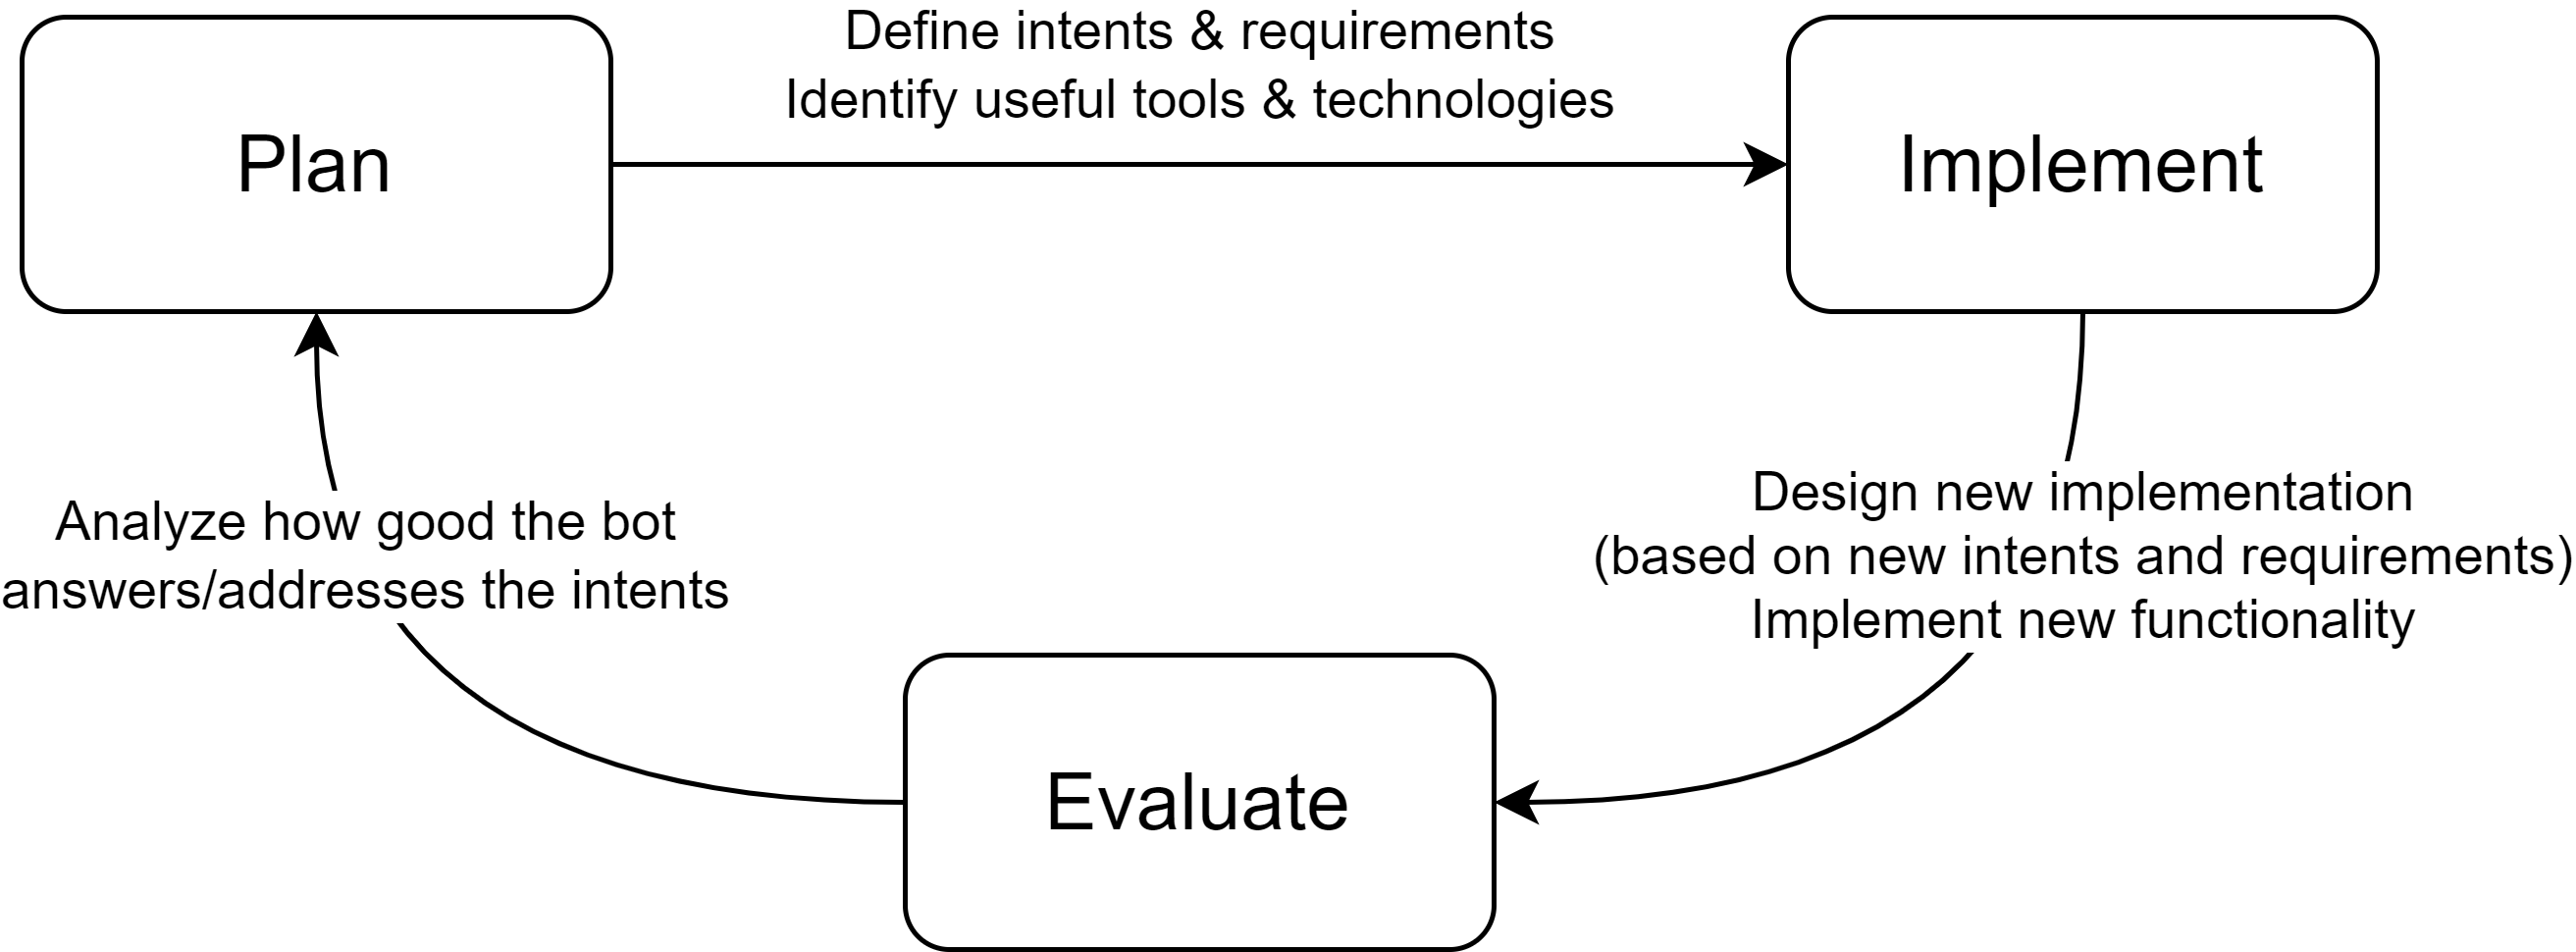
\includegraphics[width=0.8\textwidth]{graphics/iterative-design.png}
\caption{Visualization of the Iterative Development Process}
\label{fig:iterative-design}
\end{figure}
The research methodology for this thesis involves an iterative development process, which is shown in \cref{fig:iterative-design}. This approach includes defining intents and requirements, selecting tools and technologies, implementing a chatbot prototype, and conducting a thorough evaluation. Detailed information on the methodology can be found in \cref{chap:method}.

% todo Result
The thesis employs a strict evaluation methodology, combining quantitative metrics for model performance with qualitative user studies to assess the chatbot's impact on system explainability and user satisfaction.
The  findings indicate that the implemented chatbot enhances the usability and explainability of smart home systems within the Bosch Smart Home environment. Evaluation metrics combining semantic similarity and JSON accuracy demonstrate the chatbot's capability to handle diverse intents such as device control and data analysis tasks effectively. One of our customized models (``shllama3instruct'') emerged as the top performer, achieving a balanced approach between helpful answers and precise \gls{json} function execution to control devices.
However, participants of our study expressed uncertainty about preferring the chatbot over traditional interfaces and challenges remain as our chatbot does not always answer in the same language the user wrote for example.

% Contributions [explicit]
\section{Explicit Contributions}
This thesis advances smart home automation by developing a user-friendly, explainability-enhancing chatbot and providing a practical architecture for integrating large language models into smart home environments without extensive fine-tuning. 
It offers novel insights into chatbot architectures, tools, and methodologies for answering complex questions within smart home systems, particularly the Bosch Smart Home environment. 
While integrating a chatbot into smart homes proves challenging for complex intents, it presents unique opportunities for providing insights otherwise unattainable. 
The research assesses the chatbot's capabilities, addresses potential implementation challenges, and offers recommendations for future developments. 
Ultimately, this work aims to deepen users' understanding of their smart homes, enhancing transparency and usability of home automation systems, contributing valuable knowledge to both academic and industry spheres in the rapidly evolving field of smart home technologies.

\section{Cooperation with Bosch Smart Home}
This thesis is conducted in collaboration with Bosch Smart Home, a leader in home automation technology. Bosch Smart Home, part of the Bosch Group, specializes in innovative solutions to enhance comfort, security, and energy efficiency.
Our partnership focuses on exploring the integration of a chatbot into the Bosch Smart Home system. This cooperation ensures that the research findings are practically relevant and directly applicable and also provides a smart home system to build the chatbot on.

\newpage
\section*{Thesis Structure}
The structure of this thesis is the following:
\begin{description}
    \item[Chapter~\ref{chap:foundation} -- \nameref{chap:foundation}] This chapter lays the groundwork by discussing foundational concepts and reviewing related work in the field of smart home chatbots.
    \item[Chapter~\ref{chap:method} -- \nameref{chap:method}] This chapter outlines the methodology, detailing the iterative process used for developing and refining the chatbot, including expert interviews and user surveys.
    \item[Chapter~\ref{chap:concept} -- \nameref{chap:concept}] This chapter presents the concept for the chatbot, including the definition of intents, architecture design, and requirements gathered from preliminary research.
    \item[Chapter~\ref{chap:implementation} -- \nameref{chap:implementation}] This chapter details the implementation of the chatbot, discussing the technology stack, server and client components, interaction flow, and challenges encountered during development.
    \item[Chapter~\ref{chap:evaluation} -- \nameref{chap:evaluation}] This chapter provides a comprehensive evaluation of the chatbot's performance. It includes the study design, performance metrics, user experience feedback, results of the evaluation, a discussion of the findings, and an analysis of potential threats to validity.
    \item[Chapter~\ref{chap:conclusion} -- \nameref{chap:conclusion}] This chapter concludes the thesis, summarizing findings, discussing the implications, suggesting directions for future research, and reflecting on the limitations and lessons learned.
\end{description}

% !TeX spellcheck = en_US

\chapter{Foundations and Related Work}
\label{chap:ch2}
\label{chap:foundation}

In the exploration of chatbot technology and its applications, this section delves into foundational aspects and related work that form the basis of effective chatbot development. 
The foundations include concepts such as smart homes, chatbot types, and building blocks, providing insights into the underlying principles and methodologies. 
As the foundation is established, the discussion extends to related work, examining existing literature on chatbots in smart homes and their applications in complex scenarios. 
By understanding these foundational elements and existing research, the subsequent sections aim to contribute novel insights and advancements in the field of chatbot development.

\section{Foundations}
\label{sec:foundation}
In this subsection, the focus are the specific foundations that are crucial for the development of chatbots.
Including key elements for this thesis such as a definition for a Smart Home and Natural Language Understanding which enables chatbots to understand a users input message.
Other elements such as a general architecture and typical building blocks for chatbots are also presented.

\subsection*{Smart Home} 
A smart home devices main aspect is that its original functionality is augmented through network capabilities \cite{schiefer_smart_2015,balakrishnan_smart_2018} and should enhance especially comfort\cite{matsui_information_2018, balakrishnan_smart_2018} but also security\cite{balakrishnan_smart_2018} or energy efficiency\cite{matsui_information_2018, balakrishnan_smart_2018} for example. 
Therefore a smart home consists of such devices and provides additional infrastructure like an app to control the devices. 
These infrastructures often allow automation of the devices.
Since its functionality is based on connected devices and often sensors it is often named in the context of the Internet of Things (IoT) \cite{atzori_internet_2010}. 

\subsection*{Chatbot Types and Classifications}
% lehmann
Based on Lehmann \cite{lehmann_chatbot-guide_2021} there are three main types of chatbots: decision-tree-based, keyword-based, and advanced context-aware bots. 
Decision-tree-based bots follow a predefined flowchart in response to user queries, often identified by menus and buttons. 
Keyword-based bots recognize specific keywords, making decisions and providing responses based on internal knowledge. 
Advanced context-aware virtual assistants engage in free-flowing conversations, learning from interactions and offering versatile responses.

% adamopoulou
Additionally, according to Adamopoulou and Moussiades\cite{adamopoulou_overview_2020} chatbots can be classified based on their \textbf{knowledge domain}, with open domain bots discussing general topics and closed domain bots focusing on specific knowledge domains. 
In terms of \textbf{service}, interpersonal chatbots act as information intermediaries, offering communication services like restaurant or flight booking. 
Intrapersonal chatbots, existing within the user's personal domain, function as companions, understanding users like humans. 
Inter-agent chatbots, omnipresent in nature, facilitate inter-chatbot communication. 
\textbf{Goal-based} classification includes informative chatbots providing stored information, chat-based bots conversing like humans, and task-based bots performing specific functions intelligently. 
\textbf{Input processing and response generation} methods vary, from rule-based models relying on predefined rules to retrieval-based models using APIs, and generative models employing machine learning techniques. 
\textbf{Human-aided} chatbots incorporate human computation for flexibility and robustness.
The \textbf{build method} distinguishes between open-source platforms allowing intervention and closed platforms acting as black boxes but providing immediate access to advanced technologies, often found in large companies.

\subsection*{Chatbot Building Blocks}
In this subsection building blocks and architectural insights that can be identified in different literature are collected and explained. 
It is mostly based on Lehmann \cite{lehmann_chatbot-guide_2021} and \cite{adamopoulou_overview_2020} if not mentioned otherwise.

\subsubsection{Natural Language Understanding (NLU) and Machine Learning}
NLU, a subset of Natural Language Processing (NLP), is essential for chatbots.
It involves training algorithms to understand and process natural language, bridging the gap between human language and artificial intelligence. 
NLU is critical for successful chatbot operation, enabling the machine to comprehend user intents and contexts.

Machine learning and NLP also play roles in the evolution of virtual assistants. 
Machine learning algorithms, based on training data, build statistical models and autonomously improve over time.
NLP focuses on processing and understanding natural language, incorporating elements from computer science, AI, linguistics, and data mining. 
These technologies empower chatbots to interpret complex human language, allowing for more sophisticated and context-aware interactions.

\subsubsection{Intents}
Chatbots operate with three key components – Utterances, Intents, and Entities. Intents represent different user intentions that a chatbot anticipates, each consisting of various utterances (training phrases) and one or more responses. Utterances are potential user expressions or example questions, and entities are real-world objects mentioned in a sentence. This structure facilitates the interpretation of natural language, enabling chatbots to recognize user intents and associated entities for effective communication.

Chatbots are built on different intents, each with various utterances and responses. 
The training involves teaching the bot to recognize user intents based on a set of training phrases. 
A Natural Language Processing Engine interprets natural language, transforming it into structured language, and identifies entities within sentences to enhance contextual understanding.

There are also narrow work that regard intent-based chatbots as a separate species \cite{luo_critical_2022}. 
These then typically deal with the technique used to generate responses to ultimately categorize the chatbots.

\subsubsection{Knowledge Bases}
Knowledge bases serve as a crucial component for chatbots, providing them with the necessary information to respond intelligently to user queries. 
These databases store domain-specific data, facts, and contextual information that enable chatbots to understand and address user requests accurately.

\subsubsection{General Chatbot Architecture}
In general, the chatbot architecture by Adamopoulou and Moussiades\cite{adamopoulou_overview_2020} which can be seen in \cref{fig:chatbot-architecture-general} consists of components such as the Language Understanding Component, which interprets user requests and identifies intentions and associated information, and the Dialogue Management Component, which keeps track of the conversation context, processes clarifications, and asks follow-up questions. After understanding the user's request, the chatbot executes actions or retrieves data from its Knowledge Base or external resources, and the Response Generation Component generates natural language responses based on the intent and context information.


\iffalse
\subsubsection{A chatbot taxonomy}
\begin{figure}[h]
\centering
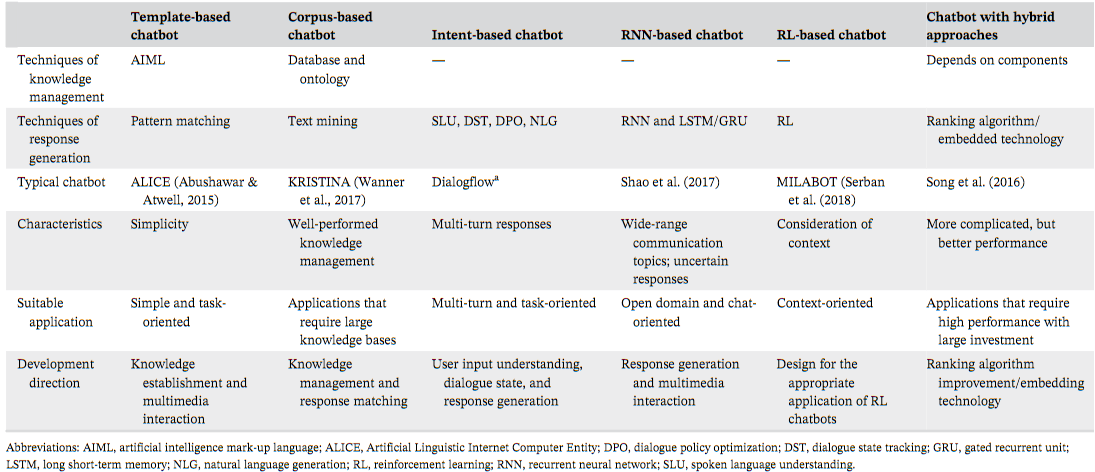
\includegraphics[width=0.98\textwidth]{graphics/chatbot-taxonomy-raymond.png}
\caption{An example taxonomy of chatbots \\Source: Luo et al. \cite{luo_critical_2022}}
\label{fig:chatbot-taxonomy}
\end{figure}
\newpage
\fi


\subsection*{Prototype and Iterative Development}

This subsection is based on Sommerville \cite{sommerville_software_2011} according to who "iterative development of the prototype is essential".
The process for developing a prototype is shown in \cref{fig:prototype-process} and summed up consists of planning, developing and evaluating.
Another iterative process is the extreme programming release cycle which is shown in \cref{fig:extreme-prog-cycle} and consists of user stories that are selected and developed throughout one cycle.
Based on this concepts and needs for our chatbot prototype we built the iterative development cycle that is shown in \cref{fig:iterative-design} which could be seen as a combination of the both processes presented in this subsection.
It is useful to start projects like this thesis with a prototype with thought out case \cite{lehmann_chatbot-guide_2021}.

\begin{figure}[t]
\centering
\captionsetup{justification=centering}
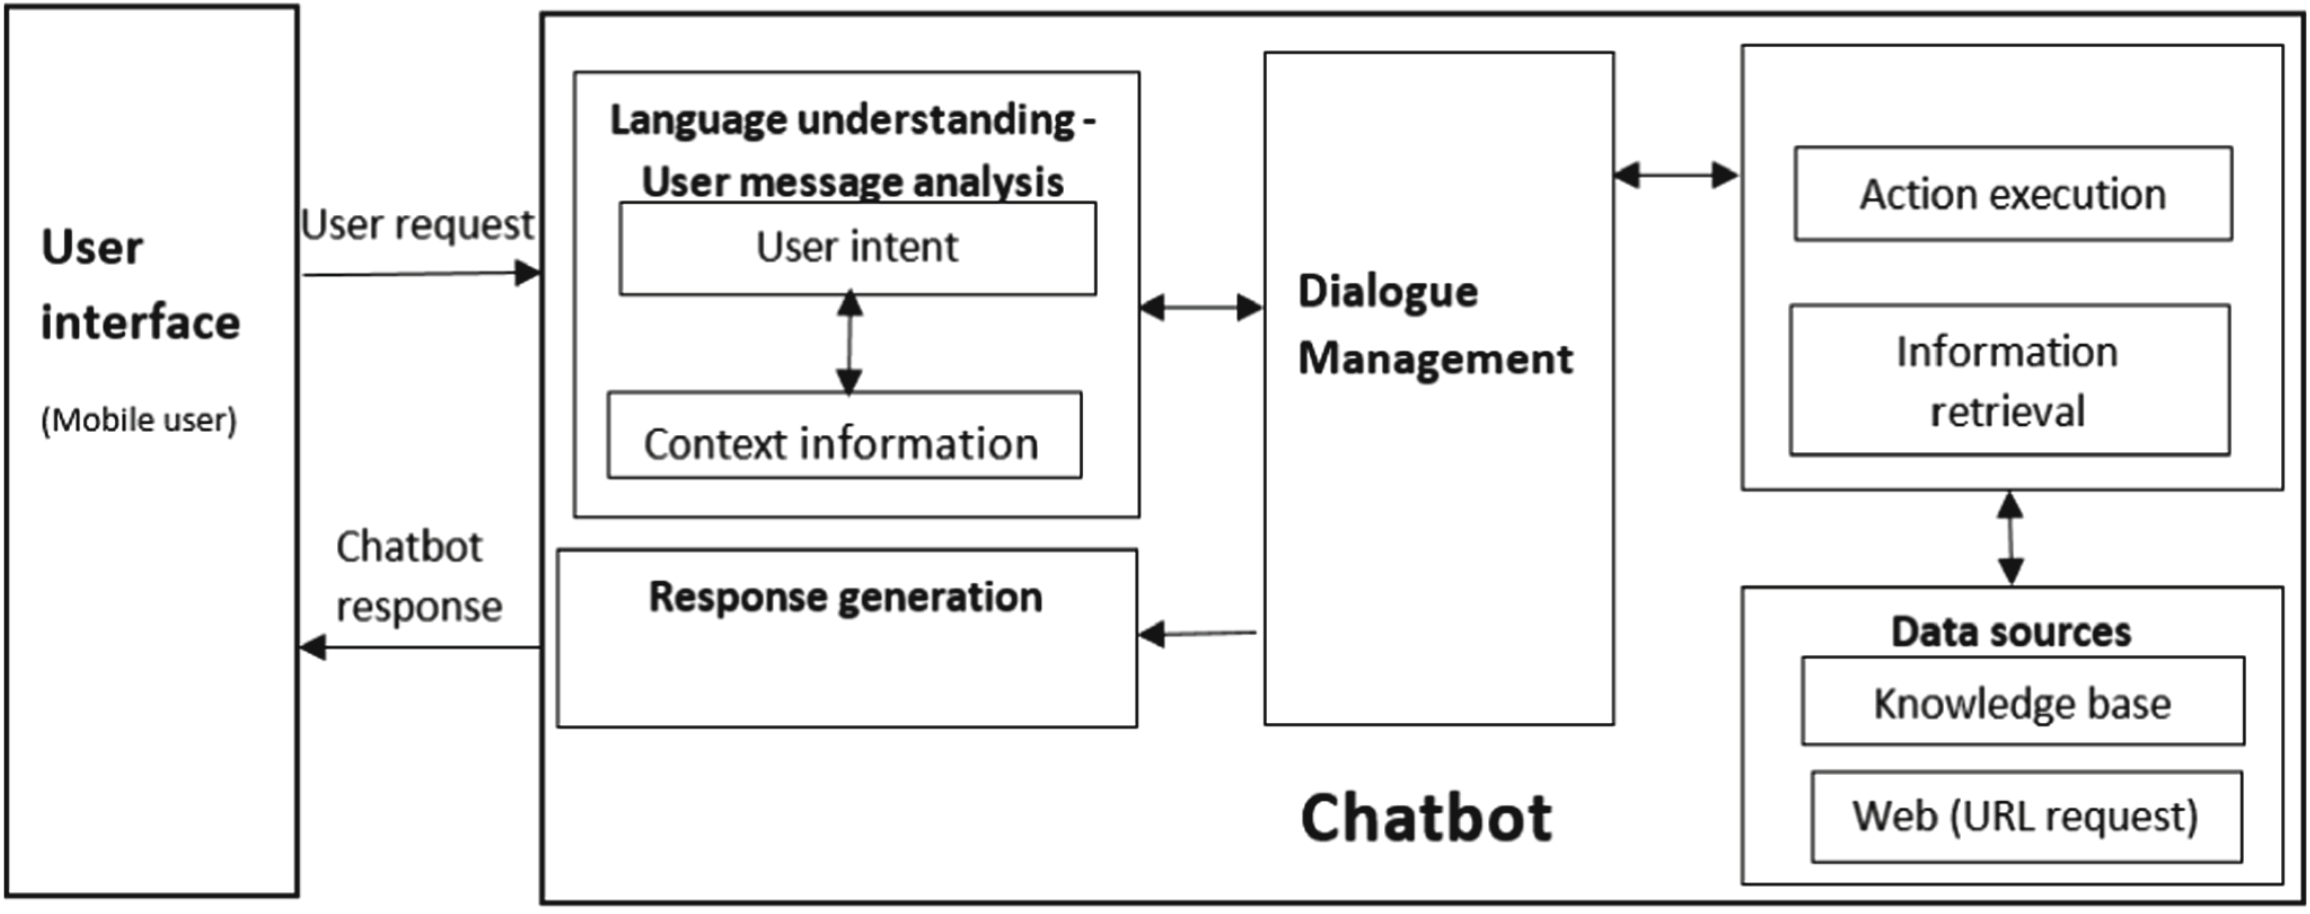
\includegraphics[width=0.98\textwidth]{graphics/chatbot-architecture-general.png}
\caption{An example architecture of chatbots in general \\Source: Adamopoulou and Moussiades \cite{adamopoulou_overview_2020}}
\label{fig:chatbot-architecture-general}
\end{figure}

\begin{figure}[h]
\centering
  \begin{subfigure}{.7\textwidth}
    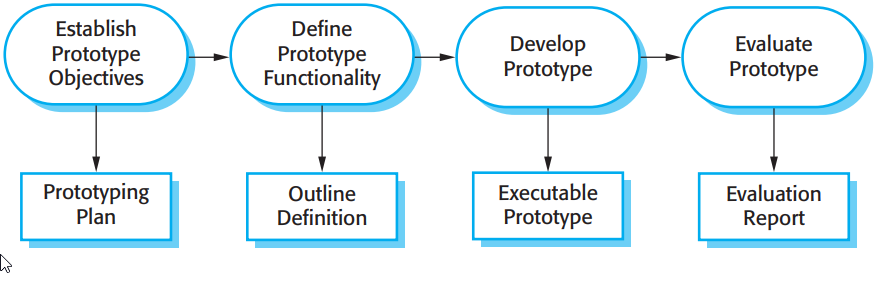
\includegraphics[width=\textwidth]{graphics/prototype-dev.png}
    \caption{Prototype development process}
    \label{fig:prototype-process}
  \end{subfigure} \hfill
  \begin{subfigure}{.63\textwidth}
    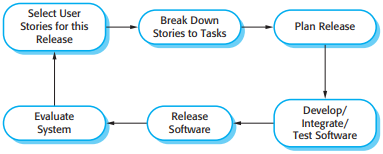
\includegraphics[width=\textwidth]{graphics/extreme-programming-release-cycle.png}
    \caption{Extreme programming release cycle}
    \label{fig:extreme-prog-cycle}
    \end{subfigure}
  \caption{Visualized development processes \\ Source: Sommerville \cite{sommerville_software_2011}}
  \label{fig:dev-processes}
\end{figure}

\newpage
\section{Related work}
In addition to discussing about foundations, you need to discuss about why the problem you are tackling has been insufficiently solved before. To do so, you need to mention related work and discuss what is the difference between your work and those related works.
This section presents literature that is related to this thesis.
While chatbots are ever known to be used in areas like customer service it is interesting to see work on how chatbots are used in smart homes or for complex scenarios like managing containerized networks.
Some literature has the nice side effect that it also presents the architecture of the developed system and can inspire the architecture of the chatbot that should be developed in this thesis.

\subsection*{Chatbots for Smart Homes}
Various literature exists that contains some kind of chatbot in the context of Smart Homes.
Most of these chatbots perform the same task as nowadays common Voice assistants as for example the Google Assistant\footnote{\href{https://assistant.google.com/}{assistant.google.com}} which is capable of understanding written request but also transforming speech into written requests which also includes managing smart devices added to Google Home\footnote{\href{https://home.google.com/intl/de_de/the-latest/}{home.google.com}}, an app for managing a smart home.

Baby et al.\cite{baby_home_2017} presented an approach for a chatbot that can control multiple smart devices in a smart home.
The developed prototype is capable of answering simple questions that regard the devices or change variables of the devices.
It is able to answer questions like "What is the temperature in room 1" or "Set the temperature to 19 degrees celsius".
The architecture includes multiple building blocks that were explained in \cref{sec:foundation}: An NLP Pipeline which in the end identifies the intent of a message and matches an action to.
The pipeline can be seen in \cref{fig:chatbot-pipeline-baby}
The intents and pipeline of this chatbot could inspire the inital iteration of our prototype. 
\begin{figure}[h]
\centering
%\captionsetup{justification=centering}
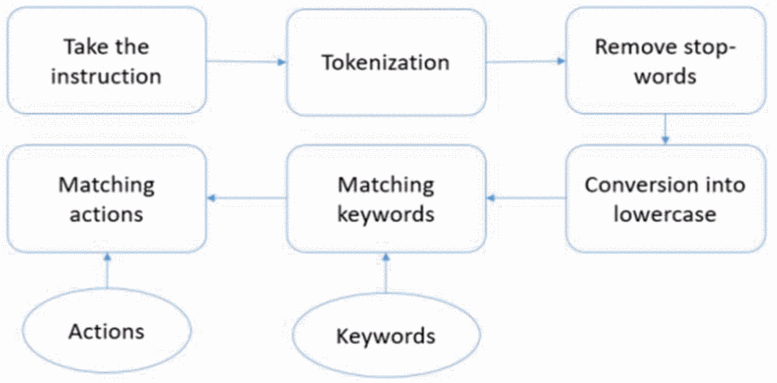
\includegraphics[width=0.66\textwidth]{graphics/baby2017chatbot.png}
\caption{A simple NLP pipeline for a chatbot \\Source: Baby et al. \cite{baby_home_2017}}
\label{fig:chatbot-pipeline-baby}
\end{figure}

Another work developed and connected a chatbot to the facebook (today called meta) messenger for controling smart home devices fans and lights but also gas leakage detection or humidity monitoring \cite{ahmed_smart_2020}.
Intents are not clearly defined or at least not stated but it seems to be a simple decision-tree-based chatbot.
This is probably due to focus of the work laying more in the systems architecture and a limited amount of intents.

A different work explored the area of collaboratively teaching where a focus was set on mitigate malicious activities \cite{chkroun_safe_2021}.
The presented chatbot called Safebot is intended as an extension to smart home assistants and is able to communicate when it does not know the answer the a request and can be taught afterwards.
Also, users could notify the bot that an response was not appropriate resulting in also teaching it.
The learning is purely based on natural languages in contrast to chatbots that for example use knowledge bases with structured data.

\subsection*{Chatbots for complex Scenarios}
Various chatbots for many different use cases exist. 
As the intention of this work is to test how far a chatbot can go in answering complex queries to a smart home the question aligns if approaches exist for answering (complex) questions in a closed domain based on available data.
An example for this is the work of Ait-Mlouk and Jiang \cite{ait-mlouk_kbot_2020} which approached to develop a knowledge graph based chatbot that can find information in linked data through NLU.
The researches in this work address challenges like understanding many different queries (and intents) and making the use of multiple languages and knowledge bases available.
The system developed is able to be extended with new domains.
The architecture of it can be seen in \cref{fig:kbot}.
While it is too complex to explain in detail, it processes queries into intents and entities (through Named Entity Recognition) which in combination make it possible to retrieve information from connected knowledge bases by transforming it into queries and selects a response based on a knowledge graph.

\begin{figure}[h]
\centering
%\captionsetup{justification=centering}
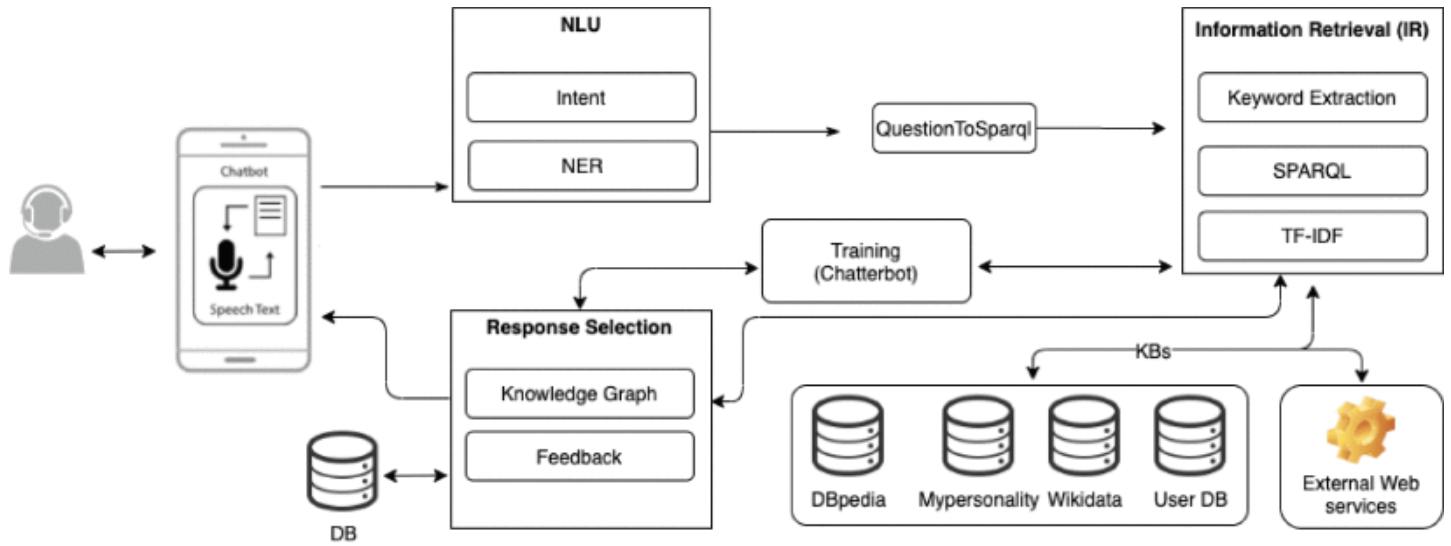
\includegraphics[width=0.94\textwidth]{graphics/KBot-architecture.png}
\caption{Detailed Architecture of KBot \\Source: Ait-Mlouk and Jiang \cite{ait-mlouk_kbot_2020}}
\label{fig:kbot}
\end{figure}

Another research presented a chatbot that can create and manage a containerized network, thus acting as a workflow manager \cite{jasinski_chatbot-based_2023}.
It enables less human involvement by computing requirements written by users.
This leads to a decreasing need for users to have extensive knowledge of the underlying tools to be able to setup such networks and also makes the management of them easier in general.
This can be mapped to this thesis where one aim is to enable even users with less technology knowledge to analyze complex scenarios in their smart home and to make the analysis of those easier in general.

A different work \cite{carlander-reuterfelt_jaicob_2020} approached to develop a chatbot that helps to gain knowledge about Data Science and Machine Learning.
The architecture includes information retrieval from a knowledge base, parsing the received document and answering a query based on the search in the knowledge base.
It also includes a "Small Talk Module" which improves users satisfaction with the system and increase the overall interest in chatting with it.

%noch etwas Fülltext
%\blinddocument

\chapter{Methodology}
\label{chap:method}
This chapter outlines the research methodology employed in this thesis, focusing on the scientific methods used to address the research objectives.

The research methodology of this master's thesis is a comprehensive, mixed-methods approach that incorporates elements of design science and exploratory and empirical research.
This approach is well-suited for a thesis in the field of smart home technologies which are deeply connected with human-computer interaction while we at the same time also take a look at the architecture and building blocks of the intended chatbot.
Due to its structured nature, design science enables an iterative development of the chatbot and the solving of specific problems and therefore is commonly used in software engineering research.
On the other hand the explorative empirical approach aids in understanding user requirements and gathering real-world data to inform the design process and in the end collecting and analyzing evidence that is observable and measurable.

\paragraph{Methods Used:}
%Literature Review including the topics: classification and types of chatbots, typical building blocks used in chatbots, function calling in language models and similar chatbot research, for example smart home chatbots for simple tasks or chatbots for complex scenarios like using multiple knowledge bases, evaluation techniques used for similar language model based chatbots
%iterative
%The chatbot was developed iteratively, as visualized in \cref{fig:iterative-design} of the Introduction chapter. Each iteration involved planning, implementation, testing, and evaluation phases to refine the chatbot's functionality based on performance. Initially, the approach was to add new intents with each iteration. However, the focus shifted to exploring how to develop the first intents effectively and iteratively improving their addressing. This adjustment allowed for a more thorough understanding and enhancement of the initial functionalities.
%preliminary interviews with experts of different domains to gather requirements and ideas for the chatbot development. This qualitative data informed the initial design and development stages.
%survey for gathering example user inputs for the chatbot. Resulting from the preliminary interviews we conducted a survey to gather example user inputs for the chatbots which were essential for developing and also the evaluation
%prototype implementation
%A prototype of the chatbot was designed and implemented within the Bosch Smart Home system, utilizing a client-server architecture. The technology stack included open-source tools to support the development and integration processes.
%study design:
%model performance mostly quantitative but also qualitative analysis of what did work out what did not and why, including the building of an evaluation dataset partly based on the  
%quantitative and qualitative analysis through an experiment: user study with tasks to complete with the chatbot, questionnaire and semi-structured interviews.

A comprehensive literature review was conducted, covering several key areas relevant to chatbot development and smart home technologies. This review explored the classification and types of chatbots, typical building blocks used in their construction, and the emerging technique of function calling in language models. Additionally, similar chatbot research was examined, including studies on smart home chatbots for simple tasks and more complex scenarios involving multiple knowledge bases. The review also investigated evaluation techniques used for language model-based chatbots, providing a solid foundation for the evaluation methodology employed in this study.

The development process followed an iterative approach, as illustrated in \cref{fig:iterative-design} of the Introduction chapter. Initially, the strategy was to introduce new intents with each iteration. However, as the project progressed, the focus shifted towards developing the initial intents more effectively and iteratively improving their implementation. This adjustment enabled a more thorough understanding and enhancement of the core functionalities.

To gather requirements and ideas for the chatbot development, preliminary interviews were conducted with experts from various domains. This qualitative data was instrumental in informing the initial design and development stages, ensuring that the chatbot's features aligned with real-world needs and expectations.

Following the insights gained from the preliminary interviews, a survey was conducted to collect example user inputs for the chatbot. These user inputs were crucial not only for the development process but also for the subsequent evaluation phase. By incorporating real user language and expectations, the chatbot could be designed to better meet user needs and preferences.

A prototype of the chatbot was designed and implemented within the Bosch Smart Home system, utilizing a client-server architecture. The technology stack was carefully selected to include valuable open-source tools.

The evaluation of the chatbot employed a mixed-methods approach, combining quantitative and qualitative analyses. The model performance was assessed primarily through quantitative metrics, but also included a qualitative analysis of successful and unsuccessful outcomes, examining the reasons behind these results. An evaluation dataset was constructed, partly based on the user inputs gathered from the survey, to ensure a comprehensive and realistic assessment of the chatbot's capabilities.

To gain insights into the user experience and overall effectiveness of the chatbot, a user study was conducted. This study comprised a set of tasks for participants to complete using the chatbot, followed by a questionnaire to gather quantitative data on user satisfaction and perceived usability. Additionally, semi-structured interviews were conducted to collect rich, qualitative data on user experiences, preferences, and suggestions for improvement.
% !TeX spellcheck = en_US

\chapter{Concept}
\label{chap:concept}

In this chapter, we describe the intents defined for the smart home system chatbot. These intents aim to provide users with a versatile and intuitive interface for interacting with their smart home devices. The primary focus is on ensuring the chatbot can understand and respond to a wide range of user inputs, offering functionalities that surpass current smart home solutions.

\section{Intent Engineering}

Intents are fundamental to the functionality of the chatbot. Each intent represents a specific user request or command that the system needs to understand and act upon. The design of these intents considers the limitations of existing voice assistants and aims to provide a more flexible and user-friendly experience.

\subsection{Iteration 1: Basic Intents}

\paragraph{Providing Device Status}

\begin{itemize}
    \item \textbf{Intent Name:} GetDeviceStatus
    \item \textbf{Examples:}
    \begin{itemize}
        \item "What is the temperature in the living room?"
        \item "What is the status of the thermostat in the living room?"
        \item "Is it warm in the living room?"
    \end{itemize}
    \item \textbf{Entities:}
    \begin{itemize}
        \item DeviceType (e.g., thermostat, lights)
        \item Room (e.g., living room, bedroom)
    \end{itemize}
    \item \textbf{Action/Response:} Providing information about the specified device in the given room, such as the temperature and power status of a thermostat.
\end{itemize}

This intent aims to provide a more conversational approach to querying device statuses. Unlike existing solutions that require specific device names, our chatbot can understand various formulations, allowing users to ask for the temperature without needing to specify the exact device name or its location.

\paragraph{Changing Device Status}

\begin{itemize}
    \item \textbf{Intent Name:} SetDeviceStatus
    \item \textbf{Examples:}
    \begin{itemize}
        \item "Set the temperature to 22 degrees in the living room."
        \item "Turn off the lights in the bedroom."
        \item "Make it cooler in the kitchen."
    \end{itemize}
    \item \textbf{Entities:}
    \begin{itemize}
        \item DeviceType (e.g., thermostat, lights)
        \item Room (e.g., living room, bedroom)
        \item DesiredStatus (e.g., temperature, on/off state)
        \item DesiredValue (e.g., specific temperature, on/off)
    \end{itemize}
    \item \textbf{Action/Response:} Executing the specified action to set the desired status of the mentioned device in the given room, such as adjusting the temperature for a thermostat or turning lights on or off.
\end{itemize}

This intent enhances user experience by allowing natural language commands to control devices. The chatbot interprets a wider range of user commands, enabling users to control their devices more intuitively and without needing to remember specific device names.

\subsection{Iteration 2: Intermediate Intents}

\paragraph{Assistance for Creating Automations}

\begin{itemize}
    \item \textbf{Intent Name:} CreateAutomation
    \item \textbf{Examples:}
    \begin{itemize}
        \item "Set up an automation for turning off lights at 10 PM."
        \item "Create a rule to adjust thermostat settings when I leave home."
        \item "Can you help me with automating my smart blinds?"
        \item "Notify me if any windows are open."
    \end{itemize}
    \item \textbf{Entities:}
    \begin{itemize}
        \item DeviceType (e.g., lights, thermostat, blinds)
        \item TriggerEvent (e.g., time-based, occupancy, temperature change)
        \item Condition (optional, e.g., specific temperature threshold)
        \item Action (e.g., turn off, adjust settings)
        \item Location (optional, e.g., living room, bedroom)
    \end{itemize}
    \item \textbf{Action/Response:} Assisting the user in defining and setting up a smart home automation, including specifying the devices involved, the triggering event, any conditions, and the desired actions. The chatbot may also provide suggestions for common automation scenarios.
\end{itemize}

Creating automations is a common use case in smart home systems. This intent aims to streamline the process, allowing users to set up complex automations through simple conversational interactions, thus reducing the need for technical knowledge or precise phrasing.

\paragraph{Interpret the Device Control}

\begin{itemize}
    \item \textbf{Intent Name:} DeviceControlInterpretation
    \item \textbf{Examples:}
    \begin{itemize}
        \item "Why did the lights in the bathroom turn on just now?"
        \item "Can you explain the reason for the thermostat adjusting the temperature?"
        \item "What triggered the blinds to open in the living room?"
    \end{itemize}
    \item \textbf{Entities:}
    \begin{itemize}
        \item DeviceType (e.g., lights, thermostat, blinds)
        \item Location (optional, e.g., bathroom, living room)
        \item Action (e.g., turn on, adjust temperature, open)
        \item TriggerSource (e.g., automation, manual activation)
        \item Timestamp (optional, for specifying a time reference)
        \item Reason (optional, e.g., reason for an automation that the user provided when creating it)
    \end{itemize}
    \item \textbf{Action/Response:} Providing an explanation for recent smart home device actions. The chatbot interprets the cause of device events, distinguishing between automation-driven events and those triggered manually by the user. It may also consider time-based context when explaining device actions.
\end{itemize}

This intent addresses a gap in current systems by explaining the reasons behind device actions. It improves transparency and user trust in smart home systems by providing clear explanations for automated and manual device actions.

\subsection{Iteration 3: Complex Intents}

\paragraph{Analyzing Energy Consumption}

\begin{itemize}
    \item \textbf{Intent Name:} AnalyzeEnergyConsumption
    \item \textbf{Examples:}
    \begin{itemize}
        \item "Can you analyze the energy consumption in my home?"
        \item "Provide insights into power usage over the last week."
        \item "How can I optimize energy consumption in the living room?"
    \end{itemize}
    \item \textbf{Entities:}
    \begin{itemize}
        \item AnalysisType (e.g., overall consumption, specific devices)
        \item TimeFrame (e.g., last week, last month)
        \item Room (e.g., living room, kitchen)
    \end{itemize}
    \item \textbf{Action/Response:} Generating a detailed analysis of energy consumption based on the specified parameters. It includes insights into overall energy usage, specific device contributions, and recommendations for optimizing energy consumption in the specified room or timeframe.
\end{itemize}

Energy consumption analysis is a valuable addition to smart home capabilities. This intent provides users with actionable insights into their energy use, helping them to make informed decisions about energy efficiency and cost savings.


%% Auslagern in eigenes chapter??? %%
\section{Preleminary Interviews to Gain Knowledge, Requirements and Ideas}
Preceding to further actions Interviews with a few individuals were conducted to gain knowledge, requirements and ideas for this thesis.
All of the four interviewed were from different domains: One is a researcher and has knowledge in \gls{ai} technologies or more precisely about \glspl{llm} while the three other interviewees are from Bosch.
One of them is working in \qq{AskBosch} but also has expertise in the Smart Home and \gls{iot}. 
The other two are both from Bosch Smart Home where one is a Software Developer and the other a Product Developer.
Therefore a diverse group of interviewees has been formed.

The interview was designed to be open but some guided questions were formulated which were selected based on the domain of the interviewed since not all questions met every present domain.
For example it would have not make sense to ask a Smart Home Software Developer about recent tools or the architecture of \gls{llm}-based applications.
In the following all guided questions are listed:

\begin{enumerate}
    \item \textbf{Feasibility and Key Considerations} \\
    What are your thoughts on the feasibility of a smart home chatbot for providing explainability and enhancing user experience?
    \item \textbf{Interesting Intents}
    From your perspective, what could be interesting intents for a smart home chatbot to address complex user queries?    
    \item \textbf{Selected Intents}
    What is your opinion on the specific intents that have been selected for the chatbot development?    
    \item \textbf{Tools/Technologies/Models}
    In your research experience, what tools, technologies, or models would you recommend for developing a chatbot tailored for smart home applications?
    Would you chose a large language model and input context and user request into it or rather a NLP pipeline that chooses further actions based on the user request?   
    \item \textbf{Data Organization}
    How would you suggest organizing and feeding data to the chatbot, considering the complexity of smart home scenarios?    
    \item \textbf{Common Issues/Pitfalls}
    Based on your expertise, what are the common issues or pitfalls researchers may encounter when developing chatbots for specialized domains like smart homes?
    \item \textbf{Evaluation of Success}
    How would you propose evaluating the success of a smart home chatbot, especially in terms of providing explainability and user-centric interaction? 
    \item \textbf{Data Sources for the Chatbot}
    Can you identify potential sources from which data for the chatbot could be extracted to address user queries about the smart home?
    \item \textbf{Accessibility of Data}
    Do you foresee any challenges or limitations in accessing the identified data sources for the chatbot development?
           
\end{enumerate}

\subsection{Interview Summary}
\label{sec:interview_summary}

The following summary captures the insights and recommendations from these interviews.

\subsection{Feasibility and Key Considerations}

The feasibility of implementing a smart home chatbot was generally supported by all interviewees, albeit with some caveats:

\begin{itemize}
    \item \textbf{Technical Feasibility}: It is crucial to use proven frameworks and consider whether an LLM is necessary or if Named Entity Recognition (NER) would suffice, particularly given budget constraints. LLMs require significant resources, which may be impractical without a robust client-server architecture.
    \item \textbf{User Experience}: The chatbot must simplify user interactions with smart home devices, removing the need for exact device names and understanding user patterns for better automation.
    \item \textbf{Market Viability}: There are concerns about privacy and trust, which affect the acceptance of AI and chatbots in the market.
\end{itemize}

\subsubsection{Interesting and Selected Intents}

The interviewees proposed several useful intents for the chatbot:

\begin{itemize}
    \item \textbf{Device Control}: Activating or deactivating devices, querying the status of doors and windows, and setting temperatures.
    \item \textbf{Automation Assistance}: Simplifying the creation of automations, such as scheduling device operations and explaining device actions.
    \item \textbf{Energy Management}: Providing insights into energy consumption and optimization suggestions.
    \item \textbf{User-Specific Recommendations}: Customizing suggestions based on user behavior and preferences, such as recommending automations for commonly adjusted settings.
\end{itemize}

\subsubsection{Tools, Technologies, and Models}

Several tools and technologies were recommended for developing the chatbot:

\begin{itemize}
    \item \textbf{LLM vs. NER}: While LLMs offer broad capabilities, NER may be sufficient for specific use cases. But a LLm fine-tuned or customized to suit a specific application can also work out great.
    \item \textbf{Frameworks and Platforms}:  Tools like Microsoft Bot Framework\footnote{\url{https://github.com/microsoft/botframework-sdk}}, Conversational Language Understanding\footnote{\url{https://learn.microsoft.com/en-us/azure/ai-services/language-service/conversational-language-understanding/overview}}, Dialogflow\footnote{\url{https://cloud.google.com/dialogflow}}, and LangChain\footnote{\url{https://www.langchain.com/}} were mentioned as tools for different use cases. Except Dialogflow and the Azure Service Conversational Language Understanding they are open source. Potentially a Spring Boot\footnote{\url{https://spring.io/}} or Node.js\footnote{\url{https://nodejs.org/}} application could suit the use case of this thesis.
    \item \textbf{Data Management}: Organizing data with configurations that map intents to actions, and ensuring the chatbot can correctly interpret inputs is vital.
\end{itemize}

\subsubsection{Data Organization and Sources}

Effective data organization and source identification are a key aspect for achieving the desired chatbot functionality:

\begin{itemize}
    \item \textbf{Configurations and Scenarios}: Initial iterations should use predefined configurations, mapping intents to device actions.
    \item \textbf{Data Collection}: Gathering diverse user inputs to train models and create accurate annotations is essential for generalizability. They are also useful for the evaluation of the performance of the chatbot
    \item \textbf{Potential Sources}: Logs from smart home devices , external services, and user behavior data should be considered. For the beginning the most important data is about the devices of a user since it is crucial for all of the defined intents and the most essential part of a smart home.
\end{itemize}

\subsubsection{Common Issues and Pitfalls}

While the initial intention was to find out about general issues and pitfalls that often occur in the development of chatbot-powered applications in the interviews the direction 
Several potential challenges were highlighted:

\begin{itemize}
    \item \textbf{Complexity of Automations}: Creating sophisticated automations might be challenging and require a balance between simplicity and functionality.
    \item \textbf{Data Privacy and Trust}: Addressing user concerns about privacy and the reliability of AI-generated information is crucial.
    \item \textbf{Resource Constraints}: Ensuring sufficient computational resources for LLMs, if used, and managing the cost of development.
\end{itemize}

\subsubsection{Evaluation of Success}

The success of the smart home chatbot can be evaluated through:

\begin{itemize}
    \item \textbf{Performance Metrics}: Comparing expected outcomes with actual results using metrics like the F1 score.
    \item \textbf{User Experience}: Conducting user evaluations to assess satisfaction and the effectiveness of interactions.
    \item \textbf{Prototyping and Testing}: Iterative testing with real users to refine the chatbot's capabilities and ensure it meets user needs.
\end{itemize}

\subsection{Conclusion}

The interviews provided a comprehensive understanding of the requirements and considerations for developing a smart home system chatbot. Key insights include the importance of choosing the right technologies, ensuring robust data management, and addressing user privacy concerns. By focusing on practical intents and leveraging existing frameworks, the development of a user-friendly and effective smart home chatbot is achievable.


\section{Requirements of the Chatbot}

This section outlines the functional and non-functional requirements of the chatbot designed for integration with smart home systems, particularly focusing on the Bosch Smart Home system.
They are formulated in a general way and not from the view of a specific role.
The requirements were gathered primarily by drawing conclusions from the preliminary interviews.

To shortly discuss requirement types it is well known that  software requirements can be classified into two categories: \glspl{fr} and \glspl{nfr}. 
A common ground is that \glspl{fr} describe what the system shall do (describe specific behaviors and capabilities of the system) where in contrast \glspl{nfr} describe how a system shall do something (focus on quality attributes, constraints, and overall system characteristics).
But in practice, researchers unveiled that it is hard to draw a line between these two types of requirements. \glspl{nfr} often stay very vague and are therefore hard to analyze \cite{nfr_fr}.
But because it is still the most widespread definitions, it is applied in this work.

The following requirements provide a comprehensive foundation for developing a smart home chatbot that is functional, secure, and user-friendly. The focus on integrability with existing systems, particularly the Bosch Smart Home system, ensures practical applicability, while attention to maintainability and cost-effectiveness supports sustainable deployment.

\subsection{Functional Requirements}

\begin{itemize}
    \item \textbf{Intent Addressing}: The chatbot should accurately address the defined intents. The extent of this capability depends on the progress made by the deadline of this thesis.
    
    \item \textbf{Language Support}: The chatbot should support both German and English languages. It should respond in the same language as the user's input. For example, if a user query is in German, the chatbot should reply in German, and likewise for English.
    
    \item \textbf{Integrability}: The chatbot should be easily integrable into existing smart home systems, particularly the Bosch Smart Home system. Integration should require only a mapper class/code capable of splitting the chatbot's output into the natural language response for the user and a system output (a JSON in this work) that maps to the smart home system's functionalities.
    
    \item \textbf{Context Awareness}: The chatbot should maintain context within a session to handle follow-up questions and commands effectively, providing a more natural interaction experience.
    
    \item \textbf{Command Execution}: The chatbot should be capable of executing specific commands related to smart home functionalities, such as turning devices on or off, adjusting settings, and providing status updates.
    
    \item \textbf{Error Handling}: The chatbot should be able to handle errors gracefully, providing helpful feedback to users when it cannot understand a request or when an action cannot be completed.
\end{itemize}

\subsection{Non-Functional Requirements}

\begin{itemize}
    \item \textbf{Security and Safety}: The chatbot may handle sensitive data, including information about users' devices and smart home system logs. It is crucial to ensure this information is not exposed to unauthorized parties. Self-hosting the LLM could enhance security.
    
    \item \textbf{Cost-Effectiveness}: The solution should be cost-effective since LLM-based software can get expensive easily. Self-hosting the LLM could reduce costs associated with third-party services.
    
    \item \textbf{Usability}: The chatbot should be user-friendly, providing clear and concise responses. The interface should be intuitive for users with varying levels of technical expertise. 
    
    \item \textbf{Performance}: While performance is not the primary focus for this proof of concept, the chatbot should respond within a reasonable time to avoid negatively impacting usability. Quick response times are essential for maintaining a smooth user experience.
        
    \item \textbf{Maintainability}: The chatbot system should be easy to maintain and update. Clear documentation and modular design can facilitate easier maintenance and the addition of new features which is always nice to have but also necessary for the Iterative approach of this thesis.
\end{itemize}

\section{Protoype Design and Architecture}
In this section, we outline the design and architecture of the smart home chatbot prototype. This prototype aims to facilitate seamless and intuitive interactions between users and their smart home devices by leveraging advanced natural language processing (NLP) techniques and smart home integration capabilities.

\subsection{Overview}

The smart home chatbot prototype consists of several key components, each playing a vital role in the system's overall functionality. These components include the NLP engine, the intent processing module, the smart home integration layer, and the user interface. Together, they form a cohesive system capable of understanding and executing user commands within a smart home environment.

\subsection{System Architecture}

The architecture of the smart home chatbot prototype is designed to be modular and scalable, ensuring ease of maintenance and future enhancements. The system is divided into the following main modules:

\begin{itemize}
\item \textbf{Natural Language Processing (NLP) Engine}
\item \textbf{Intent Processing Module}
\item \textbf{Smart Home Integration Layer}
\item \textbf{User Interface (UI)}
\item \textbf{Data Management and Storage}
\end{itemize}

\begin{figure}[h]
\centering
\includegraphics[width=0.8\textwidth]{smart_home_chatbot_architecture.png}
\caption{High-Level Architecture of the Smart Home Chatbot Prototype}
\label{fig
}
\end{figure}

\subsubsection{Natural Language Processing}

The NLP engine is responsible for interpreting user inputs and converting them into structured data that the system can process. It employs a large language model (LLM) or Named Entity Recognition (NER) techniques, depending on the complexity and requirements of the task. The NLP engine comprises the following components:

\begin{itemize}
\item \textbf{Preprocessing}: Handles tokenization, stemming, and stop-word removal to prepare user inputs for analysis.
\item \textbf{Intent Recognition}: Identifies the user's intent from the input text.
\item \textbf{Entity Extraction}: Extracts relevant entities such as device types, room names, desired states, and values from the input.
\end{itemize}


\subsubsection{Smart Home Integration Layer}

The smart home integration layer bridges the chatbot and the smart home devices. It translates the processed intents into actionable commands for the smart home system.

\subsubsection{User Interface (UI)}

The user interface is the front-end component that interacts with users. It can be a mobile app, web interface, or integrated into existing smart home apps. The UI is designed to be user-friendly, supporting both German and English languages, and includes:

\begin{itemize}
\item \textbf{Chat Interface}: Allows users to input their queries and receive responses from the chatbot.
\item \textbf{Voice Interface (optional)}: Supports voice commands for hands-free operation.
\item \textbf{Feedback Mechanism}: Enables users to provide feedback on the chatbot's performance, helping to refine and improve the system.
\end{itemize}

\subsubsection{Data Management}

Effective data management is crucial for the chatbot's performance and reliability. This component handles the storage and retrieval of user data, device logs, and conversation histories. It includes:

\begin{itemize}
\item \textbf{Database}: Stores device information, user preferences, and conversation logs.
\item \textbf{Data Privacy Controls}: Implements measures to ensure that user data is handled in compliance with privacy regulations.
\item \textbf{Analytics Engine}: Analyzes user interactions and device data to provide insights and optimize the chatbot's performance.
\end{itemize}

\subsection{Integration with Bosch Smart Home System}

\subsection{Challenges and Considerations}

Several challenges and considerations were addressed during the design and development of the prototype:

\begin{itemize}
\item \textbf{Complexity of Automations}: Balancing simplicity and functionality in user-defined automations.
\item \textbf{Multilingual Support}: Providing accurate and contextually appropriate responses in both German and English.
\end{itemize}


%\section{further parts of the prototype - NLP Pipeline, Integration into the Bosch SH App,...}

%\blinddocument

% !TeX spellcheck = en_US
\chapter{Implementation}
This chapter details the technical realization of the Smart Home Chatbot system, translating the conceptual framework into a functional application. We begin with an overview of our technology stack, which combines Android Studio for client-side development and Ollama for server-side language model hosting.

The chapter is structured to distinctly cover both server-side and client-side components. For the server, we explore the setup process, challenges faced, and model customization techniques. On the client side, we delve into the Android application's development, covering data management within the Bosch Smart Home ecosystem, user interface design, and message handling.

We then illustrate the interaction flow between user, client, and server, demonstrating how these components collaborate to process queries and generate responses. The chapter concludes by addressing key challenges encountered during development, such as multilingual support and historical data limitations, along with their implemented or proposed solutions.

This comprehensive overview provides readers with a thorough understanding of the system's technical architecture and the rationale behind critical design decisions.

\label{chap:implementation}

\section{Technology Stack}
The implementation of the chatbot system leverages a diverse set of technologies, each chosen for its specific capabilities and compatibility with the existing Bosch Smart Home ecosystem. Figure \ref{fig:techstack} illustrates the technology stack overlaid on the base architecture.

Android Studio\footnote{\url{https://developer.android.com/studio}} serves as the primary integrated development environment, facilitating the extension of the existing Bosch Smart Home Android application. The client-side development utilizes Java\footnote{\url{https://www.java.com/}} programming language in conjunction with Android 14 SDK\footnote{\url{https://developer.android.com/about/versions/14}}, ensuring compatibility with the latest Android features and optimizations.

To enhance the user interface and manage the chat functionality efficiently, the implementation incorporates modern Android components. RecyclerView is employed for rendering the message exchange between the user and the chatbot, providing smooth scrolling and efficient memory usage. Concurrency tools, specifically ExecutorService and CompletableFuture, are utilized to handle API calls in the background, ensuring a responsive user interface while managing asynchronous operations.

On the server side, Ollama v0.1.47\footnote{\url{https://ollama.com/}} is deployed for hosting, customizing, and invoking the language model. The Ollama API facilitates seamless interaction between the client application and the server-hosted language model.

\gls{json}\footnote{\url{https://www.json.org/}} serves as the primary data exchange format between the server and client components. This lightweight and human-readable format is used both for constructing API calls to the Ollama API and for transmitting the language model's responses back to the client.
\begin{figure}[h]
    \centering
    \captionsetup{justification=centering}
    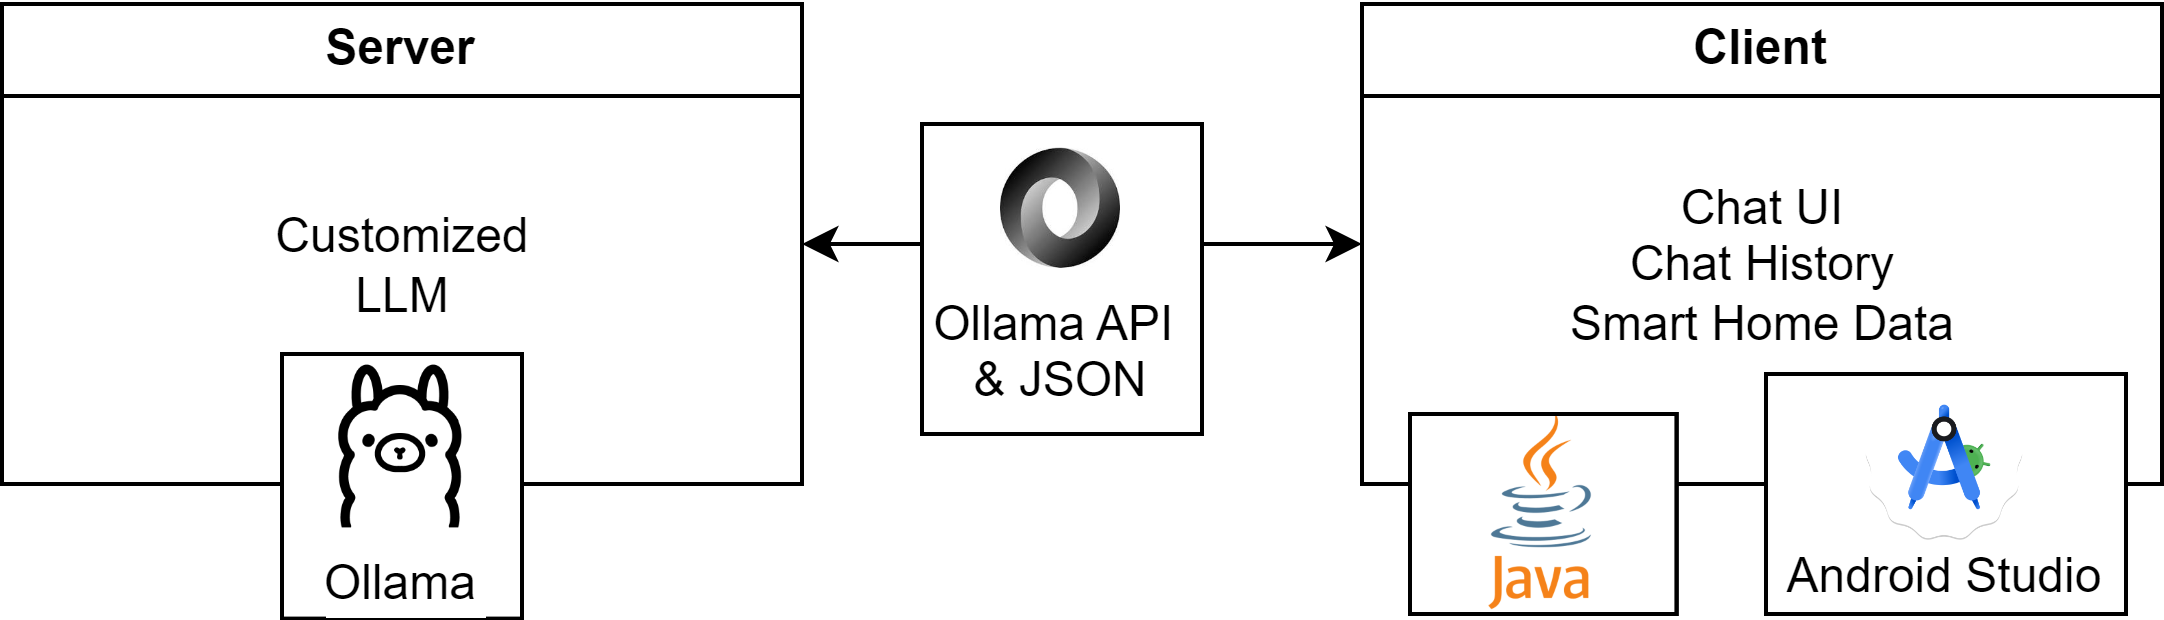
\includegraphics[width=0.9\textwidth]{graphics/techstack.png}
    \caption{Technology stack visualized on base architecture}
    \label{fig:techstack}
\end{figure}

\section{Server}
This section covers the server-side implementation of the Smart Home Chatbot system. 
It details the initial plan to use bwCloud and the challenges that led to switching to a private computer setup. 
We discuss the hardware specifications of the server and how it affects model performance and response times. 
The section also explains the deployment of Ollama v0.1.47 for hosting and customizing language models. 
We then dive into the process of model selection, considering factors like parameter count, popularity, and language support. 
Finally, we explore the techniques used for model customization, including the creation of modelfiles and prompt engineering, to tailor the language models for smart home interactions.

\subsection{Hardware and Performance}
\label{subsec:hardware}
The initial plan was to use the bwCloud\footnote{\url{https://www.bw-cloud.org/}}, a currently free service that can be used of students and researchers of different institutions accross Baden-Württemberg, Germany.
It was easy to get the needed ressources for this project which where eigth VCPUs, 16GB RAM and also enough memory for the size of the \glspl{llm} that were planned to use.
When trying out to run models directly on the server the response times were okay for models up to approximately 10 Billion perameters although the used server has no GPU.
However, when testing customized models through HTTP Requests the response times were much higher than expected.
Especially the first response often took over one minute with preceeding requests taking minimum 30 seconds depending on the length of the generated respone.
The first request usually takes longer when the model used is not allready loaded into the RAM.

Because of the occuring difficulties and with wanting to use as low budget as possible we decided to use an existing private Computer with more Ressources and used IPv6 Host Exposure for a specific port on which the Ollama API was running.
The computer had an NVIDIA GeForce 980 ti graphics card with 6GB VRAM and 32GB RAM with 3600MHz.
Even longer model responses usually only took a few seconds to receive.

\subsection{Model Customization}
\label{subsec:modelcust}
This section is all about the language models themselves. It covers which model where selected and why, how the models where customized with so called ``Modelfiles'' and an engineered prompt.
\subsubsection{Model Selection}
Initially the model in the focus of this work was llama3 since it was one of the most recent models and seen everywhere when starting with the .
However, it makes sense to try out other models and see how they perform therfore we came up with a solid model selection.
The model selection was based on parameter count, popularity, ranking in the \gls{bfcl} and availability in the ollama models library.
Another condition for the model was to support German.
The parameter count should be lower than 15 Billion since it wouldn't really run on the server setup described in the last section.
The model should be either under the most popular models filter on the Ollama library website \footnote{\url{https://ollama.com/library?sort=popular}}

% Define a new column type 'Y' for wider last column
\newcolumntype{Y}{>{\hsize=1.2\hsize}X}
\begin{table}[h!]
    \centering
    \begin{tabularx}{\textwidth}{lXXp{3cm}Xl}
    \toprule
    Model & Parameters & Size & Popularity \newline (Ollama) & BFCL \newline Accuracy & Organization \\
    \midrule
    home-3b-v3 & 3b & 1.7GB & 2.3K & - & - \\
    qwen2-7b-instruct & 7b & 4.4GB & 281.6K & - & Alibaba \\
    qwen2-1.5b-instruct & 1.5b & 0.9GB & 281.6K & - & Alibaba \\
    mistral-7b-instruct & 7b & 4.1GB & 2.8M & - & Mistral AI \\
    gemma-2b-instruct & 2b & 1.7GB & 3.9M & - & Google \\
    gemma-instruct & 7b & 5GB & 3.9M & 43.82 & Google \\
    zephyr & 7b & 4.1GB & 107.8K & - & Mistral AI \\
    llama3 & 8b & 4.7GB & 4.5M & - & Meta \\
    llama3-instruct & 8b & 4.7GB & 4.5M & 60.29 & Meta \\
    phi2 & 2.7b & 1.6GB & 200.1K & - & Microsoft \\
    phi3-3.8b & 3.8b & 2.2GB & 2.1M & - & Microsoft \\
    phi3-14b & 14b & 7.9GB & 2.1M & - & Microsoft \\
    gemma2 & 9b & 5.4GB & 290.1K & - & Google \\
    gorilla-openfunctions-v2 & 6.9b & 2.7GB & <1K & 84.65 & Gorilla LLM \\
    \bottomrule
    \end{tabularx}
    \caption{Overview of the models used.}
\end{table}

Here are some additional notes to this table:
\begin{itemize}
    \item The model \textit{home-3b-v3} was selected because it was fine-tuned to control devices with Home Assistant \cite{acon96_home_llm}.
    \item Only the commercial models from \textit{Mistral AI} are on the BCFL.
    \item \textit{Gemma2} and \textit{Phi3} were released later in the thesis phase, so \textit{gemma} and \textit{phi2} were also used.
    \item We noticed that the \textit{instruct} version of \textit{llama3} performed slightly better for our task than the plain version. Therefore, we usually preferred the instruct versions of other models if available.
    \item The model \textit{gorilla-openfunctions-v2} was not added to Ollama by Gorilla LLM but by a user who made it executable on Ollama.
    \item The \gls{bfcl} accuracy rating is according to the following date: 2024-07-06
    \item The popularity in the Ollama library is based on the amount of pulls of a model. It is one count per model which includes each different version of the model (e.g. instruct, different sizes).
\end{itemize}

\subsubsection{Modelfiles}
Modelfiles are configuration files used to customize and fine-tune language models for specific applications. They allow developers to define instructions, examples, and parameters that guide the model's behavior, ensuring more accurate and contextually appropriate responses. In the context of this project, modelfiles were crucial for tailoring the language model to understand and interact with the Bosch Smart Home system effectively.
The Ollama software uses modelfiles to create and share models. Let's examine the key components of our custom modelfile for the Bosch Smart Home chatbot:

\begin{Listing}
\begin{lstlisting}[language=bash]
FROM llama3:instruct
PARAMETER temperature 0.95
\end{lstlisting}
\caption{Base Model and Temperature Setting}
\label{lst:base_model}
\end{Listing}

The section in \cref{lst:base_model} specifies the base model (llama3:instruct) and sets the temperature parameter. As shown in this listing, the temperature value of 0.95 allows for more creative responses while maintaining coherence.

\begin{Listing}
\begin{lstlisting}[language=bash]
SYSTEM """
You are 'SHBot' (Smart Home Bot), a helpful AI Assistant that controls smart home devices. Complete tasks or answer questions based on a provided device list. Always respond in the language of the user request and keep answers brief.
Answer in the following format containing a natural language response to the user and a json:
natural language answer to the user
{
'action': 'intent/action',
'value': 'optional value for an action',
'deviceID': 'ID of the device',
'device': 'device type',
'room': 'device room',
'name': 'device name'
}
Important: Always place the json at the end of your response.
"""
\end{lstlisting}
\caption{System Message - Part 1: Role Definition and Response Format}
\label{lst:system_message_1}
\end{Listing}

Listing \ref{lst:system_message_1} shows the first part of the system message, which defines the bot's role and sets the expected response format. It instructs the model to provide both a natural language answer and a structured JSON output, which is crucial for integrating the chatbot's responses with the smart home system.

\begin{Listing}
\begin{lstlisting}[language=bash]
SYSTEM """
Available Actions:
'none'
'turn-on'
'turn-off'
'change-temperature(value needed)'
Devices:
'socket': can use 'turn-on' and 'turn-off'
'thermostat' or 'RADIATOR_THERMOSTAT': The measured temperature can be viewed on each individual thermostat (RADIATOR_THERMOSTAT). It is typically structured like this: "id": "TemperatureLevel", "state": { "temperature": 22.5 }
'room-climate-control': can use 'change-temperature(value)'. This is a virtual device in the smart home that manages the temperature (called setPointTemperature) of the thermostats in the same room. If no thermostat exists, the system won't create a room climate control.
'door-window-contact': can't use the actions, only provides information whether its opened or closed.
"""
\end{lstlisting}
\caption{System Message - Part 2: Available Actions and Device Types}
\label{lst:system_message_2}
\end{Listing}

Listing \ref{lst:system_message_2} outlines the available actions and device types in the Bosch Smart Home system. This section provides the model with crucial information about the capabilities and limitations of each device type, enabling more accurate responses to user queries.

\begin{Listing}
\begin{lstlisting}[language=bash]
SYSTEM """
Example conversations:
For this example assume the user has the following devices:
'[{"type": "POWER_METER_SWITCH", "name": "TV", "deviceID": "device123", "state": [{"id": "PowerSwitch", "state": {"switchState": "OFF"}}], "room": "Schlafzimmer"}, {"type": "SHUTTER_CONTACT", "name": "WindowSensor-67890", "deviceID": "device456", "state": [{"id": "ShutterContact", "state": {"value": "CLOSED"}}], "room": "Wohnzimmer"}]'

MESSAGE user Can you turn on my TV?
MESSAGE assistant Sure, turning on the TV now. { "action": "turn-on", "deviceID": "device123", "device": "POWER_METER_SWITCH", "room": "Schlafzimmer", "name": "TV" }
MESSAGE user Sind alle Fenster geschlossen?
MESSAGE assistant Ja, alle Fenster sind geschlossen.
"""
\end{lstlisting}
\caption{Example Conversations and Device List}
\label{lst:example_conversations}
\end{Listing}

Listing \ref{lst:example_conversations} provides example conversations to guide the model's responses. It includes a sample device list and demonstrates how the model should interpret user queries and format its responses, including the use of different languages and the structured JSON output.

\paragraph{Using Example User Inputs for the Modelfiles} 
A significant aspect of our model customization process involved leveraging the example user inputs collected during our survey mentioned in \cref{sec:collectinputs}. We carefully selected a subset of these inputs to include in the modelfile used for customizing the selected \glspl{llm}. This approach allowed us to fine-tune the models with real-world, domain-specific examples, enhancing their ability to understand and respond to typical smart home queries. By incorporating these authentic user inputs into the model's training data, we aimed to improve its contextual understanding and response accuracy for smart home-related interactions and therefore create a more domain-specfic model.

By incorporating these detailed instructions and examples, as shown in Listings \ref{lst:base_model} through \ref{lst:example_conversations}, the modelfile ensures that the language model can effectively understand and respond to user queries about their Bosch Smart Home devices, providing accurate information and executing commands as needed.


\subsubsection{Prompt Engineering}

Prompt engineering is the process of designing and refining input prompts to elicit desired responses from language models. It involves crafting specific instructions, context, and examples to guide the model's output effectively. In the context of our Bosch Smart Home chatbot, prompt engineering was crucial for ensuring accurate and relevant responses to user queries about their smart home devices.

The process of building the prompt is closely intertwined with the development of the modelfile. In our modelfile, we defined how the model should act and specified that it would be provided with a device list for each user. This integration of prompt engineering and modelfile development was essential for creating a cohesive and effective chatbot system.

Several approaches were considered for implementing the prompt engineering:

\begin{enumerate}
    \item \textbf{Utilizing context data:} Some recent models can handle additional context data alongside the user prompt. This would allow for the device list and other relevant information to be provided through this mechanism.

    \item \textbf{Dynamic SYSTEM message updates:} This approach involves changing the SYSTEM message dynamically with each user's device list.

    \item \textbf{Incorporating the device list in the user message:}
    \begin{enumerate}
        \item Building a message history where the first message always contains the current device list, followed by the user's actual message.
        \item Combining the device list and user message in a single prompt, formatted as ``devices: $<>$, message:$<>$''.
        \item Extending the previous approach with a ``mode'' parameter, alternating between ``get-data'' and ``answer-user'' modes based on whether the model has sufficient information to respond.
    \end{enumerate}
\end{enumerate}

Due to our objective of testing different models, the first option of using context data was not suitable, as it would limit our flexibility in model selection.

The ``mode'' approach showed promise in initial tests but proved complex to implement fully. Determining when to switch between modes and managing background calls to the model when it needed more data presented significant challenges.

Dynamically changing the SYSTEM message for each interaction was considered inefficient due to the overhead of updating and sending the entire message via API for every request. We briefly considered implementing a server-side function to update the modelfile with the device list, but ultimately chose a different method.

The final approach we adopted was building a message history. This method proved to be intuitive and straightforward to implement on the client side. By including the device list as the first message in the history, followed by the user's actual query, we could provide the necessary context to the model without overly complicating the implementation or limiting our ability to test different models.

This approach allowed us to maintain flexibility in our model selection while effectively providing the necessary context for accurate responses to user queries about their Bosch Smart Home devices.


\section{Client}
This section provides details about all the components at the client-side as approached in \cref{sec:design}. 
The client-side implementation is a crucial part of the Smart Home Chatbot system, handling user interactions, data management, and communication with the server. It extends the existing Bosch Smart Home Android app, integrating new functionalities while maintaining consistency with the app's design and user experience. 
The following subsections break down the various aspects of the client implementation, including how data is managed, the user interface design, message handling, request construction, and response processing. 
Each component plays a vital role in creating a seamless and efficient chatbot experience for smart home users.

\subsection{Data Management}
Additionally to the \gls{json} data exchange between client and server the data of the smart home itself has to be managed in order to put it into the \gls{json} and transmit it and also handle the \gls{json} received from the server.
The Bosch Smart Home app has an internal data model to store the current state of the users smart home. It updates this model when starting the app and on certain events.
Therefore, two options were available for managing the device data: either using the available data model or sending requests through the available internal API of the system.
To keep the latency low we deviced to use the internal data model and filter relevant data out. As described in \cref{subsec:devices} three devices were considered for the prototype.
Therefore we only used data relevant for the user from this devices. Since there was much unnecessary data in each device state we collected only the data described in \cref{tab:device_state_data_detailed}
\begin{table}[h!]
    \centering
    \begin{tabularx}{\textwidth}{|p{3cm}|X|}
    \hline
    \textbf{Device Type} & \textbf{Collected State Data} \\ \hline
    Smart Plug & 
    \textbf{powerConsumption}: Current power usage in watts \newline
    \textbf{energyConsumption}: Total energy consumed over time in kilowatt-hours \newline
    \textbf{switchState}: Whether the device is turned ON or OFF \\ \hline
    Thermostat & 
    \textbf{valvePosition}: Position of the radiator valve \newline
    \textbf{childLock}: Whether the child lock is ON or OFF \newline
    \textbf{temperature}: Current temperature measured by the thermostat in Celsius \\ \hline
    Room Climate Control & 
    This is not a real device. It is virtually managing all thermostats in one room to achieve a desired temperature.
    \textbf{ventilationMode}: Whether ventilation mode is active. \newline
    \textbf{boostMode}: Whether boost mode is active. This mode is used to increase the heat output for a short time \newline
    \textbf{operationMode}: Current operation mode (automatic or manual) \newline
    \textbf{setpointTemperature}: Desired temperature set by the user in Celsius \newline
    \textbf{currentTemperature}: Actual room temperature in Celsius \\ \hline
    Door Window Contact & 
    \textbf{contactState}: Whether the window or door is OPEN or CLOSED \\ \hline
    \end{tabularx}
    \caption{Detailed state data collected from different smart home devices}
    \label{tab:device_state_data_detailed}
\end{table}

Of course when controling devices the data model has to be updated in parallel to updating the devices themselves.

Another point for data management are the system logs of the Bosch Smart Home system to for example reason why something happened in the system and data from external sources to for example analyze how the electricity price changed.
Since we were not able to implement this it is mentioned in \cref{sec:challenges-solutions}.


\subsection{User Interface}
\label{sec:ui}
% in the main activity in the Bosch Smart Home app multiple views can be selected in the bottom like "Favourites" and "Room". The Toolbar in the top is always shown while in the main activity. Extending this existing functionality we added a button saying "CHATBOT" to the toolbar which can be seen in \cref{fig:ui-homescreen} to have the chatbot functionality available no matter where you are currently in the main activity. This provides a simple but efficient way to get to the chatbot.
% In \cref{fig:chatactivity} an overview of the actual chatbot \gls{ui} is shown. The toolbar here consists of an "Up Button" how it is often called in Android which is just a button to get back to the main activity. It also has an heading "Smart Home Chatbot".
% Directly under the toolbar another bar is shown which is more of an development feature. It makes it possible to select different models (that can also correspond to different endpoints) through a dropdown (spinner) and is shown more detailed in \cref{fig:model-select}. A message is always sent to the currently selected model/endpoint.
% Just below this model selection the heart of the chatbot \gls{ui} can be seen which is the chat history consisting of the messages the user wrote at the right in an olive green and the messages of "SHBot" (abbreviation of Smart Home Chatbot) on the left with white background. The time on which a message was sent/received is also shown.
% The message history shown in \cref{fig:ui-chatactivity} shows a conversation about the functionality of the chatbot. As you can see it summarized its functionality quite well by describing possible action, providing an example and also limitations. Only a bit buggy is the last sentence which is probably due to the fact that the chatbot usually answers with natural language in the beginning and a json in the end of a message.
% As a note: the chat history is only persisted in the current session and is lost upon reentering the chatbot activity which was sufficient for the prototypical use.
% In the bottom of the whole chatbot \gls{ui} the input field for the user and a button to send his message are available. When clicking on the field the keyboard of the Android device expands.
% In our case the keyboard also has feature to use speech-to-text.

The user interface of our Smart Home Chatbot was designed to seamlessly integrate with the existing Bosch Smart Home app while providing easy access to the chatbot functionality. Figure \ref{fig:ui-overview} provides an overview of the user interface implementation.
The chatbot activity is built upon the Android AppCompatActivity class, ensuring compatibility across different Android versions and providing a consistent look and feel with the rest of the application.
In the main activity of the Bosch Smart Home app, users can select multiple views such as ``Favourites'' and ``Rooms'' using the bottom navigation. To make the chatbot easily accessible from any part of the main activity, we extended the existing functionality by adding a ``CHATBOT'' button to the toolbar, as shown in Figure \ref{fig:ui-homescreen}. This simple yet efficient solution allows users to access the chatbot from anywhere within the main activity.

Figure \ref{fig:ui-chatactivity} displays the layout of the chatbot \gls{ui}. The toolbar features an ``Up Button'', a common Android navigation element, allowing users to return to the main activity. The toolbar also includes the heading  ``Smart Home Chatbot'' for clear identification.
Below the toolbar, we implemented a development feature that allows selection of different models or endpoints through a dropdown menu (spinner), as detailed in Figure \ref{fig:model-select}. This feature enables testing and comparison of various models during development. Messages are always sent to the currently selected model/endpoint.

\begin{figure}[t]
    \centering
      \begin{subfigure}{.48\textwidth}
        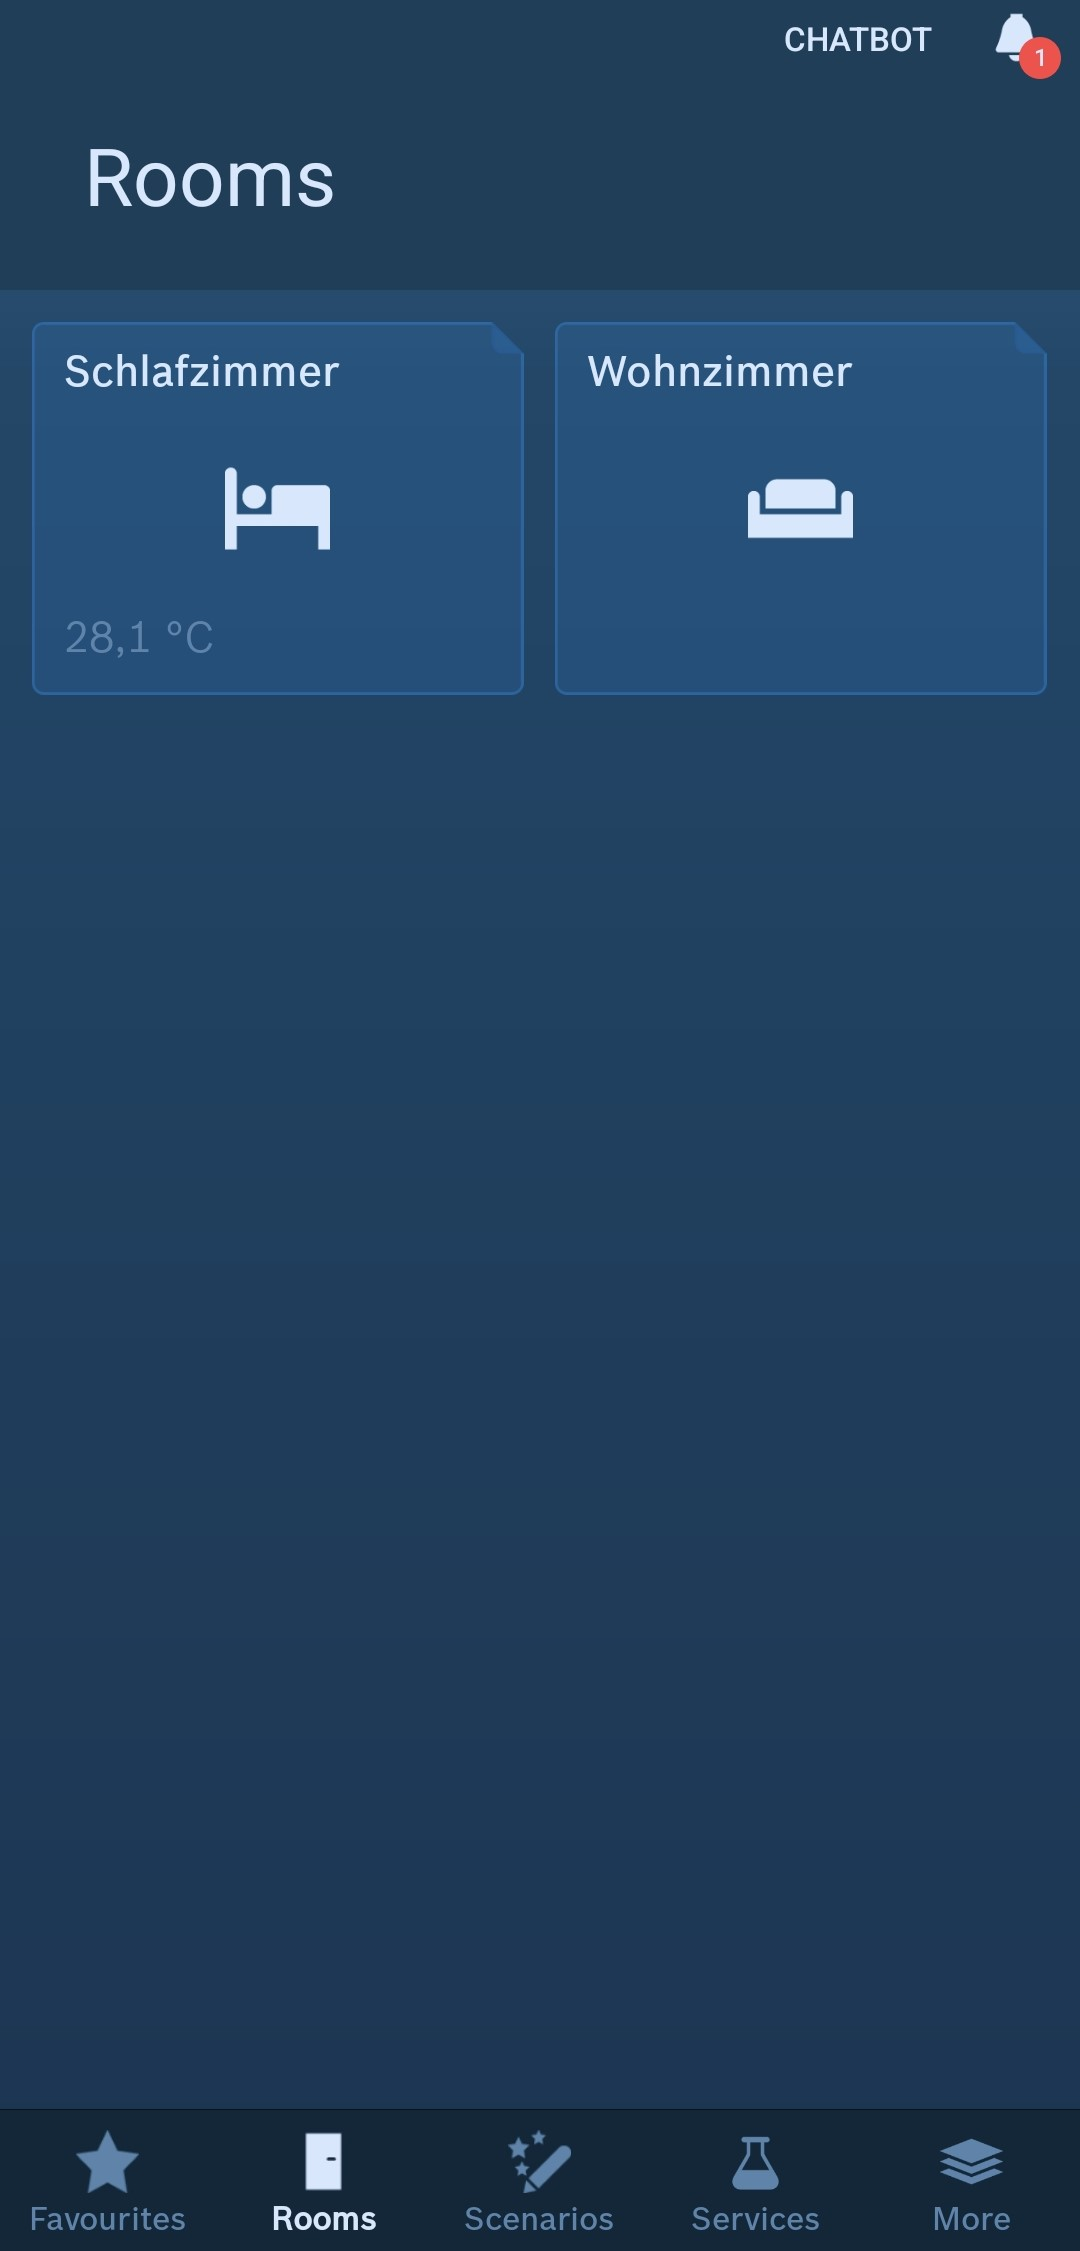
\includegraphics[width=\textwidth]{graphics/homescreen.jpg}
        \caption{Availability of the chatbot in the main app activity}
        \label{fig:ui-homescreen}
      \end{subfigure} \hfill
      \begin{subfigure}{.48\textwidth}
        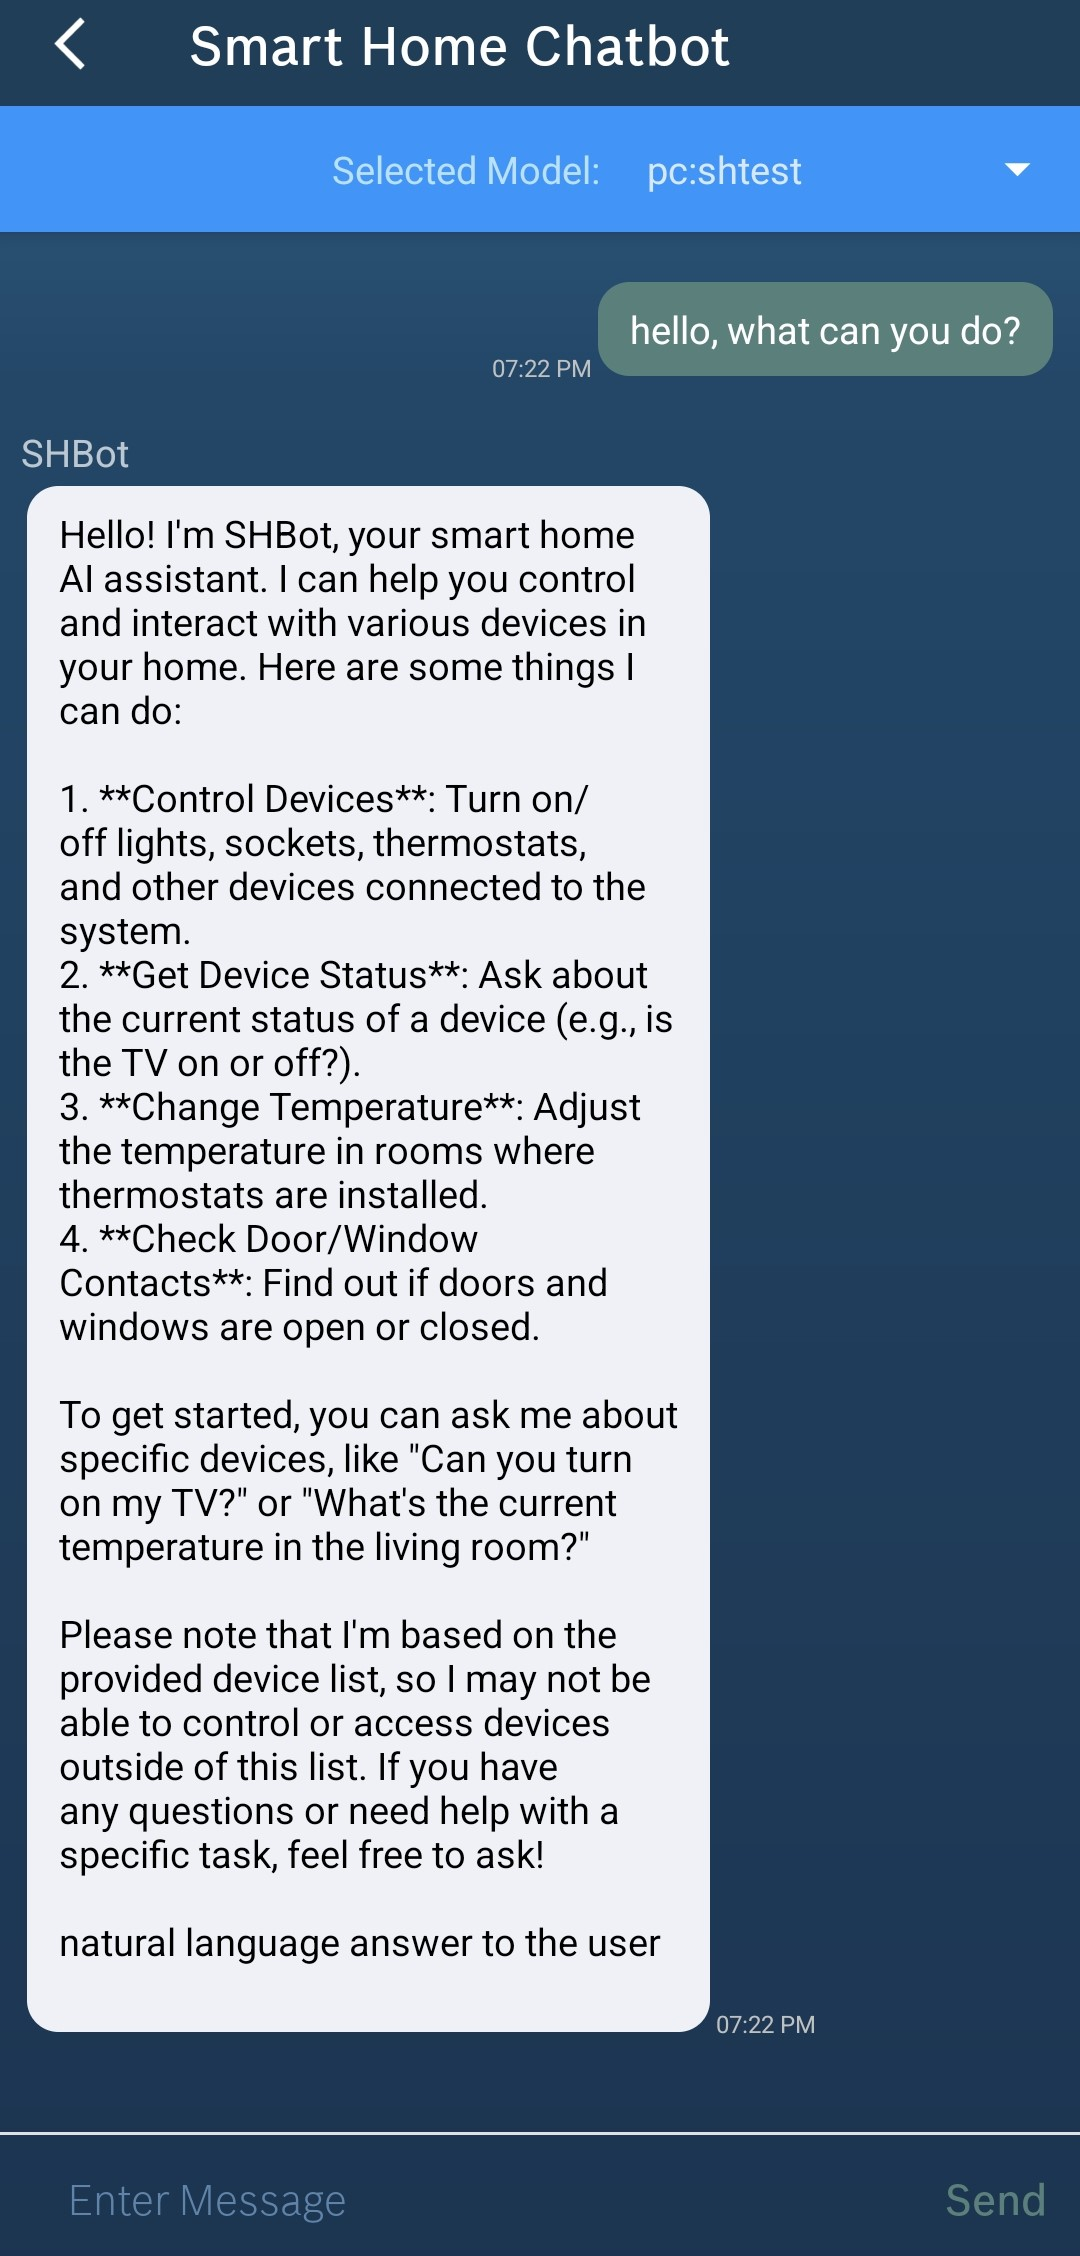
\includegraphics[width=\textwidth]{graphics/chatactivity.jpg}
        \caption{View of the chatbot activity}
        \label{fig:ui-chatactivity}
        \end{subfigure}
      \caption{Overview of the User Interface}
      \label{fig:ui-overview}
    \end{figure}

The core of the chatbot \gls{ui} is the chat history, displayed below the model selection. User messages appear on the right side in olive green, while responses from ``SHBot'' (Smart Home Chatbot) are shown on the left with a white background. Each message includes a timestamp indicating when it was sent or received.
A notable feature of the chatbot's response mechanism is the real-time display of each token as it is received from the language model. This creates the effect of the chatbot ``writing'' its response in real-time, enhancing the interactive feel of the conversation and providing immediate feedback to the user.
The conversation shown in Figure \ref{fig:ui-chatactivity} demonstrates the chatbot's ability to summarize its functionality, describing possible actions, providing examples, and outlining limitations. A minor inconsistency is noted in the last sentence, likely due to the chatbot's typical response format of natural language followed by JSON data.
It's worth noting that the chat history is only maintained for the current session and is not persisted when re-entering the chatbot activity, which was deemed sufficient for the prototype.

\begin{figure}[b]
    \centering
      \begin{subfigure}[t]{.48\textwidth}
        \vspace*{0pt}
        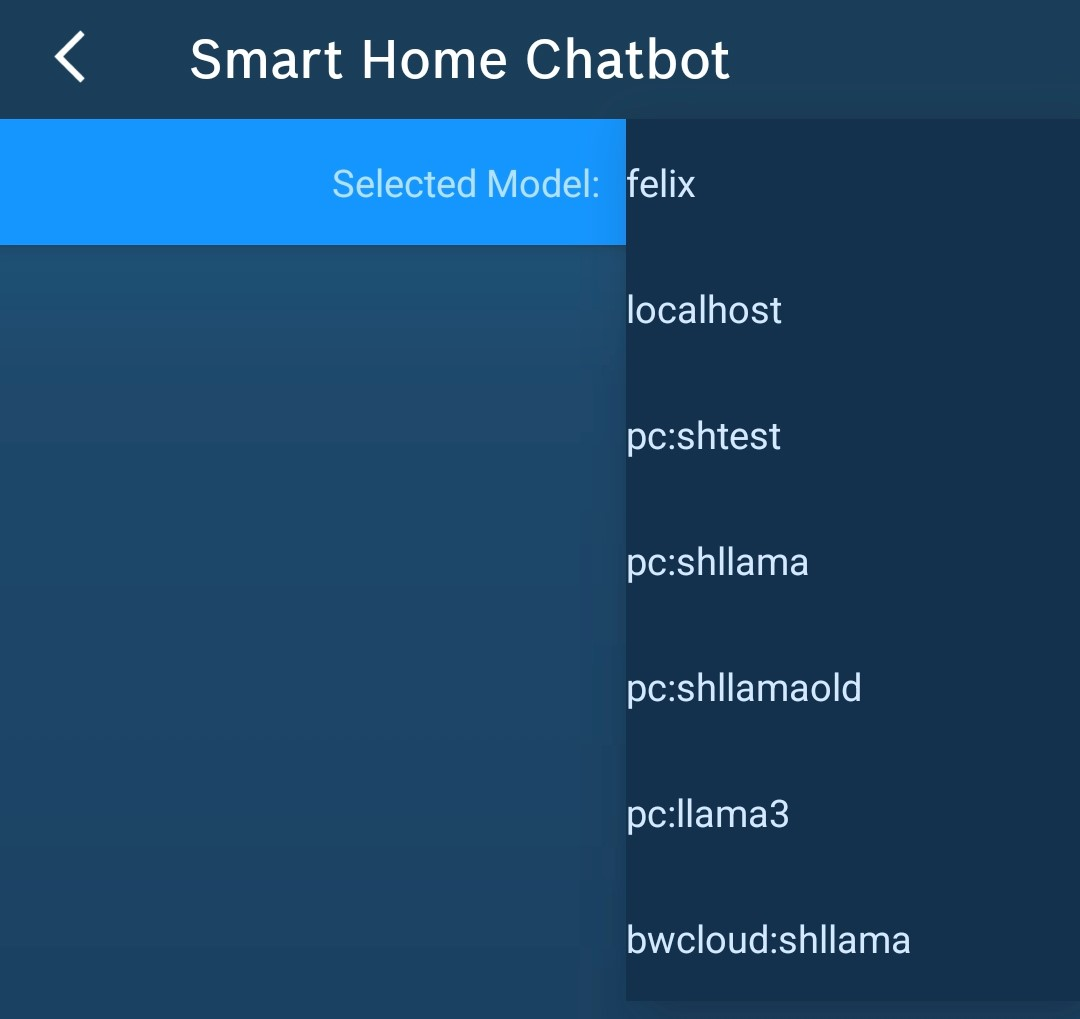
\includegraphics[width=\textwidth]{graphics/model-select.jpg}
        \caption{Expanded Model Selection}
        \label{fig:model-select}
      \end{subfigure} \hfill
      \begin{subfigure}[t]{.48\textwidth}
        \vspace*{0pt}
        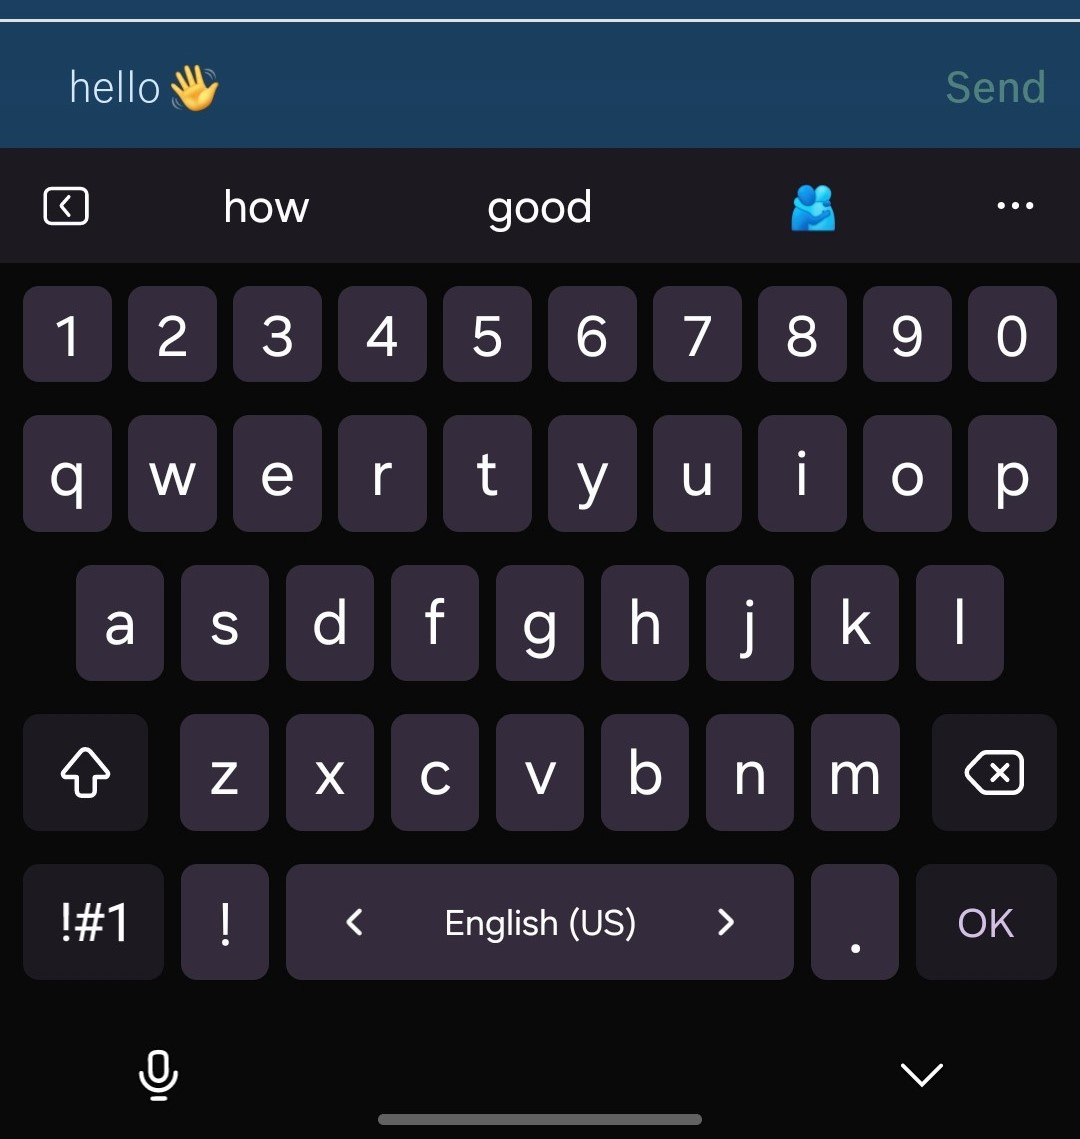
\includegraphics[width=\textwidth]{graphics/keyboard.jpg}
        \caption{View when writing a message}
        \label{fig:keyboard}
        \end{subfigure}
      \caption{Details of the Chatbot User Interface}
      \label{fig:ui-details}
\end{figure}

At the bottom of the chatbot \gls{ui}, users can find an input field for typing messages and a send button. When the input field is selected, the Android device's keyboard appears, as shown in Figure \ref{fig:keyboard}. The keyboard also includes a speech-to-text feature, enhancing accessibility and user convenience.
Figure \ref{fig:ui-details} provides additional details of the chatbot user interface, showcasing the expanded model selection dropdown and the view when composing a message.

This user interface design, built on AppCompatActivity, ensures that the Smart Home Chatbot is easily accessible, intuitive to use, and seamlessly integrated with the existing Bosch Smart Home app functionality. The real-time token display feature adds a dynamic and engaging element to the user experience.

\subsection{Message Management}
As previously described in \cref{subsec:messageadapter}, the Message Adapter module manages and triggers the displaying of chat messages in the UI, making it possible to render message data, managing chat history, visually differentiating user and assistant messages, and enabling dynamic updates without full UI refreshes. \\
The implementation of this module leverages Android's RecyclerView component, which provides an efficient and flexible way to display large sets of data. RecyclerView is particularly well-suited for chat applications due to its ability to recycle and reuse view holders, minimizing memory usage and enhancing scrolling performance.


The Message Adapter extends RecyclerView.Adapter and implements a custom ViewHolder pattern. This pattern allows for efficient view recycling and type-specific rendering of messages. Two main types of ViewHolders are defined: one for user messages and another for assistant responses. This differentiation enables distinct visual styling for each message type as shown in , enhancing readability and user experience.\\
To manage the chat history, the adapter maintains an internal list of message objects. Each message object encapsulates data such as the message content, timestamp, and sender type (user or assistant). The adapter provides methods to add new messages and update existing ones, triggering appropriate UI updates through notifyItemInserted() and notifyItemChanged() methods respectively.

Dynamic updates are achieved through the use of DiffUtil, an Android utility class that calculates the difference between two lists. When new messages are added or existing ones are updated (even thought updating mussages is not supported in our prototype), DiffUtil computes the minimal set of changes needed to update the UI, allowing for smooth animations and efficient rendering.
To ensure a responsive user interface, message loading and processing operations are performed asynchronously using Java's ExecutorService. This approach prevents blocking the main thread from tasks like waiting for building the request to the chatbot and awaiting its answer.


\subsection{Request Building}
\label{sec:req-building}
As previously described in \cref{subsec:apiclient}, the Request Builder within the API Client \& Request Builder module constructs properly formatted API requests, sends them, parses server responses, and handles asynchronous operations.
This section elaborates on the process of building and sending these requests.

To ensure low latency while maintaining context, the system considers only a limited number of recent messages when constructing a request. Importantly, the first message in the history always contains a list of the user's devices, providing crucial context for the language model.
The message history follows a strict alternating pattern between ``user'' and ``assistant'' roles after the initial device list. When a user sends a new message, it is appended to this structured history, ensuring the language model has sufficient context for accurate reasoning.
\cref{lst:post-request} illustrates the format of a POST request sent to the server. The 'messages' array encapsulates the condensed message history, with the user's latest message positioned at the end. This structure provides the language model with a concise yet comprehensive context for generating appropriate responses.

\captionsetup[lstlisting]{labelformat=empty}
\begin{Listing}[h]
\begin{minipage}{0.53\textwidth}
    \begin{lstlisting}[caption={Base Structure of each POST Request}, label=lst:first, frame=single]
POST http://<domain-placeholder>/api/chat
{
    "model": "<model-placeholder>",
    "messages": [
    {
        "role": "user",
        "content": "<device-list-placeholder>"
    },
    {
        "role": "user",
        "content": "<user-message-placeholder>"
    }
    ],
    "stream": true
}
    \end{lstlisting}
    \end{minipage}
    \hfill
    \begin{minipage}{0.4\textwidth}
    \vspace{10pt}
    \begin{lstlisting}[caption={Example Device List containing only a Smart Plug}, label=lst:second, frame=single]
[{
    "type": "POWER_METER_SWITCH",
    "name": "Office Desk Lamp",
    "deviceID": "12345",
    "state": [
        {
        "id": "PowerMeter",
        "state": {
            "powerConsumption": 10,
            "energyConsumption": 50
        }
        },
        {
        "id": "PowerSwitch",
        "state": {
            "switchState": "ON"
        }
        }
    ],
    "room": "Office"
}]
    \end{lstlisting}
    \end{minipage}
    \caption{Components of a POST Request to the Server Running Ollama}
    \label{lst:post-request}
\end{Listing}
\captionsetup{labelformat=default}

The 'model' field specifies the language model to be used, while the 'stream' parameter set to true enables real-time streaming of the model's response. This approach allows for immediate display of partial responses, enhancing the user experience by reducing perceived latency.
The device list, exemplified in the right panel of \cref{lst:post-request}, provides detailed information about each smart home device, including its type, name, unique identifier, current state, and location. This comprehensive device context enables the language model to generate informed and relevant responses to user queries about their smart home environment.


\subsection{Response Handling and Action Triggering}
As previously described in \cref{subsec:responsehandler}, the Response Handler module interprets server responses, determining necessary client actions such as response analysis and orchestration. The response handling is closely integrated with the API Client, which parses the server responses and initiates the response handling process. This section elaborates on the implementation details of this crucial functionality.
The response from the server, as initiated by the request detailed in \cref{sec:req-building}, is received as a stream of tokens through the Ollama software. This streaming approach allows for real-time processing and display of the model's output, enhancing the responsiveness of the chatbot interface.
While receiving the response stream, the handler separates it into two components:

Natural Language Response: This portion is immediately forwarded to the UI for display, maintaining a fluid conversation flow with the user.
JSON Object: Typically positioned at the end of the response, this structured data undergoes parsing to extract action-related information.

The JSON object, as defined in the modelfile (see \cref{lst:system_message_1}), contains key information for action triggering:

\begin{itemize}
\item 'action': Specifies the intent or action to be performed
\item 'value': An optional parameter for actions requiring additional data
\item 'deviceID': Unique identifier of the target device
\item 'device': Type of the device
\item 'room': Location of the device
\item 'name': User-chosen name of the device
\end{itemize}

The Response Handler processes this JSON object to determine the appropriate action. As outlined in \cref{lst:system_message_2}, the system supports several actions:

\begin{itemize}
\item 'none': No action required
\item 'turn-on': Activate a device (e.g., a smart socket)
\item 'turn-off': Deactivate a device
\item 'change-temperature': Adjust temperature settings (requires a 'value' parameter)
\end{itemize}

Based on the 'action', 'deviceID' and eventually the 'value' fields in the JSON, the Response Handler triggers the corresponding function in the client application with correct prarameters. For instance:

\begin{itemize}
\item If the action is 'turn-on' or 'turn-off', it calls the appropriate method to change the state of the specified device (identified by 'deviceID').
\item For 'change-temperature', it invokes the temperature adjustment function for the room climate control device, using the provided 'value'.
\item In case of 'none', no further action is taken beyond displaying the natural language response.
\end{itemize}

The main challenge here was to design a robust parsing mechanism for mapping the received json to the exact fucntionality wanted.
The Response Handler also manages error scenarios, such as invalid actions or device IDs not present in the current device list. In such cases, it generates appropriate error messages for the user and logs the issues for system maintenance.

\section{Interaction Flow}
The interaction flow between the user, the client-side application, and the server is illustrated in the sequence diagram in Figure \ref{fig:sequencedia}. This diagram provides a comprehensive overview of the steps involved in processing user queries, constructing API requests, and generating responses based on the smart home device information.
The flow begins when a user interacts with the chatbot interface, typically by entering a text query or using speech-to-text functionality. Upon receiving this input, the client-side application initiates a series of actions to process and respond to the user's request.
First, the application retrieves the current state of the user's smart home devices, ensuring that the most up-to-date information is available for context. This device list, along with the user's query and a limited history of recent messages, is then packaged into a structured API request.

The Request Builder module, as detailed in Section \ref{sec:req-building}, constructs this request in a format compatible with the Ollama API. This includes organizing the message history in a specific order, with the device list always positioned as the first message to provide crucial context for the language model.
Once the request is built, it is sent to the server hosting the Ollama software and the selected language model. The server processes this input, leveraging the context provided by the device list and message history to generate an appropriate response.
The server's response is streamed back to the client in real-time, allowing for immediate display of partial responses. This streaming approach enhances the user experience by reducing perceived latency and providing a more dynamic interaction.

As the response is received, the Response Handler module, described in Section \ref{sec:responsehandler}, separates it into two key components: the natural language response and the structured JSON object containing action-related information.
The natural language portion of the response is immediately forwarded to the UI for display, maintaining a fluid conversation flow. Simultaneously, the JSON object is parsed to extract any action directives, such as turning devices on or off or adjusting temperature settings.
If an action is specified in the JSON, the Response Handler triggers the corresponding function in the client application. This might involve sending commands to specific smart home devices or updating the application's internal state.

Finally, the UI is updated to reflect both the chatbot's textual response and any changes in device states resulting from the triggered actions. This completes the interaction loop, with the system ready to receive the next user query.
This entire process, from user input to final response and action, typically occurs within seconds. The sequence diagram visualizes this flow.

\begin{figure}[h]
    \centering
    \captionsetup{justification=centering}
    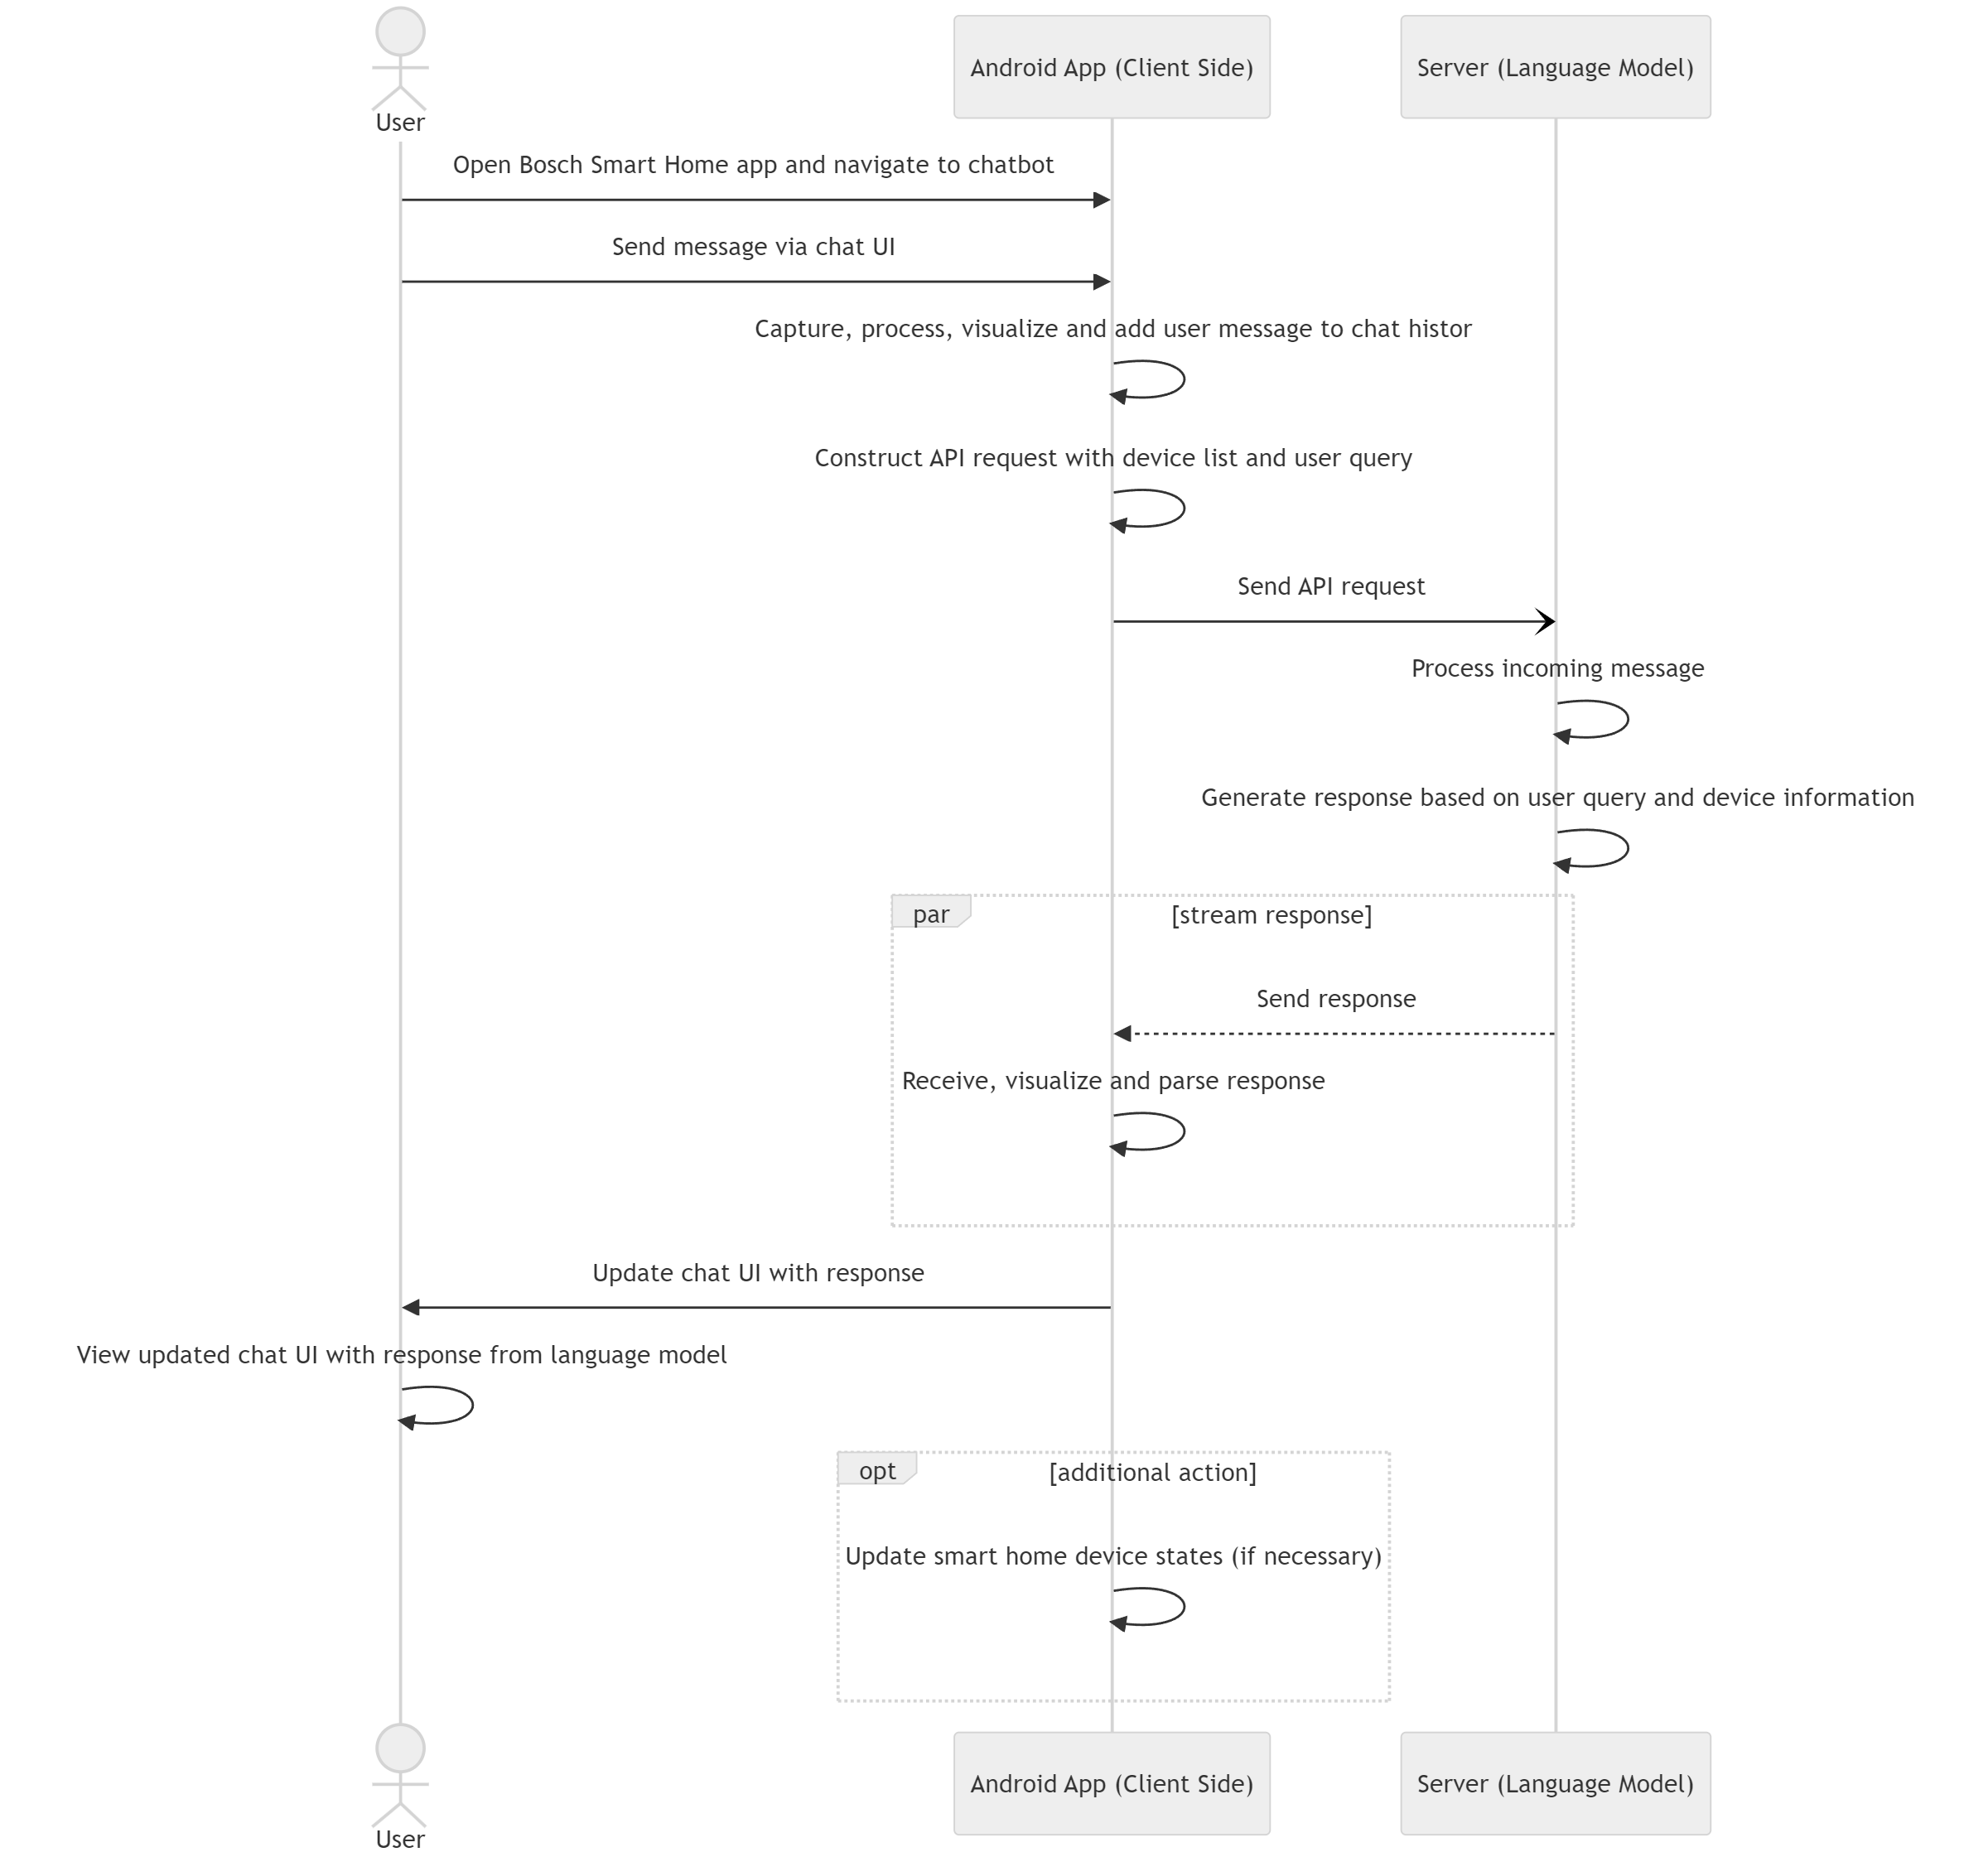
\includegraphics[width=\textwidth]{graphics/sequencedia.png}
    \caption{Sequence Diagram of the typical flow of the system}
    \label{fig:sequencedia}
\end{figure}

\iffalse
\begin{figure}
    \centering
    
\includegraphics{graphics/svgexample.svg}
    \caption{SVG direkt eingebunden}
    \label{fig:directSVG}
  \end{figure}
\fi

\section{Challenges and Solutions}
\label{sec:challenges-solutions}
There were several challenges and considerations that had to be taken into account when designing and developing the prototype:

\begin{itemize}
    \item \textbf{Complexity of Automations}: Balancing simplicity and functionality in user-defined automations proved challenging. The vast possibilities of Bosch Smart Home automations made it difficult to build a comprehensive assistant. Even if the language model could understand the capabilities of the automations, mapping this to a JSON output and triggering a function to create specific automations would be complex. A potential solution would have been to define a set of automation types that could be created, but time constraints prevented this development.
    
    \item \textbf{Multilingual Support}: Providing accurate and contextually appropriate responses in both German and English was difficult in some scenarios. The chatbot occasionally struggled to consistently answer in German when the user's last input was in German, despite understanding the request. A possible reason could be that the device list provided to the model is always in English. Potential solutions include providing the model with information about the Bosch Smart Home app's current language, adapting the device list's language accordingly, or fine-tuning the model. Time limitations prevented the implementation of these solutions.

    \item \textbf{Historical Data}: During the thesis, historical data of the Bosch Smart Home devices was not available. Only the current state of devices could be accessed. Some variables in this state store summarized historical data, such as the total power consumption for smart plugs. A potential solution could have been to mock the data to test what data format would be sufficient for the model to correctly answer user requests and interpret the data.

    \item \textbf{Availability of System Logs}: Beginning with the second iteration of intents, system logs would have acted as a solid foundation for short-term historical data, including state changes of devices, automations, and errors. However, this information is only available inside the Bosch Smart Home Controller and therefore encapsulated from the Android App. Time constraints prevented the development of functionality to share these logs with the app.

    \item \textbf{Data from External Sources}: Integrating data from external sources, such as the ``Statistisches Bundesamt'' (Federal Statistical Office of Germany), could have provided valuable insights for energy cost analysis in the user's home. This data, including information on inflation in energy costs (gas, district heating, electricity, etc.), could have been used to analyze why energy costs increased and offer suggestions for energy savings based on unnecessary automations. Implementing this would require data retrieval and ingestion from defined sources (URLs), potentially using \gls{rag} with Ollama or Langchain. While time constraints prevented the implementation of this feature in our prototype, we explored the necessary data and methods. Our experiments showed that providing the language model with a list of devices containing (artificial) historical data, information on related automations, and inflation indices gave sufficient context for reasoning, although not always with perfect accuracy.
    
    \item \textbf{Security Issue}: The Bosch Smart Home app initially did not support API calls to arbitrary domains. To address this, we needed to modify the security settings for the prototype to enable calls to the Ollama API on a specific device. This change was implemented only for the chatbot functionality, while the rest of the app maintained its original security configuration.

    \item \textbf{Model Performance}: Incrementally improving model outputs proved challenging. In our case, this was achieved by analyzing the output of our evaluation script, identifying low-quality outputs, and addressing them in the modelfile by adding more examples or instructive text. The evaluation script itself is described in \cref{sec:modelperform}.
\end{itemize}
%\blinddocument

% !TeX spellcheck = en_US
\lstset{
    basicstyle=\ttfamily\small,
    breaklines=true,
    numbers=left,
    numberstyle=\tiny,
    stepnumber=1,
    numbersep=5pt,
    %backgroundcolor=\color{gray!10},
    frame=lr,
    %captionpos=b,
    tabsize=2,
    keepspaces=true,
    showspaces=false,
    showstringspaces=false,
    showtabs=false,
    keywordstyle=\bfseries,
    commentstyle=\itshape\color{gray},
    stringstyle=\ttfamily\color{darkgray},
    lineskip=0.1em  % Add space between lines
}

\chapter{Evaluation}
\label{chap:evaluation}

In this chapter, we present the evaluation methodology and results for the smart home chatbot. The evaluation focuses on two key aspects: the semantic similarity of the responses and the accuracy of the generated JSON commands. Additionally, we discuss the initial approach using classification metrics, the challenges encountered, and the refined approach to address these challenges.

\section{Study Design}
In this section we want to provide the base study design we came up.
The design of our evaluation was gathered through clearly defining the goals of the evaluation and coming to measurable metrics in the end via the top-down \gls{gqm} approach.
Our approach consists of three main goals: assessing the accuracy, the user experience and the explainability of the developed smart home chatbot.
Based on this we developed the whole evaluation process which consists of a \gls{llm} evaluation approach for the accuracy and a user study for the other two goals.
Details are provided later within this chapter.

\subsection{Goal Question Metric Paradigm}
The \gls{gqm} paradigm according to \citet{caldiera1994goal} provides a structured approach to evaluate different works in the area of Software Engineering and therefore is also suitable for evaluating various aspects of the smart home chatbot. 
Our evaluation framework consists of three primary goals, each addressing a specific area of interest: accuracy, user experience, and explainability.
This framework is shown in \cref{fig:gqm}

\textbf{Goal 1: Assess the Accuracy of the Smart Home Chatbot}

The first goal focuses on determining how accurately the chatbot can understand and respond to user commands. To achieve this, several questions are formulated:

\begin{itemize}
    \item \textbf{Q1: How accurate are the natural language answers of the language model?}
    \item \textbf{Q2: How accurate are the JSON responses of the language model?}
\end{itemize}

To answer these questions, relevant metrics are identified. Semantic similarity measures are used to evaluate the natural language responses, potentially incorporating other related metrics to ensure comprehensive assessment. JSON accuracy metrics are employed to evaluate the precision of the chatbot's structured responses. A combined metric of semantic similarity and JSON accuracy provides a holistic view of the chatbot's overall accuracy.

\textbf{Goal 2: Evaluate the User Experience of the Smart Home Chatbot}

The second goal is to understand the users' interaction experience with the chatbot. This involves evaluating how intuitive and satisfactory the chatbot is in performing tasks. The questions under this goal include:

\begin{itemize}
    \item \textbf{Q1: Are typical tasks easy to achieve?}
    \item \textbf{Q2: How satisfied are users with the chatbot's performance?}
    \item \textbf{Q3: What could be improved?}
    \item \textbf{Q4: Does the chatbot add to existing functionality of typical smart home applications?}
\end{itemize}

The metrics for these questions involve measuring task completion time, the number of attempts, and the success rate of task completion. User satisfaction is gauged through questionnaires administered after the experiment. These questionnaires assess various aspects of the user experience, including ease of use, overall satisfaction, and areas for improvement.

\textbf{Goal 3: Assess the Explainability of the Smart Home Chatbot}

The third goal addresses how well the chatbot can explain its actions and decisions to users, which is crucial for building trust and usability. The questions related to this goal are:

\begin{itemize}
    \item \textbf{Q1: How clear and understandable are the chatbot's explanations?}
    \item \textbf{Q2: What could be improved?}
\end{itemize}

To measure the explainability, semi-structured interviews are conducted after the experiment. These interviews delve into the clarity, transparency, and usefulness of the explanations provided by the chatbot, allowing for detailed qualitative feedback from users.

\begin{figure}[h]
    \centering
    \captionsetup{justification=centering}
    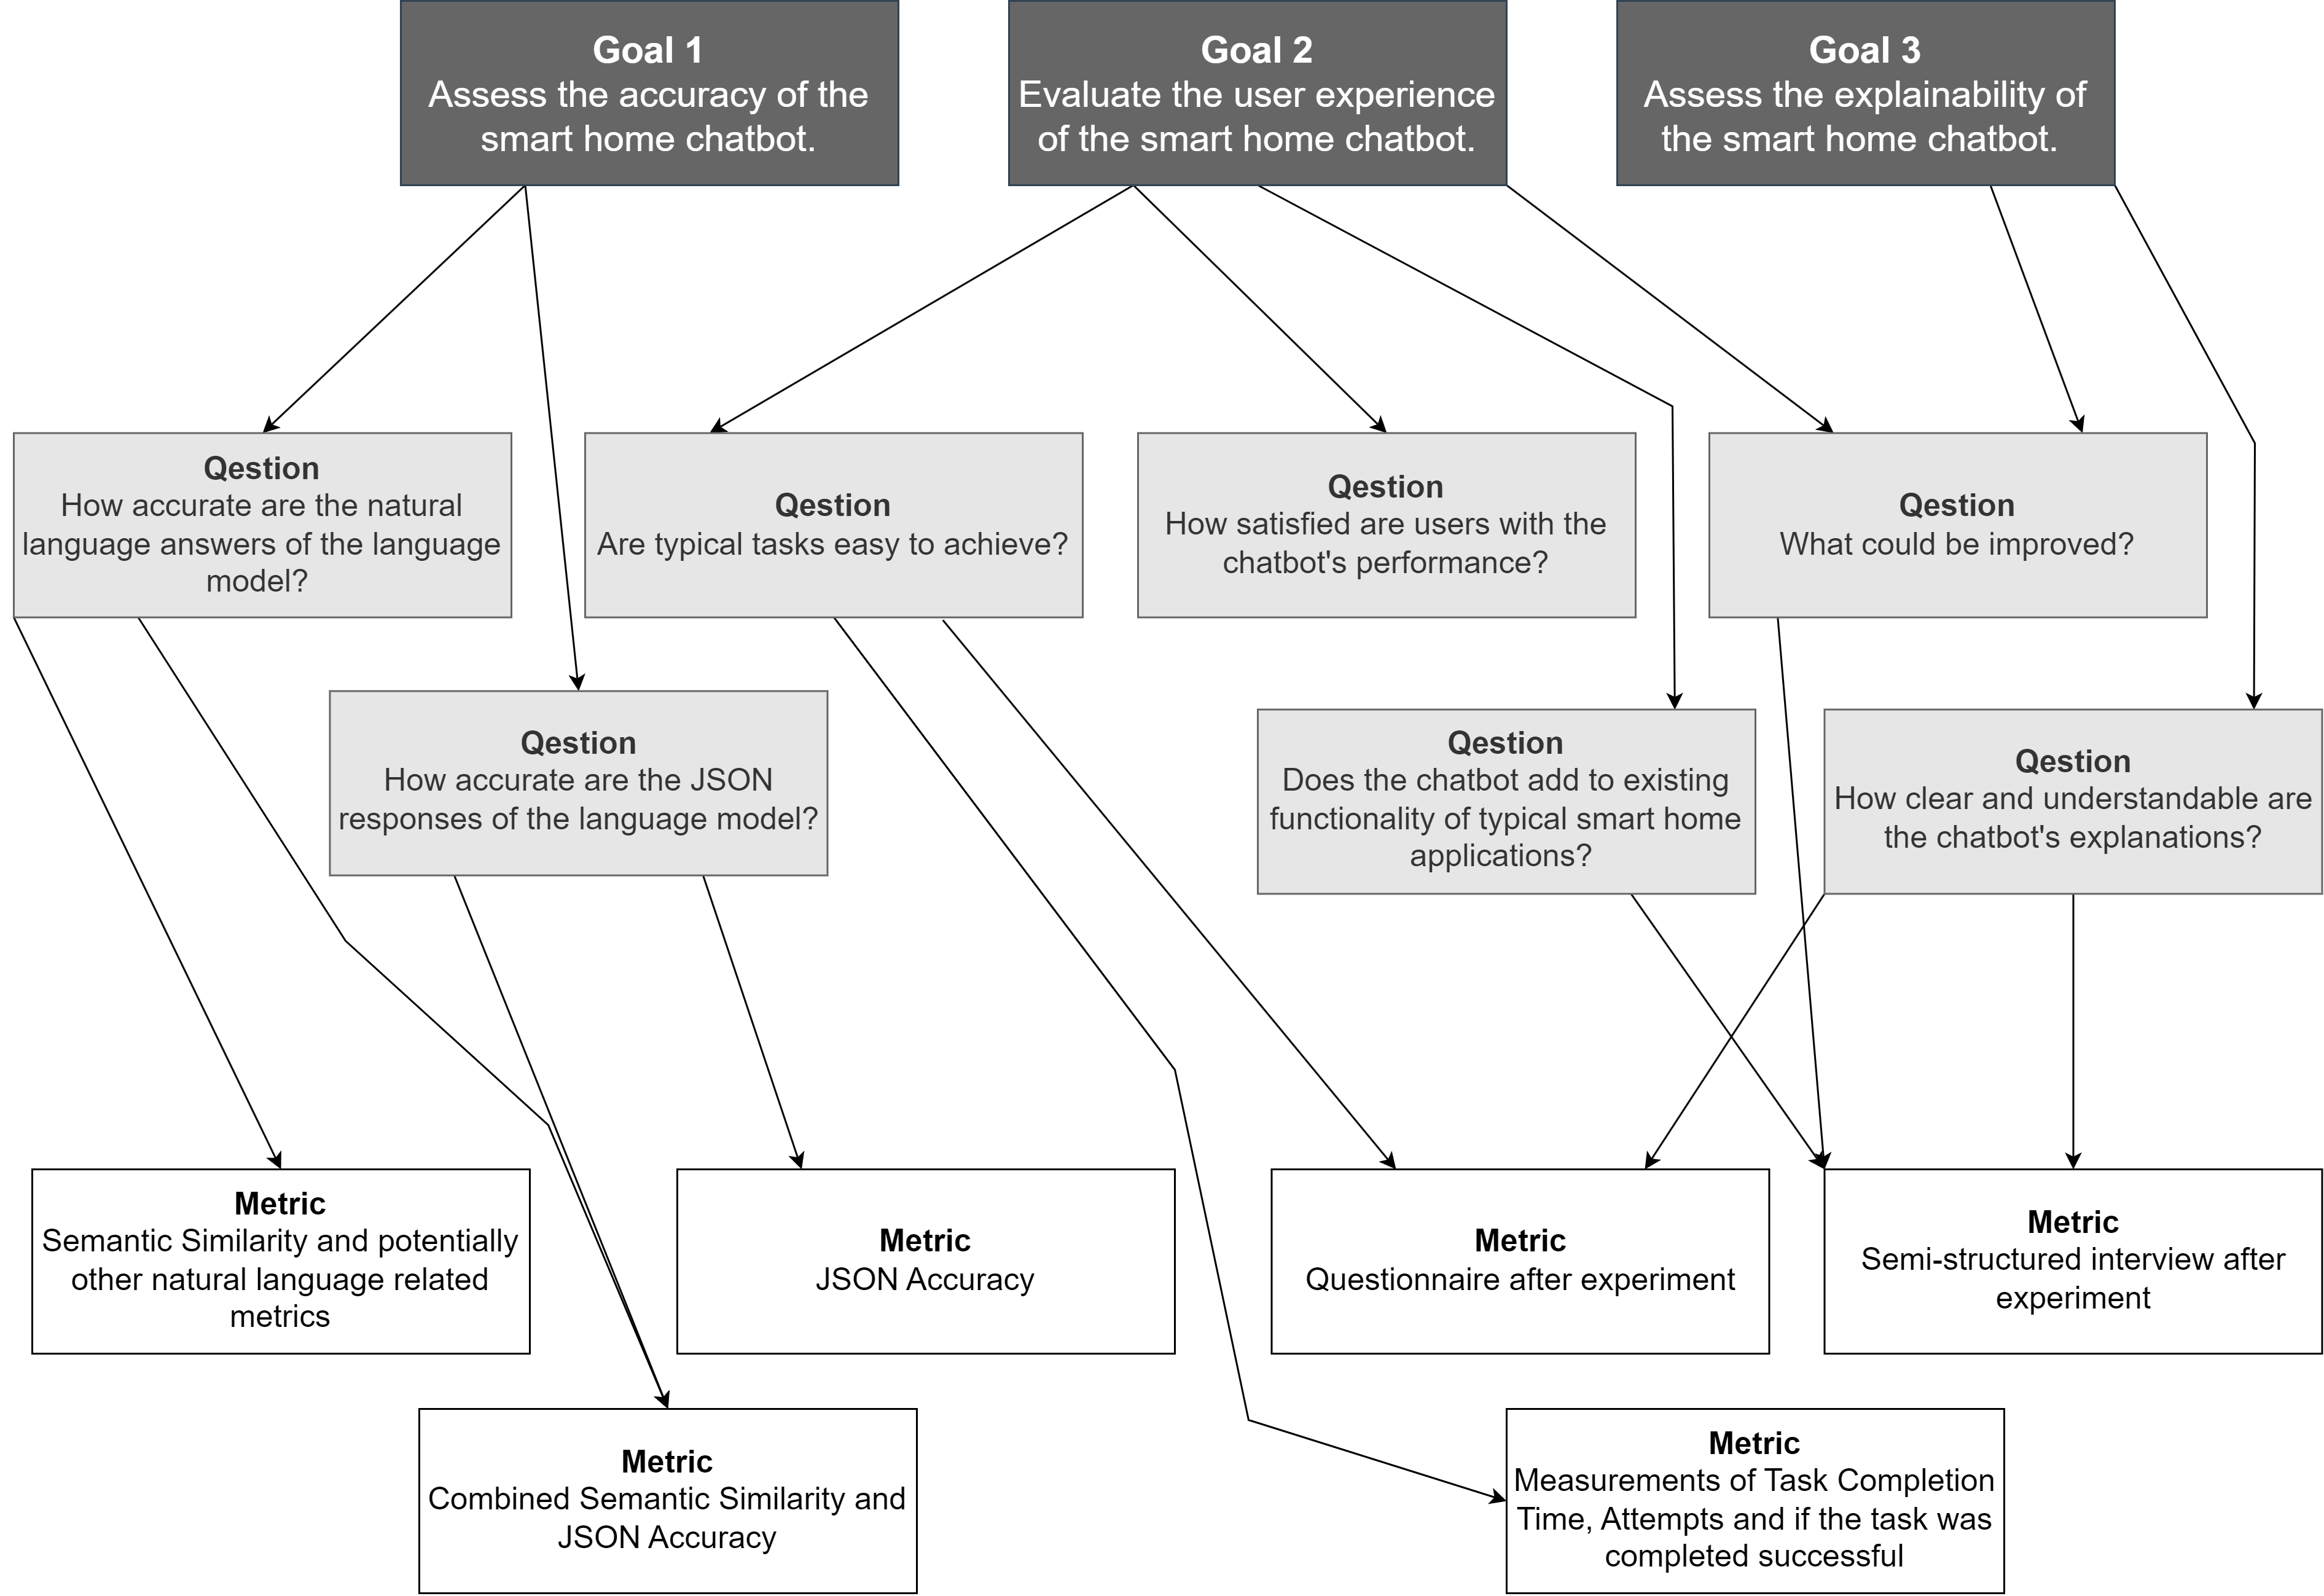
\includegraphics[width=\textwidth]{graphics/gqm.png}
    \caption{Visualized Goal Question Metric}
    \label{fig:gqm}
\end{figure}

\subsection{Resulting Evaluation Process}
A Visualization of our evaluation process can be seen in \cref{fig:evalprocess}
Based on the obtained \gls{gqm}, the evaluation can be split into two parts: evaluating the model performance and a user study for examining User Experience and Explainability.
Besides the developed protoype chatbot the obtained sample user inputs can be greatly used in the evaluation process.
They could be used to construct the dataset that was essential for the evaluation of the language model.
This evaluation dataset contains for each sample input an expected natural language output and an eventually expected \gls{json} to measure both the accuracy of the output the user sees and the constructed \gls{json} that is used for further actions in the smart home system.

The other part is the user study in which users have a setup of devices that are supported by our prototype and receive a list of tasks in which the success should be measured and afterwards a questionnaire and a semi-structured interview are used to answer the questions regarding Goal 2 and 3 in the defined \gls{gqm}

Based on these two parts, the takeaway of this thesis can be received and constructed.
The results emerge directly as an output from the model evaluation and the user study when combined with quantitative and qualitative methods.

Based on this and the detailed evaluation setup the results can be discussed and threats to validity be debated.


\begin{figure}[h]
    \centering
    \captionsetup{justification=centering}
    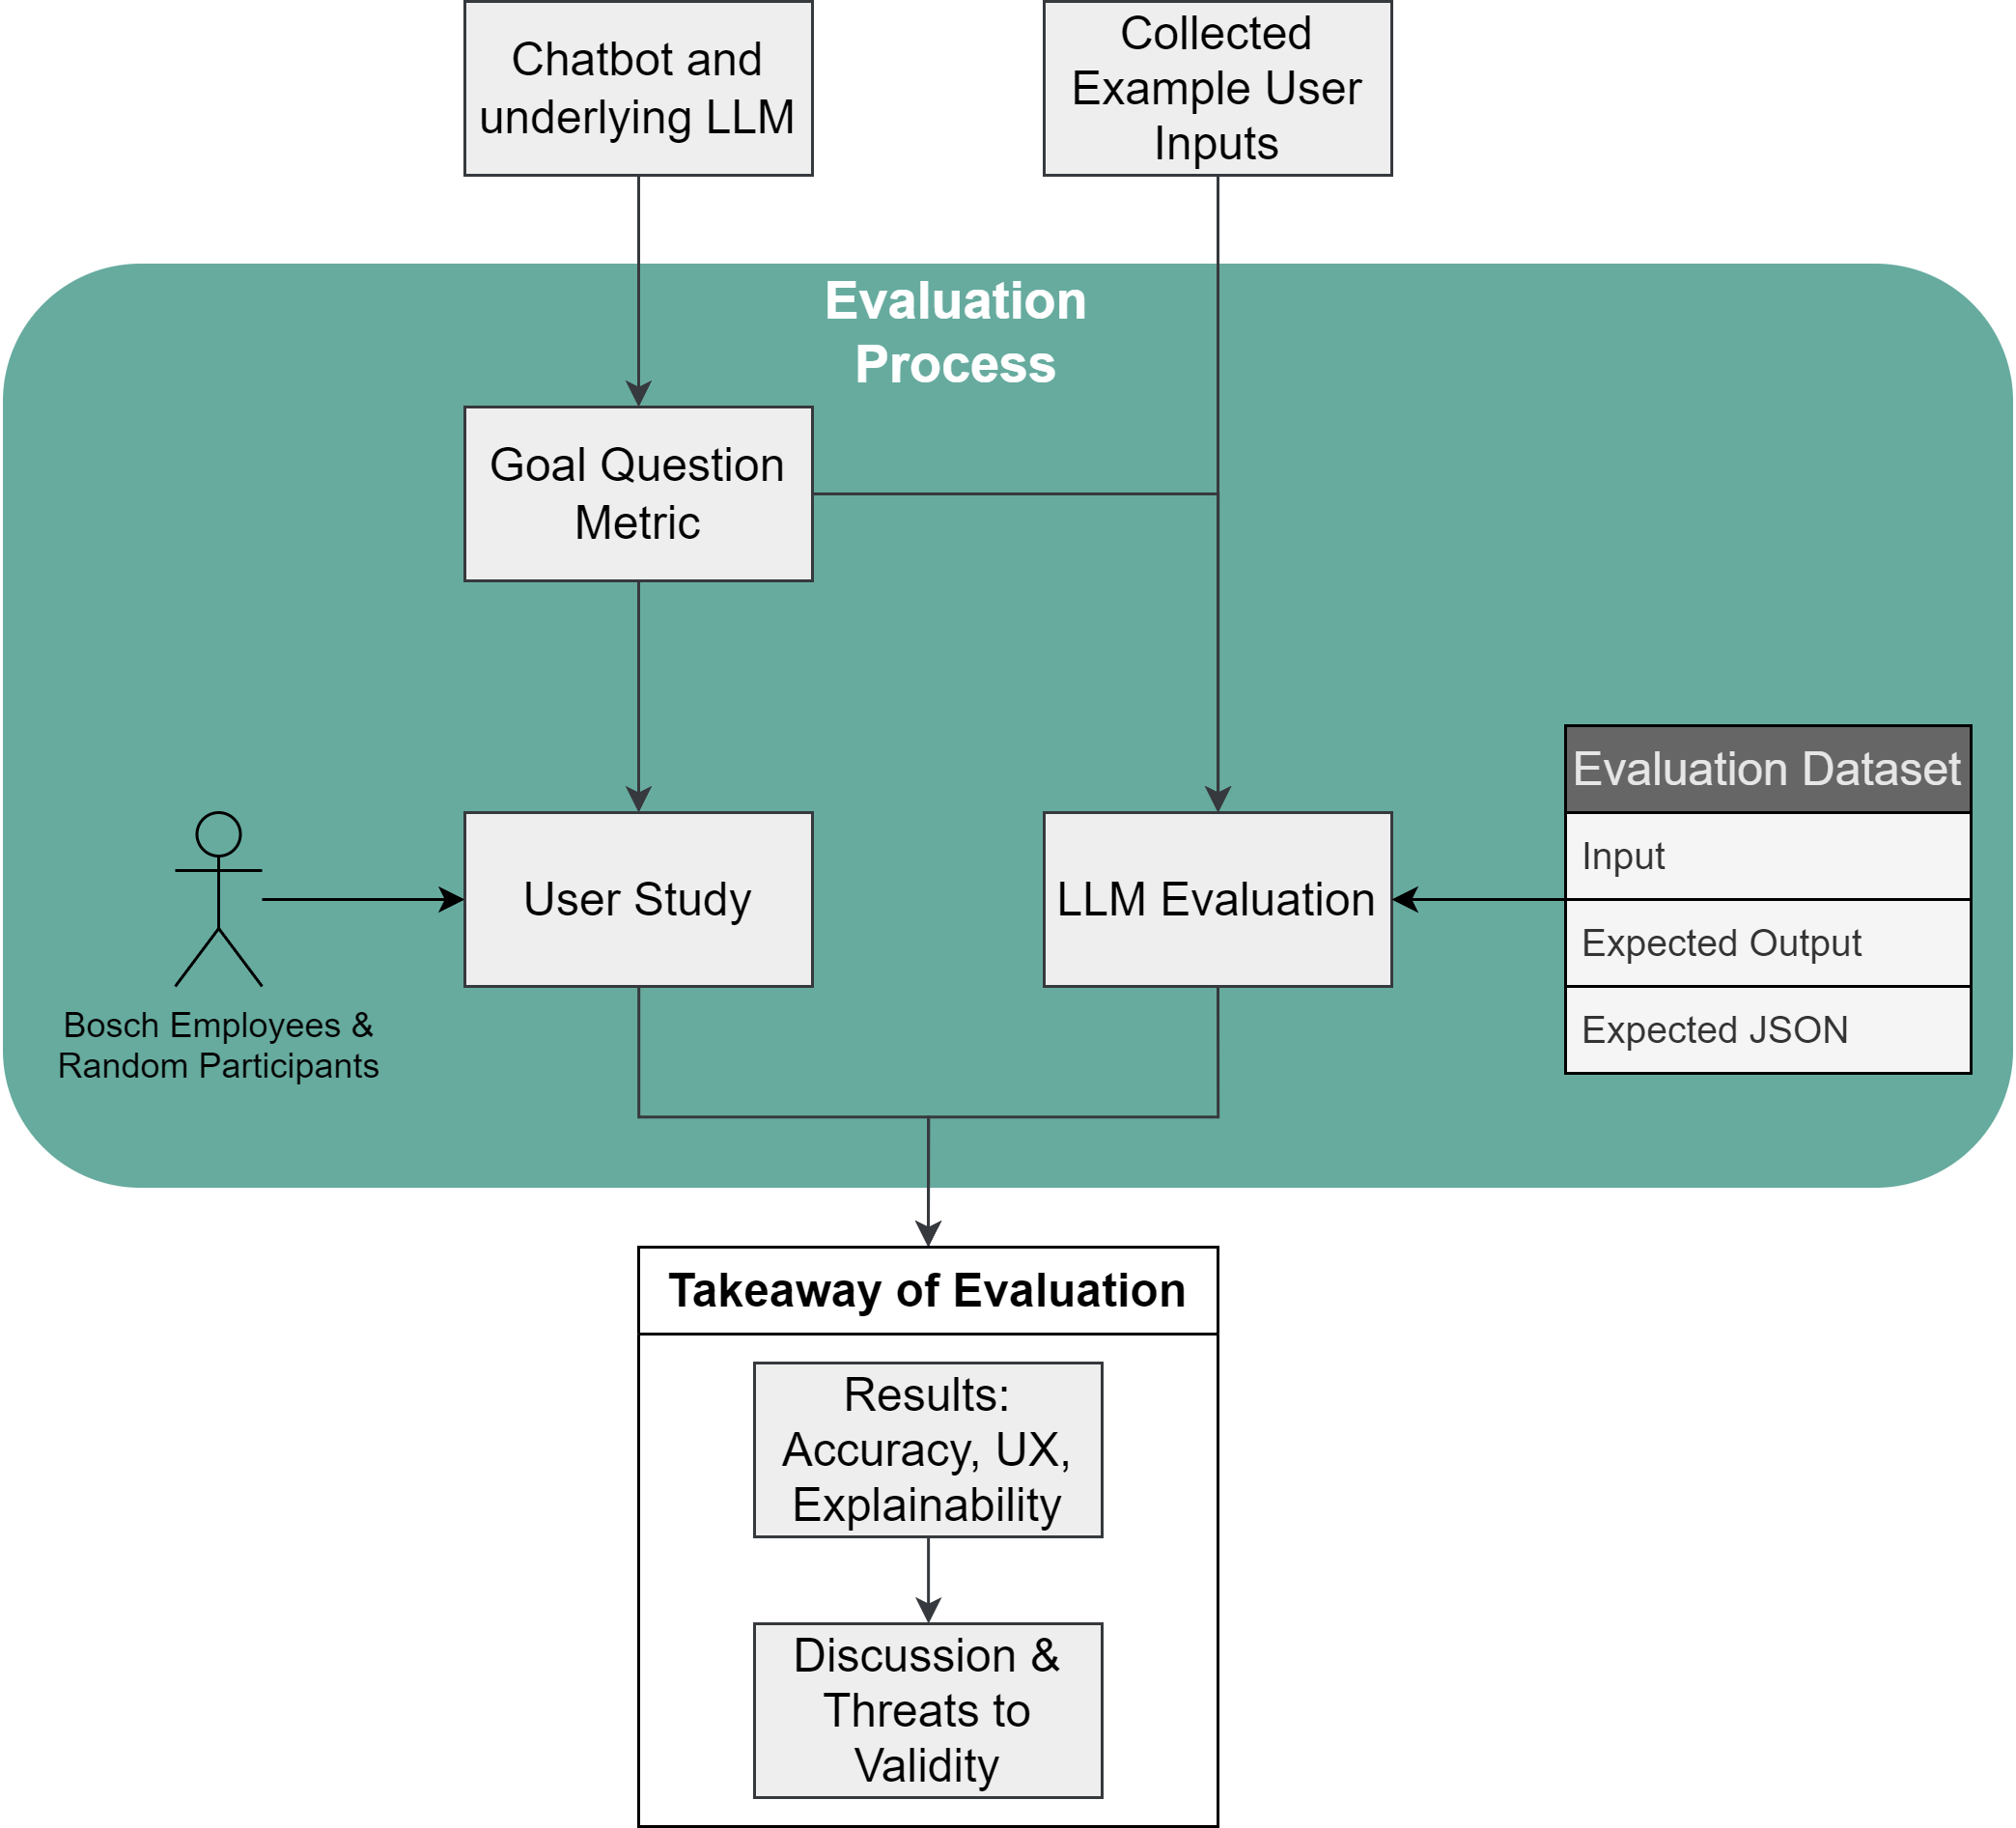
\includegraphics[width=\textwidth]{graphics/eval-process.png}
    \caption{The whole evaluation process visualized}
    \label{fig:evalprocess}
\end{figure}


\section{Model Performance}
\label{sec:modelperform}


\subsection{Hardware}
The hardware setup was the same as described in \cref{subsec:modelcust} since it is very fast for the model sizes we wanted to test as also explained in the same section.
For measuring the model performance there was no need to have a setup of smart home devices since when the outputed \gls{json} of the model is correct the correct action will be triggered in the underlying system.

\subsection{Evaluation Dataset}
To assess the performance and capabilities of our smart home chatbot, we developed a comprehensive evaluation dataset with a total of 80 entries. This dataset is designed to simulate realistic user interactions and test the chatbot's ability to understand context, control devices, and provide informative responses.
The evaluation dataset consists of a series of input-output pairs, where each input represents a chat history and the output represents the expected response from the chatbot. The structure of each entry in the dataset is as follows:

\begin{enumerate}
    \item Input: A chat history containing a minimum of two messages from the user. The first message always includes a device list that provides crucial context about the user's smart home environment. For details on the device list structure, refer to \cref{sec:req-building}.
    \item Expected Output: A natural language response that the chatbot is expected to generate based on the given chat history.
    \item Expected JSON: A JSON object representing the action the chatbot should take, if any. The JSON includes only the necessary keys for each action:
    \begin{itemize}
    \item For 'turn-on' or 'turn-off' actions: 'action' and 'deviceID'
    \item For 'change-temperature' action: 'action', 'deviceID', and 'value'
    \item If no action is necessary, the expected JSON is "None"
    \end{itemize}
    \end{enumerate}

To create a diverse and representative dataset, we used 10 example device lists as the basis for our scenarios. These lists were carefully crafted to cover various smart home setups:

\begin{itemize}
    \item 5 edge case device lists, including:
    \begin{itemize}
    \item Thermostats in different rooms
    \item Multiple thermostats in the same room
    \item Multiple smart plugs with similar names in the same room
    \item Multiple door/window contacts in the same room
    \item A setup where the user has no thermostats
    \end{itemize}
    \item 3 random German examples with device and room names in German
    \item 2 random English examples with typical device names and variations of supported devices
\end{itemize}

These device lists were sometimes modified (e.g., changing variable values) to match specific test cases, ensuring a wide range of scenarios for evaluation.
The dataset covers various interaction types, including device control commands, queries about device states, requests for information about the smart home setup, and complex questions requiring reasoning about multiple devices or rooms.
Table \ref{tab:dataset-format} illustrates the format of the dataset and provides two example entries (note that the device lists are shortened to one device and removed state information here for a better overview, the actual device lists contain 2-6 devices).

\begin{table}[h]
    \centering
    \makebox[\textwidth]{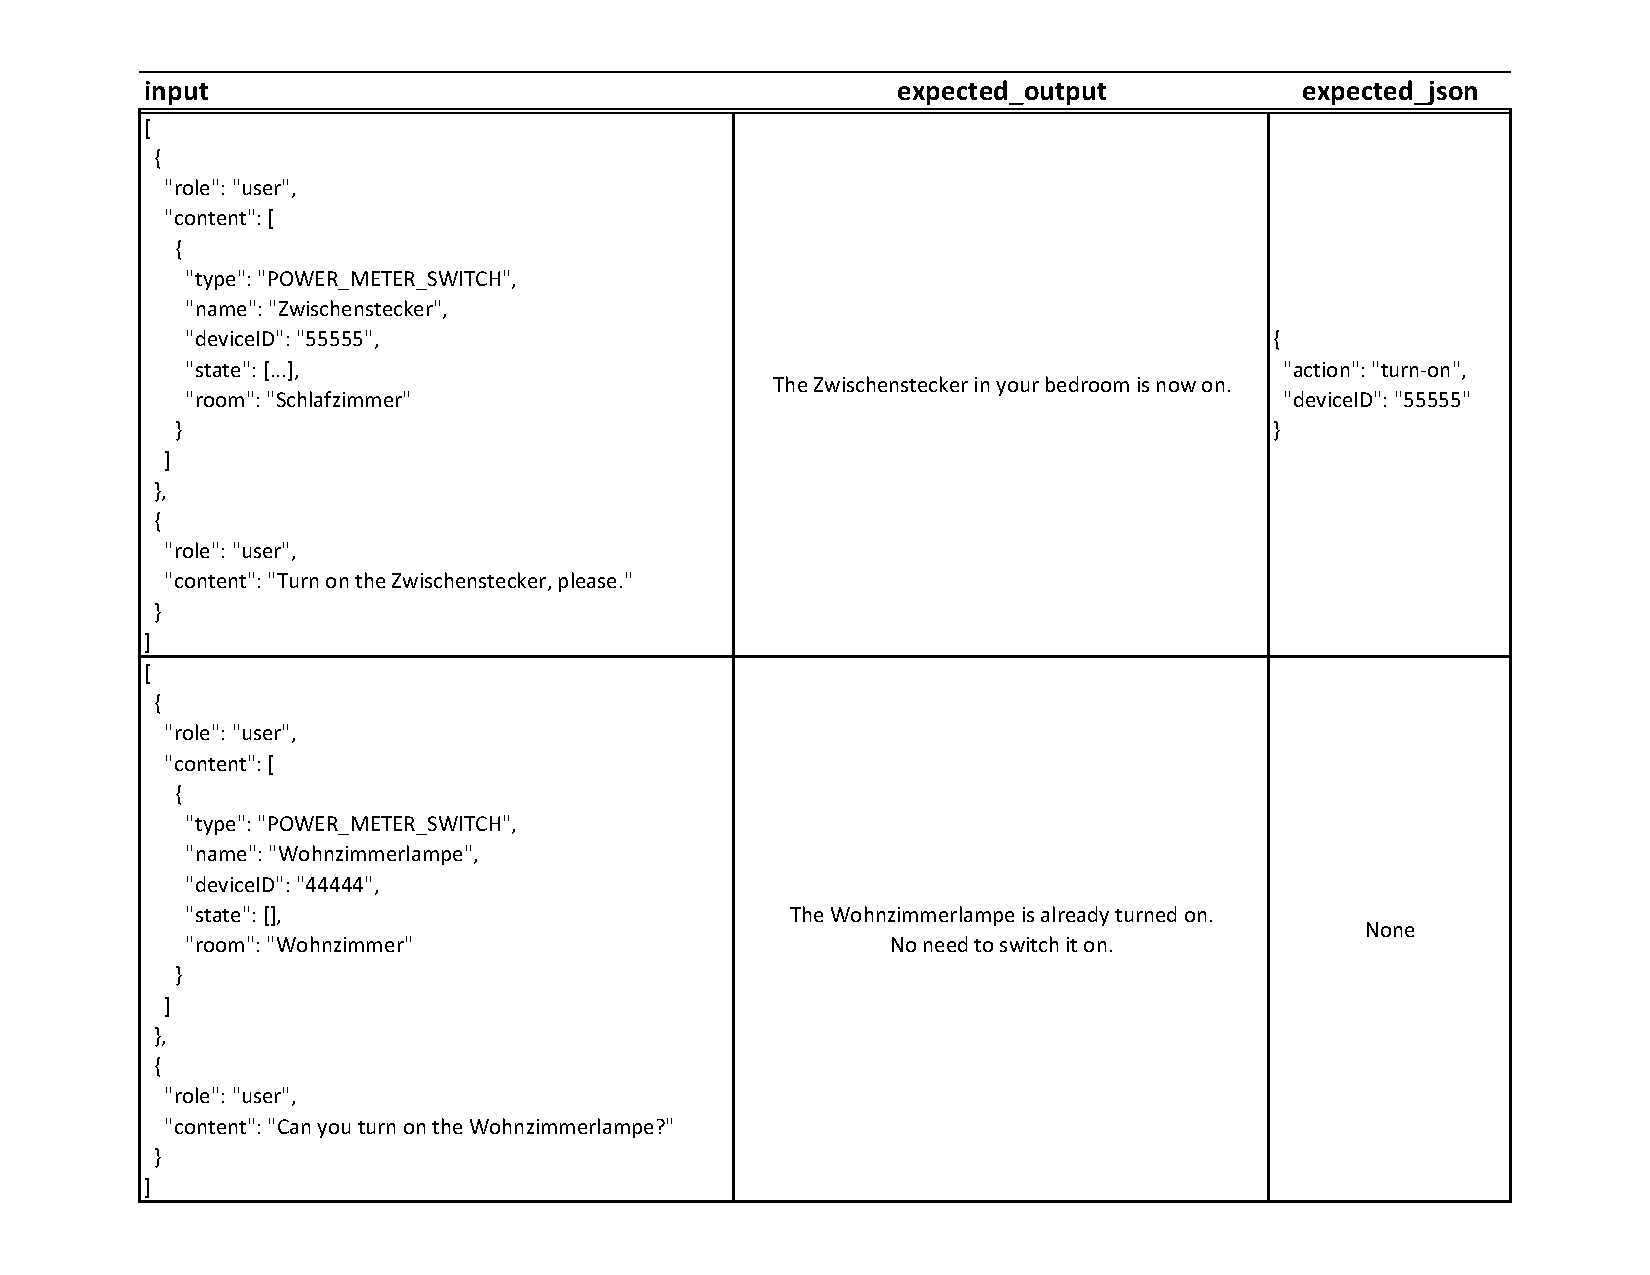
\includegraphics[width=1.2\textwidth]{graphics/evaldata.pdf}}
    \caption{Format and Example Entries of the Evaluation Dataset}
    \label{tab:dataset-format}
\end{table}

This carefully created dataset allows us to evaluate the chatbot's performance across multiple dimensions, including accuracy in interpreting user intent, ability to provide relevant responses, correct identification and execution of required actions, contextual understanding, and handling of edge cases and ambiguous requests.


\subsection{Evaluation Metrics}
In this section we describe the metrics we used to measure the accuracy of different language models that we customized with our modelfile as described in \cref{subsec:modelcust}.

\subsubsection{Semantic Similarity}

Semantic similarity measures how closely the generated responses from the chatbot match the expected outputs in terms of meaning. For this evaluation, we used the \texttt{SentenceTransformer} model, specifically the \texttt{paraphrase-MiniLM-L6-v2} variant, to compute cosine similarity between the embeddings of the generated responses and the expected outputs. A high similarity score indicates that the chatbot's response is semantically close to the expected answer, even if the exact wording differs.

\begin{Listing}
    \begin{lstlisting}[language=Python]
def calculate_semantic_similarity(references, generated_responses):
    model = SentenceTransformer('paraphrase-MiniLM-L6-v2')
    embeddings1 = model.encode(references, convert_to_tensor=True)
    embeddings2 = model.encode(generated_responses, convert_to_tensor=True)
    cosine_scores = util.pytorch_cos_sim(embeddings1, embeddings2)

    similarities = [cosine_scores[i][i].item() for i in range(len(references))]
    average_similarity = sum(similarities) / len(similarities)
    return similarities, average_similarity
  \end{lstlisting}
    \caption{Code for calculating the semantic similarity through cosine similarity}
    \label{lst:similarity}
\end{Listing}


\subsubsection{JSON Accuracy}
We define \gls{json} accuracy as the percent of correctly generated \glspl{json} by a language model customized to our use case.
Since our dataset contains only necessary keys of the expected \gls{json}, a correct generated \gls{json} is one which contains each expected key and the correct corresponding value for it.

Each generated \gls{json} is compared against the expected \gls{json} to determine if it correctly represents the intended action or response. 
The code in \cref{lst:evalMetrics1} shows how we have implemented this. The accuracy we just explained is represented by the variable ``accuracy''.

The total count (total\_count) is the total number of generated responses, which represents the total number of \glspl{json} evaluated. This is determined by the length of the generated\_responses list.
The correct\_count is increased in several scenarios:
\begin{enumerate}
    \item When both the expected and generated \glspl{json} are None.
    \item When the expected \gls{json} is None and the generated \gls{json} has an "action" key with the value "none".
    \item When the generated \gls{json} matches the expected \gls{json} in terms of keys and their corresponding values (determined by the compare\_jsons function).
\end{enumerate}
Generated \glspl{json} that would throw an error on parsing are handled as incorrect. This is implemented in the code through the use of try-except blocks. If a JSONDecodeError occurs when trying to parse the expected \gls{json}, or if an AttributeError occurs when comparing the generated and expected \glspl{json}, the \gls{json} is considered incorrect and the json\_accuracy\_flags for that instance is set to False.
The accuracy is then calculated by dividing the correct\_count by the total\_count.

The code also includes the variable ``key\_accuracy'' which checks how many keys have the correct value as in the expected \gls{json}. It is calculated as follows:
\begin{itemize}
    \item total\_keys is incremented for each key in the expected \gls{json}.
    \item correct\_keys is incremented when a key in the generated \gls{json} matches the corresponding key in the expected \gls{json}.
    \item The key\_accuracy is then calculated as the ratio of correct\_keys to total\_keys.
\end{itemize}
This key\_accuracy provides a more granular measure of how well the generated \glspl{json} match the expected \glspl{json} on a key-by-key basis, even if the entire \gls{json} doesn't match perfectly.

The function shown returns three values: the overall \gls{json} accuracy, the key accuracy, and a list of boolean flags indicating which generated \glspl{json} were correct (json\_accuracy\_flags).

\begin{Listing}
    \begin{lstlisting}[language=Python]
def evaluate_jsons(generated_responses, generated_jsons, expected_json_values):
    correct_count = total_keys = correct_keys = 0
    total_count = len(generated_responses)
    json_accuracy_flags = []

    for response, generated_json, expected_json in zip(generated_responses, generated_jsons, expected_json_values):
        if expected_json is not None and isinstance(expected_json, str):
            try:
                expected_json = json.loads(expected_json)
            except json.JSONDecodeError:
                json_accuracy_flags.append(False)
                continue        
        if expected_json is None and generated_json is None:
            correct_count += 1
            json_accuracy_flags.append(True)
            continue
        if expected_json is None:
            if generated_json.get("action") == "none": 
                correct_count += 1
                json_accuracy_flags.append(True)
                continue
            json_accuracy_flags.append(False)
            continue        
        if generated_json is None:
            json_accuracy_flags.append(False)
            continue
        try:
            keys_correct = compare_jsons(generated_json, expected_json)
            if keys_correct:
                correct_count += 1
                json_accuracy_flags.append(True)
            else:
                json_accuracy_flags.append(False)
            
            for key in expected_json:
                total_keys += 1
                if generated_json.get(key) == expected_json.get(key):
                    correct_keys += 1
        except AttributeError:
            json_accuracy_flags.append(False)
    
    accuracy = correct_count / total_count
    key_accuracy = correct_keys / total_keys if total_keys > 0 else 0
    return accuracy, key_accuracy, json_accuracy_flags
  \end{lstlisting}
    \caption{Code for Classificiation of the models responded JSONs}
    \label{lst:evalMetrics1}
\end{Listing}

\begin{Listing}
    \begin{lstlisting}[language=Python]
def normalize_value(value):
    """Normalize the value for comparison."""
    try:
        # Try to convert strings that represent numbers to float
        return float(value)
    except (ValueError, TypeError):
        # If it's not a number or it's already a number, return it as is
        return value

def compare_jsons(generated_json, expected_json):
    """Compare two JSON objects with normalized values."""
    if generated_json is None or expected_json is None:
        return generated_json == expected_json
    
    for key in expected_json:
        if key not in generated_json:
            return False
        # normalize value if the key is "value"
        if key == "value":
            return normalize_value(generated_json[key]) == normalize_value(expected_json[key])
        else:
            return generated_json[key] == expected_json[key]
    return True
    \end{lstlisting}
    \caption{Code for comparing actual and expected JSONs}
    \label{lst:compare-json}   
\end{Listing}

\subsection{Initial Approach Using Classification Metrics}

\subsubsection{Description of the Approach}

Initially, we attempted to evaluate the chatbot using traditional classification metrics: precision, recall, and F1 score. In this context, we defined the true positives (TP), false positives (FP), true negatives (TN), and false negatives (FN) based on the correctness of the JSON outputs and the semantic similarity scores.

\begin{lstlisting}[language=Python, caption=Classification Metrics]

\end{lstlisting}

\begin{Listing}
    \begin{lstlisting}[language=Python]
def calculate_classification_metrics(similarities, json_accuracy_flags, similarity_threshold=0.8):
    y_true = []
    y_pred = []

    for similarity, json_correct in zip(similarities, json_accuracy_flags):
        y_true.append(1 if json_correct else 0)
        y_pred.append(1 if similarity >= similarity_threshold and json_correct else 0)

    precision = precision_score(y_true, y_pred)
    recall = recall_score(y_true, y_pred)
    f1 = f1_score(y_true, y_pred)

    return precision, recall, f1
  \end{lstlisting}
    \caption{Classification Metrics}
    \label{lst:evalMetrics2}
\end{Listing}

\subsubsection{Challenges Encountered}

The classification metrics approach presented several challenges:
\begin{itemize}
    \item \textbf{Misleading FP Cases}: The approach could not effectively capture false positives because when the JSON was correct, the predictions were always marked as true positive, thus leading to an absence of FP cases.
    \item \textbf{Definition Misalignment}: The standard definitions of TP, FP, TN, and FN did not perfectly align with our use case, where both semantic similarity and JSON correctness were critical but evaluated differently than in binary classification tasks.
\end{itemize}

\subsection{Refined Approach}

\subsubsection{Adjustments to the Evaluation Method}

To address the issues with the initial approach, we refined our evaluation method to better capture the nuances of our use case:
\begin{itemize}
    \item \textbf{Combined Metric for Positive Predictions}: A positive prediction is now defined as having both a semantic similarity score above 0.65 and a correct JSON output.
    \item \textbf{Refined Definitions}: We redefined TP, FP, TN, and FN to better suit our chatbot's evaluation context.
\end{itemize}

\begin{Listing}
    \begin{lstlisting}[language=Python]
    def calculate_classification_metrics(similarities, json_accuracy_flags, similarity_threshold=0.8):
    y_true = []
    y_pred = []

    for similarity, json_correct in zip(similarities, json_accuracy_flags):
        # True label is positive if JSON is correct
        y_true.append(1 if json_correct else 0)

        # Predicted positive if similarity is above threshold and JSON is correct
        if similarity >= similarity_threshold and json_correct:
            y_pred.append(1)
        else:
            y_pred.append(0)

    # Calculate precision, recall, and F1 score
    precision = precision_score(y_true, y_pred)
    recall = recall_score(y_true, y_pred)
    f1 = f1_score(y_true, y_pred)

    return precision, recall, f1
  \end{lstlisting}
    \caption{Refined Classification Metrics}
    \label{lst:classificationRefined}
\end{Listing}

\subsubsection{Evaluation Results}

Using the refined approach, we obtained the following results:
\begin{itemize}
    \item \textbf{Precision}: [Value]
    \item \textbf{Recall}: [Value]
    \item \textbf{F1 Score}: [Value]
    \item \textbf{Semantic Similarity}: [Average Similarity]
    \item \textbf{JSON Accuracy}: [Accuracy Value]
\end{itemize}

These results indicate that the refined evaluation method provides a more accurate and reliable assessment of the chatbot's performance in handling user queries and controlling smart home devices.

\section{User Experience}

... what was the settings of your designed study to evaluate your results? e.g., You designed a Questionnaire to assess if your method increases the productivity of a programmer, explain and justify what population you chose, what was the questions/tasks and all necessary details. If you designed an experiment against a software system to collect measures and assess accuracy of your model, i.e., the contribution of your research, here explain e.g., how you collected measurements, what was characteristics of machines, etc.

% tasks were shuffled to compensate learning effects
% 


\section{Results}
... what is the result of your e.g., Questionnaire or experimentation.. 
Presentation of Findings
Data Analysis
\subsection{User Experience Demonstration}
% include screenshots of example conversations 

\section{Discussion}
% not always response in correct language --> could be solved in telling the model in 
% which language to answer through the system language of the phone/app

% This work shows how a chatbot application for smart homes can be built. It could be transferred into a framwework where it would only be necessary to specify the domain to a self hosted language model or an commercial API with API key and the mapping functionality for parsing and mapping the output \gls{json} of the language model to the actions of the smart home system

... Based on the results argue about acceptance or rejection of your research hypothesis   .. 
Interpretation of Results
Comparison with Previous Studies
Limitations of the Study


\section{Threats to Validity}
% all participants had either interest in the product by working at Bosch Smart Home or be known by the researchers. Therefore positive resonance may be biased.
% mistakes in the evaluation datasets could lead to worse results

... Discuss what threatens validity of your result. In case you could counteract them explain how. For experimentation in software engineering there is already a classification of this threats and a check-list \cite{DBLP:journals/ese/RunesonH09}.   
%LaTeX-Hinweise stehen in \cref{chap:latexhints}.

%noch etwas Fülltext
%\blinddocument

% !TeX spellcheck = en_US

\chapter{Conclusion}\label{chap:conclusion}
In this final chapter of the thesis we provide a brief summary of the most important apsect and insights. We also go over benefits of our results but also limitations where our work does not hold. 
Lastly we we mention lessons learned and additionally suggestions for future work.

\section{Summary}
This thesis explored the development and evaluation of an innovative chatbot system designed to enhance user interaction and system explainability in smart home environments. The research focused on integrating \glspl{llm} without fine-tuning to support diverse intents within the Bosch Smart Home ecosystem, addressing the growing complexity of smart home technologies.

A novel approach combining natural language processing with \gls{json} function calling was implemented, enabling the chatbot to handle both device control and data analysis tasks. The system architecture, utilizing a client-server model with Android Studio and Ollama, demonstrated practical deployment potential in real-world scenarios.

The evaluation process introduced a comprehensive metric that combined semantic similarity and \gls{json} accuracy, providing a nuanced assessment of the chatbot's performance. This revealed interesting trade-offs between \gls{json} accuracy and semantic understanding across different model iterations. 
The \texttt{shllama3instruct} model (as we named our customized model) emerged as the top performer, balancing high semantic similarity with good precision in \gls{json} function calling.

User studies validated the chatbot's positive impact on system explainability and usability. However, challenges remained in user preference for the chatbot over traditional interfaces and in optimizing device control task efficiency. Qualitative feedback highlighted the importance of balancing simplicity with advanced functionality and addressing privacy concerns in smart home applications.

The research uncovered potential for developing a generalized framework for smart home chatbots, which could significantly impact future developments in smart home technology. Areas for improvement were identified, including enhanced contextual understanding, integration of multimodal inputs or evenoutputs, better customization of the language model to always answer in the language of the last user message and the addressing of complex use cases, especially on the topic energy consumption.

This thesis contributes to the field by demonstrating the feasibility and benefits of integrating recent \glspl{llm} into smart home systems. It offers valuable insights into the challenges and opportunities in enhancing user interaction with complex smart home ecosystems, paving the way for more intuitive and explainable smart home technologies.

\section{Benefits}
% ... Who (software testers, software developers, software architects,etc.) benefits from your result? In what way?   ..
% I am missing the ``in what way'' for the most points here, please add
% software architects and software developers through identifying especially open source tools and building blocks for implementing a chatbot in the smart home domain
% people that want to customize models without fine tuning
% gls{llm} interested people / researches that are interested in the performance of models in the size range we tested
% Companies like Bosch Smart Home that are interested in which data is interesting for such a chatbot while at the same time have company central goals like preserving high customer data security/privacy. Our approach does not let customer data leave the company since the customized gls{llm} is running on an internal server.
The thesis results benefit various stakeholders in the smart home and software development domains. Software architects and developers gain insights into open-source tools and building blocks for implementing chatbots in smart home systems. Individuals interested in customizing models without fine-tuning can leverage the approach demonstrated. 
\gls{llm} researchers benefit from performance data on models within the tested size range, providing valuable benchmarks for future studies. 
Companies like Bosch Smart Home, focused on maintaining high customer data security and privacy, can utilize the approach that keeps customer data within the company by running customized \glspl{llm} on internal servers. 
This addresses the crucial balance between functionality and data protection. Additionally, the research offers insights into which data types are most relevant for smart home chatbots, helping companies prioritize data collection and usage. 
Overall, the thesis contributes to advancing smart home technology while addressing key industry concerns, making it valuable for both technical professionals and business stakeholders in the smart home sector.

\section{Limitations}
% In what settings your approach/method/theory does not hold/work?
% we only used open-source language models. commercial/Proprietary models may perform much different
% our function calling approach is only tried out with mapping JSONs to functionality although other modern ways of function calling are available but only for few models (e.g. Mistral). So we don't know how these other approaches would perform. Also, we don't know if our approach is suitable for other domains than smart home since our focus and data is specialices for this.
The study's limitations primarily stem from its focused scope and methodological choices. 
Firstly, the exclusive use of open-source language models means that the performance of commercial or proprietary models remains unexplored, potentially offering different results. 
The function calling approach, centered on mapping JSONs to functionality, doesn't account for newer methods available in select models like Mistral. This limitation raises questions about the approach's effectiveness in other domains beyond smart homes. 
Additionally, the specialization of data and focus on smart home applications may limit the generalizability of findings to other fields. 
Lastly, the study doesn't address the scalability of the approach for larger, more complex smart home systems with a wider range of devices and functionalities.

\section{Lessons Learned}
% ... What lessons did you learn throughout your thesis that is interesting to be mentioned? For example during experiment setup, or literature review, etc. ... 
% a multi-faceted evaluation approach like ours takes a lot of time. Even if it gives useful insights we would only focus on more certain aspects in a future work or split the work in two works were one focuses on the system archtitecture and model performance while a second work focuses on the user-centric side.
% Manual creation of the evaluation (or a training) dataset is also very time consuming. There exist
% There are tools for monitoring / regular evaluation of \gls{llm} models for Ollama. For example ollama-grid-search (https://github.com/dezoito/ollama-grid-search) or promptfoo (https://www.promptfoo.dev/). We didnt use such tools but they can speed up and improve the process. 
% The selection of evaluation metrics for use case of a developed \gls{llm} need to be carefully chosen. It is good to plan enough time for the selection and implementation of this.
The thesis process yielded valuable insights for future research endeavors. A key lesson was the time-intensive nature of multi-faceted evaluation approaches. 
While providing comprehensive insights, such methods demand significant resources. 
Future work might benefit from focusing on specific aspects or dividing the research into separate studies - one concentrating on system architecture and model performance, another on user-centric aspects. 
The manual creation of evaluation or training datasets proved exceptionally time-consuming, highlighting the need for more efficient data generation methods. 
The existence of tools for monitoring and regularly evaluating \gls{llm} models (for Ollama), such as ollama-grid-search\footnote{\url{https://github.com/dezoito/ollama-grid-search}} and promptfoo\footnote{\url{https://www.promptfoo.dev/}}, was noted as potentially beneficial for future studies to accelerate and enhance the process. 
Lastly, the importance of carefully selecting evaluation metrics for \gls{llm} use cases became evident. Allocating sufficient time for metric selection and implementation is crucial for ensuring the relevance and accuracy of research outcomes in this rapidly evolving field.

\section{Future Work}
% What is your suggestion for future work?
% Exploring larger parameter models or advanced fine-tuning/training approaches to enhance both JSON accuracy and semantic similarity.
% Developing more robust generalization capabilities to handle a wider range of user requests.
% Implementing a more readable format for device data presentation to the model to see if this affects the performance especially of other models than llama3
% For Bosch Smart Home especially further functionality that includes system logs and historical data would be benefital. It would be need to researched what a good aproach is to provide the system logs to a chatbot and how to filter relevant data out of it. Also for historical data it would be necessary to get insights into how the data has to look to answer specific questions. Another point here would be to investigate how and where to store this data.
% Investigat whether Incorporating more visual elements and voice interaction capabilities improve the user acceptance of such a chatbot
% Developing and evaluating features for energy optimization and system behavior insights.
% Conducting larger-scale user studies with more diverse participants and smart home setups.

There are various directions in which future research could go.
Exploring larger parameter models or advanced fine-tuning/training approaches could enhance both \gls{json} accuracy and semantic similarity. 
Developing more robust generalization capabilities would enable handling a wider range of intents and user requests.
Implementing a more readable format for device data presentation to the model could potentially improve performance, especially for models other than llama3. 

For Bosch Smart Home specifically, incorporating system logs and historical data functionality would be beneficial, necessitating research into effective data presentation and filtering methods for chatbots.
Developing and evaluating features for energy optimization and system behavior insights could add significant value to the Bosch Smart Home system.

Investigating the impact of visual elements and voice interaction capabilities on user acceptance is another area that could be researched. 
Further, conducting larger-scale user studies with diverse participants and smart home setups would provide more comprehensive insights. 

Finally, future research could also explore and categorize the various approaches to implementing \gls{ai} across different applications, including different training methodologies, customization techniques (such as optimizing system messages, parameters, and examples for zero-/one-/few-shot learning), and the feasibility of building custom models from scratch, to determine the most effective and efficient methods for specific use cases and domains.

\printbibliography

All links were last followed on July 14, 2024.

\appendix
% HINWEISE / TIPPS / HINTS
% % !TeX root = main-english.tex
% !TeX spellcheck = en-US
% !TeX encoding = utf8
% -*- coding:utf-8 mod:LaTeX -*-

%This smart spell only works if no changes have been made to the chapter
%using the options proposed in preambel/chapterheads.tex.
\setchapterpreamble[u]{%
  \dictum[Albert Einstein]{We cannot solve our problems with the same level of thinking that created them}
}
\chapter{LaTeX Hints}
\label{chap:latexhints}

One sentence per line.
This rule is important for the usage of version control systems.
A new line is generated with a blank line.
As you would do in Word:
New paragraphs are generated by pressing enter.
In LaTeX, this does not lead to a new paragraph as LaTeX joins subsequent lines.
In case you want a new paragraph, just press enter twice (!).
This leads to an empty line.
In word, there is the functionality to press shift and enter.
This leads to a hard line break.
The text starts at the beginning of a new line.
In LaTeX, you can do that by using two backslashes (\textbackslash\textbackslash).
This is rarely used.

Please do \textit{not} use two backslahes for new paragraphs.
For instance, this sentence belongs to the same paragraph, whereas the last one started a new one.
A long motivation for that is provided at \url{http://loopspace.mathforge.org/HowDidIDoThat/TeX/VCS/#section.3}.

One can write \emph{emphasized text (rendered in italics)} and \textbf{bold text}.

\section{File Encoding and Support of Umlauts}
\label{sec:firstsectioninlatexhints}
The template offers foll UTF-8 support.
All recent editors should not have issues with that.

\section{Citations}


References are set by means of \texttt{\textbackslash cite[key]}.

\begin{filecontents*}[overwrite]{\democodefile}
Example: \cite{WSPA} or by author input: \citet{WSPA}.
\end{filecontents*}
\PrintDemo{style=parallel}

The following sentence demonstrates
\begin{inparaenum}[1.]
  \item the capitalization of author names at the beginning of the sentence,
  \item the correct citation using author names and the reference,
  \item that the author names are a hyperlink to the bibliography and that
  \item the bibliography contains the name prefix \qq{van der} of \qq{Wil M.\,P.\ van der Aalst}.
\end{inparaenum}

\begin{filecontents*}[overwrite]{\democodefile}
\Citet{RVvdA2016} present a study on the effectiveness of workflow management systems.
\end{filecontents*}
\PrintDemo{style=parallel}

The following sentence demonstrates that you can overwrite the text part of the generated label using \texttt{label} in a bibliopgrahie"=entry, but the year and the uniqueness is still generated by biber.

\begin{filecontents*}[overwrite]{\democodefile}
The workflow engine Apache ODE \cite{ApacheODE} executes \BPEL processes reliably.
\end{filecontents*}
\PrintDemo{style=parallel}

\begin{filecontents*}[overwrite]{\democodefile}
Words are best enclosed using \texttt{\textbackslash qq\{..\}}, then the correct quotes are used.
\end{filecontents*}
\PrintDemo{style=parallel}

When creating the Bibtex file it is recommended to make sure that the DOI is listed.

\section{Formulas and Equations}
\label{sec:mf}

\begin{filecontents*}[overwrite]{\democodefile}
Equations $f(x)=x$ inside the text can be provided.
\end{filecontents*}
\PrintDemo{style=parallel}

A list with all available mathematical symbols is provided at \url{http://texdoc.net/pkg/symbols-a4}.

\begin{filecontents*}[overwrite]{\democodefile}
As example the set of natural numbers is given by $\mathbb{N}$.
\end{filecontents*}
\PrintDemo{style=parallel}

For the documentation of editing mathematical formulas read the package documentation of \texttt{amsmath}\footnote{\url{http://texdoc.net/pkg/amsmath}}.

Equation~\ref{eq:test} is numbered and can be referenced in the text:
\begin{filecontents*}[overwrite]{\democodefile}
\begin{align}
  \label{eq:test}
  x = y
\end{align}
\end{filecontents*}
\PrintDemo{style=parallel}

Following equation is not numbered because of using \texttt{\textbackslash align*} as environment.
\begin{filecontents*}[overwrite]{\democodefile}
\begin{align*}
  x = y
\end{align*}
\end{filecontents*}
\PrintDemo{style=parallel}

The template offers \verb+\abs+ to enable the bars scaling well at the absolute value:

\begin{filecontents*}[overwrite]{\democodefile}
$\abs{X}$.
\end{filecontents*}
\PrintDemo{style=parallel}

More details about mathematical environments provides the documentation available at \url{http://www.ctan.org/tex-archive/help/Catalogue/entries/voss-mathmode.html}.


%%%%%%%%%%%%%%%%%%%%%%%%%%%%%%%%%%%%%%%%%%%%%%%%%%%%%%%%%%%%%%%%%%%%%%%%%%%%%%
\section{Sourcecode}
%%%%%%%%%%%%%%%%%%%%%%%%%%%%%%%%%%%%%%%%%%%%%%%%%%%%%%%%%%%%%%%%%%%%%%%%%%%%%%
\Cref{lst:ListingANDlstlisting,helloworld} shows how to emmbed source code.
With \texttt{\textbackslash lstinputlisting} the source code can be loaded directly from files.


%Listing-Umgebung wurde durch \newfloat{Listing} definiert
\begin{Listing}
  \begin{lstlisting}
<listing name="second sample">
  <content>not interesting</content>
</listing>
\end{lstlisting}
  \caption{The code is separated by two horizontal lines in the listings environment.}
  \label{lst:ListingANDlstlisting}
\end{Listing}

\begin{filecontents*}[overwrite]{\democodefile}
Source code is also available in the text \lstinline|<listing />|.
\end{filecontents*}
\PrintDemo{style=parallel}


%%%%%%%%%%%%%%%%%%%%%%%%%%%%%%%%%%%%%%%%%%%%%%%%%%%%%%%%%%%%%%%%%%%%%%%%%%%%%%
\section{Pseudocode}
%%%%%%%%%%%%%%%%%%%%%%%%%%%%%%%%%%%%%%%%%%%%%%%%%%%%%%%%%%%%%%%%%%%%%%%%%%%%%%
\Cref{alg:sample} shows a sample algorithm.
\begin{Algorithmus} %Use the environment only if you want to place the algorithm similar to graphics from TeX
  \caption{Sample algorithm}
  \label{alg:sample}
  \begin{algorithmic}
\Procedure{Sample}{$a$,$v_e$}
\State $\mathsf{parentHandled} \gets (a = \mathsf{process}) \lor \mathsf{visited}(a'), (a',c,a) \in \mathsf{HR}$
\State \Comment $(a',c'a) \in \mathsf{HR}$ denotes that $a'$ is the parent of $a$
\If{$\mathsf{parentHandled}\,\land(\mathcal{L}_\mathit{in}(a)=\emptyset\,\lor\,\forall l \in \mathcal{L}_\mathit{in}(a): \mathsf{visited}(l))$}
\State $\mathsf{visited}(a) \gets \text{true}$
\State $\mathsf{writes}_\circ(a,v_e) \gets
\begin{cases}
\mathsf{joinLinks}(a,v_e) & \abs{\mathcal{L}_\mathit{in}(a)} > 0\\
\mathsf{writes}_\circ(p,v_e)
& \exists p: (p,c,a) \in \mathsf{HR}\\
(\emptyset, \emptyset, \emptyset, false) & \text{otherwise}
\end{cases}
$
\If{$a\in\mathcal{A}_\mathit{basic}$}
  \State \Call{HandleBasicActivity}{$a$,$v_e$}
\ElsIf{$a\in\mathcal{A}_\mathit{flow}$}
  \State \Call{HandleFlow}{$a$,$v_e$}
\ElsIf{$a = \mathsf{process}$} \Comment Directly handle the contained activity
  \State \Call{HandleActivity}{$a'$,$v_e$}, $(a,\bot,a') \in \mathsf{HR}$
  \State $\mathsf{writes}_\bullet(a) \gets \mathsf{writes}_\bullet(a')$
\EndIf
\ForAll{$l \in \mathcal{L}_\mathit{out}(a)$}
  \State \Call{HandleLink}{$l$,$v_e$}
\EndFor
\EndIf
\EndProcedure
  \end{algorithmic}
\end{Algorithmus}

\clearpage
And if you want to write an algorithm that goes over several pages, you can only do this with the following \textbf{dirty} hack:

{
\begin{minipage}{\textwidth}
  \hrule height .8pt width\textwidth
  \vskip.3em%\vskip\abovecaptionskip\relax
  \stepcounter{Algorithmus}
  \addcontentsline{alg}{Algorithmus}{\protect\numberline{\theAlgorithmus}{\ignorespaces Description \relax}}
  \noindent\textbf{Algorithmus \theAlgorithmus} Description
  %\stepcounter{algorithm}
  %\addcontentsline{alg}{Algorithmus}{\thealgorithm{}\hskip0em Description}
  %\textbf{Algorithmus \thealgorithm} Description
  \vskip.3em%\vskip\belowcaptionskip\relax
  \hrule height .5pt width\textwidth
\end{minipage}
%without the following line, the text is nerer at the rule
\vskip-.3em
%
code goes here\\
test2\\
%
\vskip-.7em
\hrule height .5pt width\textwidth
}


%%%%%%%%%%%%%%%%%%%%%%%%%%%%%%%%%%%%%%%%%%%%%%%%%%%%%%%%%%%%%%%%%%%%%%%%%%%%%%
\section{Figures}
%%%%%%%%%%%%%%%%%%%%%%%%%%%%%%%%%%%%%%%%%%%%%%%%%%%%%%%%%%%%%%%%%%%%%%%%%%%%%%
The \cref{fig:chor1} and \ref{fig:chor2} are important to understand this document.
In the appendix \vref{fig:AnhangsChor} shows again the complete choreography.

%The parameters in square brackets are optional - e.g. [htb!]
%htb! means: Dear LaTeX, please place this image here first ("_h_ere"). If this does not work, place it at the "_t_op" of the page. And if this is not possible, please place it at the "_b_ottom" of the page. And please, please prefer here and above, even if it doesn't look so optimal ("!")
%These should NOT be used if possible. LaTeX's algorithm for placing the glide environment is already very good!
\begin{figure}
  \centering
  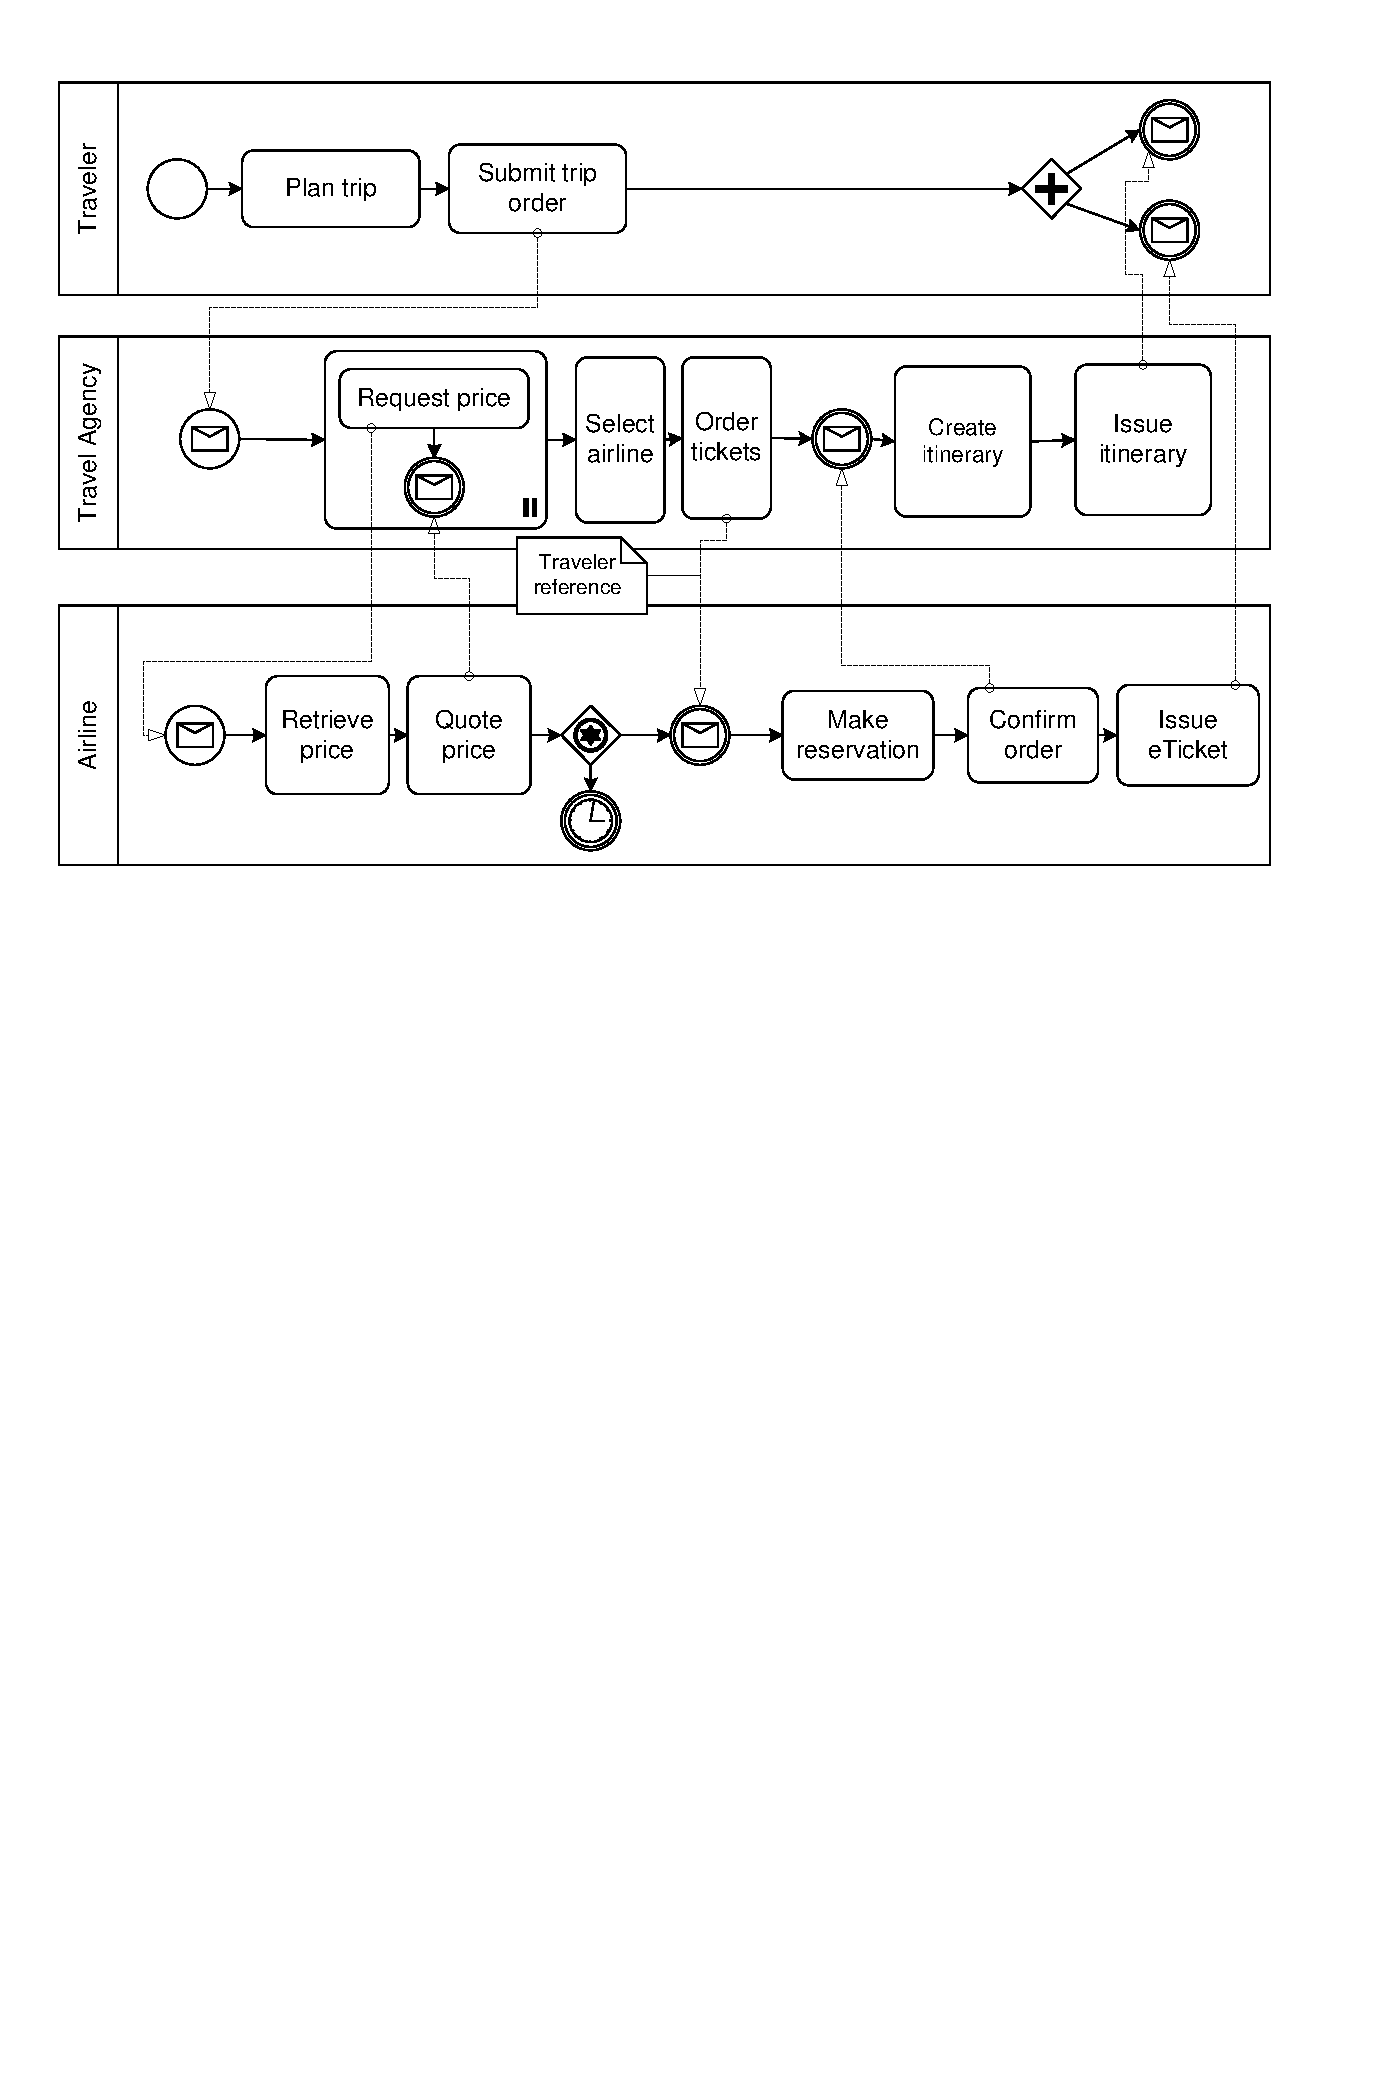
\includegraphics[width=\textwidth]{choreography.pdf}
  \caption{Example Choreography}
  \label{fig:chor1}
\end{figure}

\begin{figure}
  \centering
  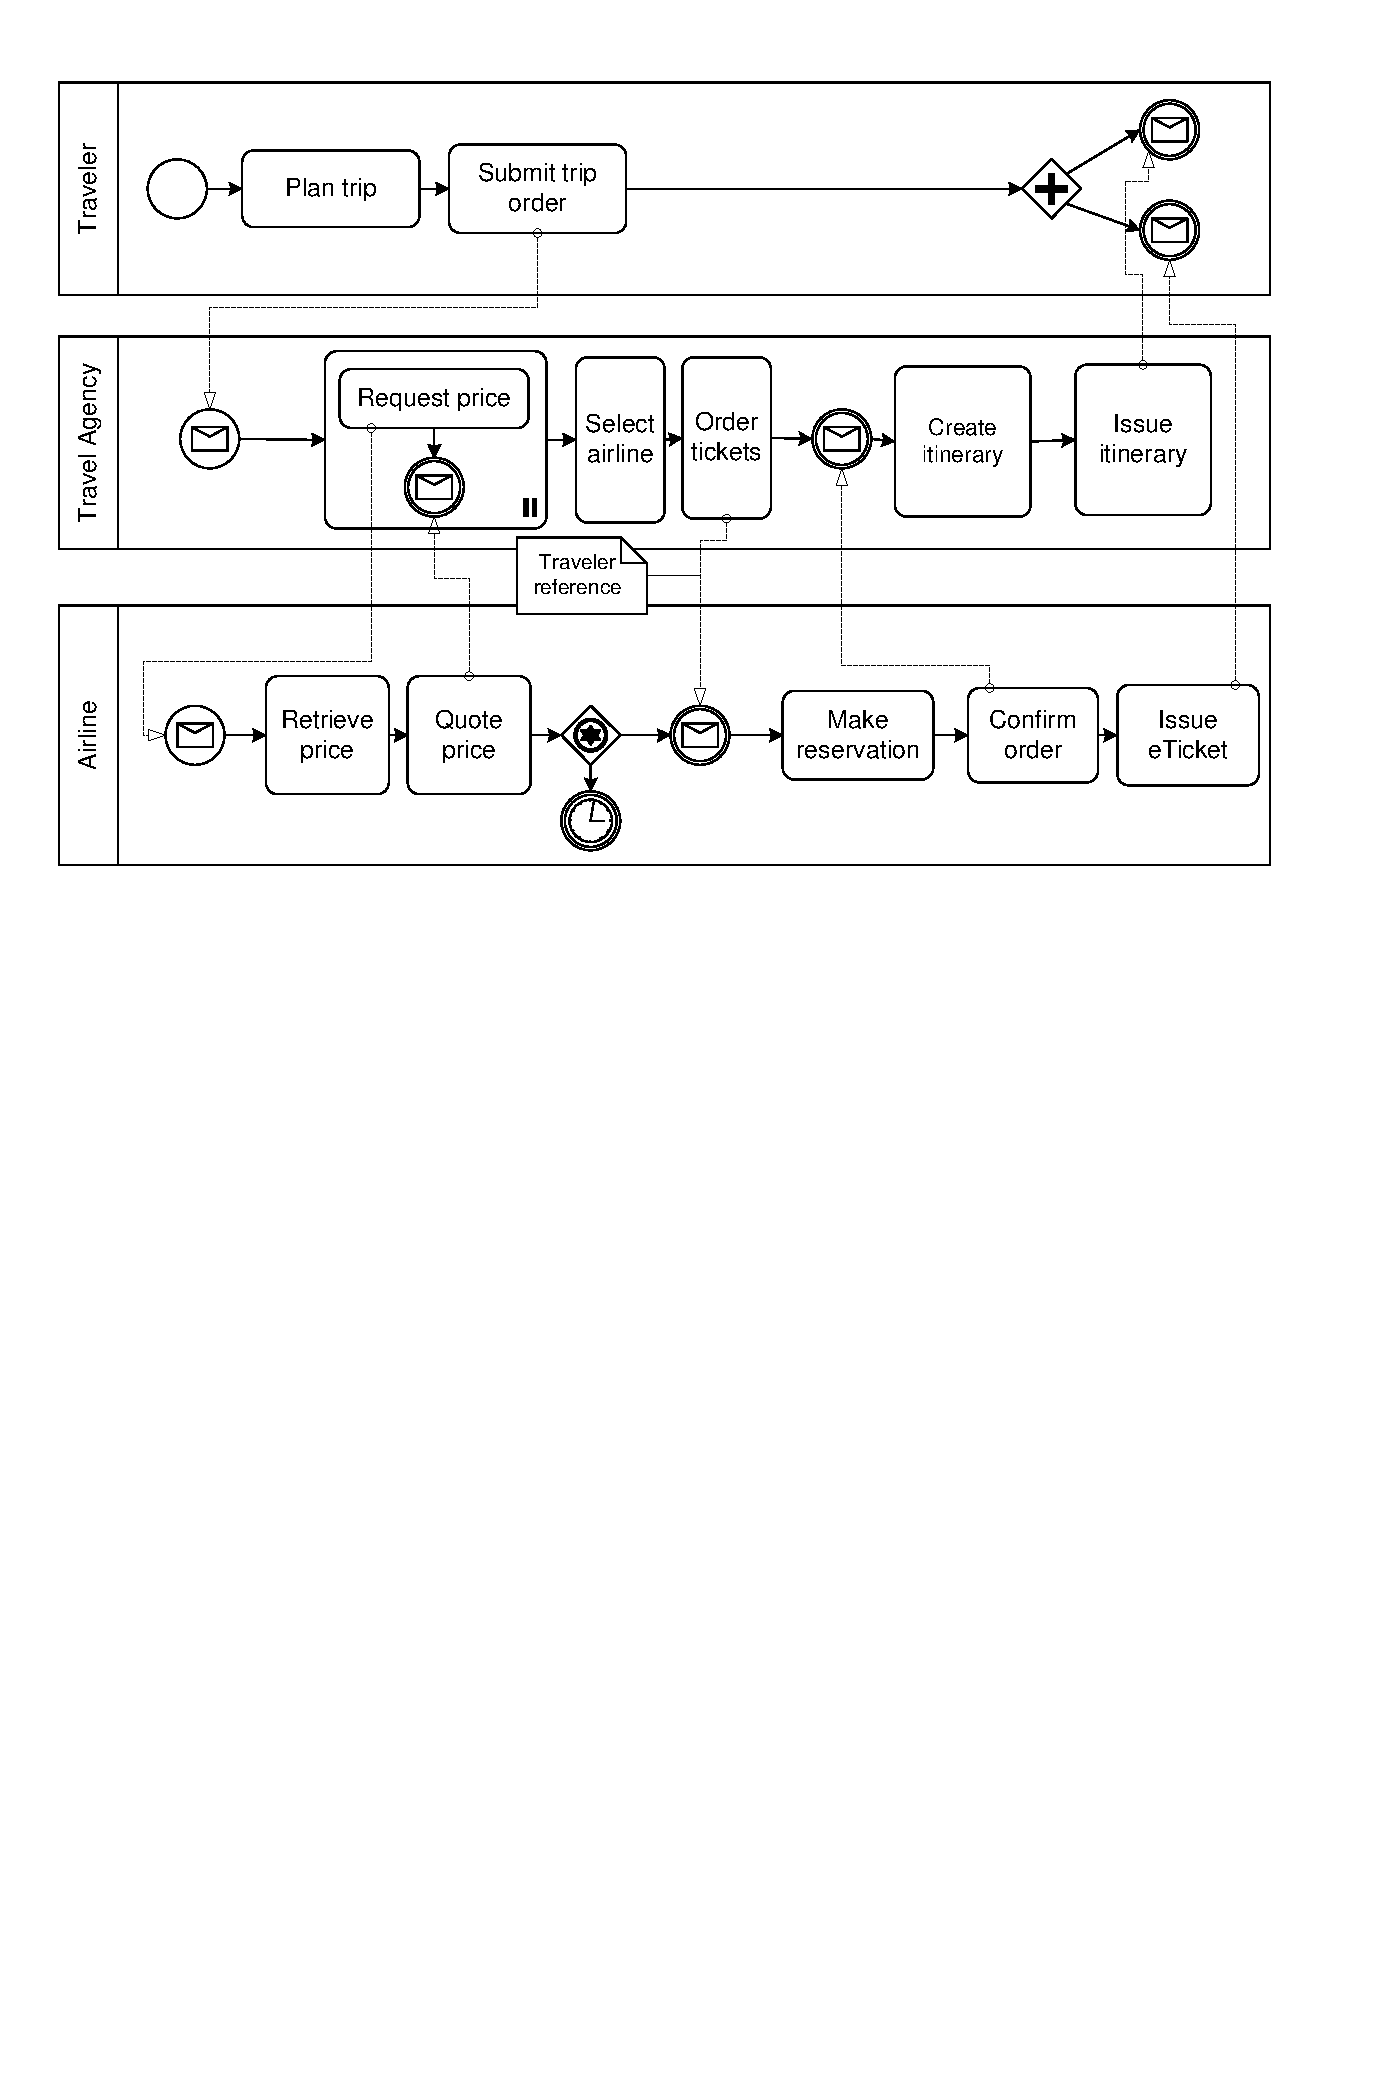
\includegraphics[width=.8\textwidth]{choreography.pdf}
  \caption[Example Choreography]{The example choreography. Now slightly smaller to demonstrate \texttt{\textbackslash textwidth}. And also the use of alternative captions for the list of images. However, the latter is only conditionally recommended, because who reads so much text under a picture? Or is it just a matter of style?}
  \label{fig:chor2}
\end{figure}


\begin{figure}
  \hfill
  \begin{subfigure}{.3\textwidth}
    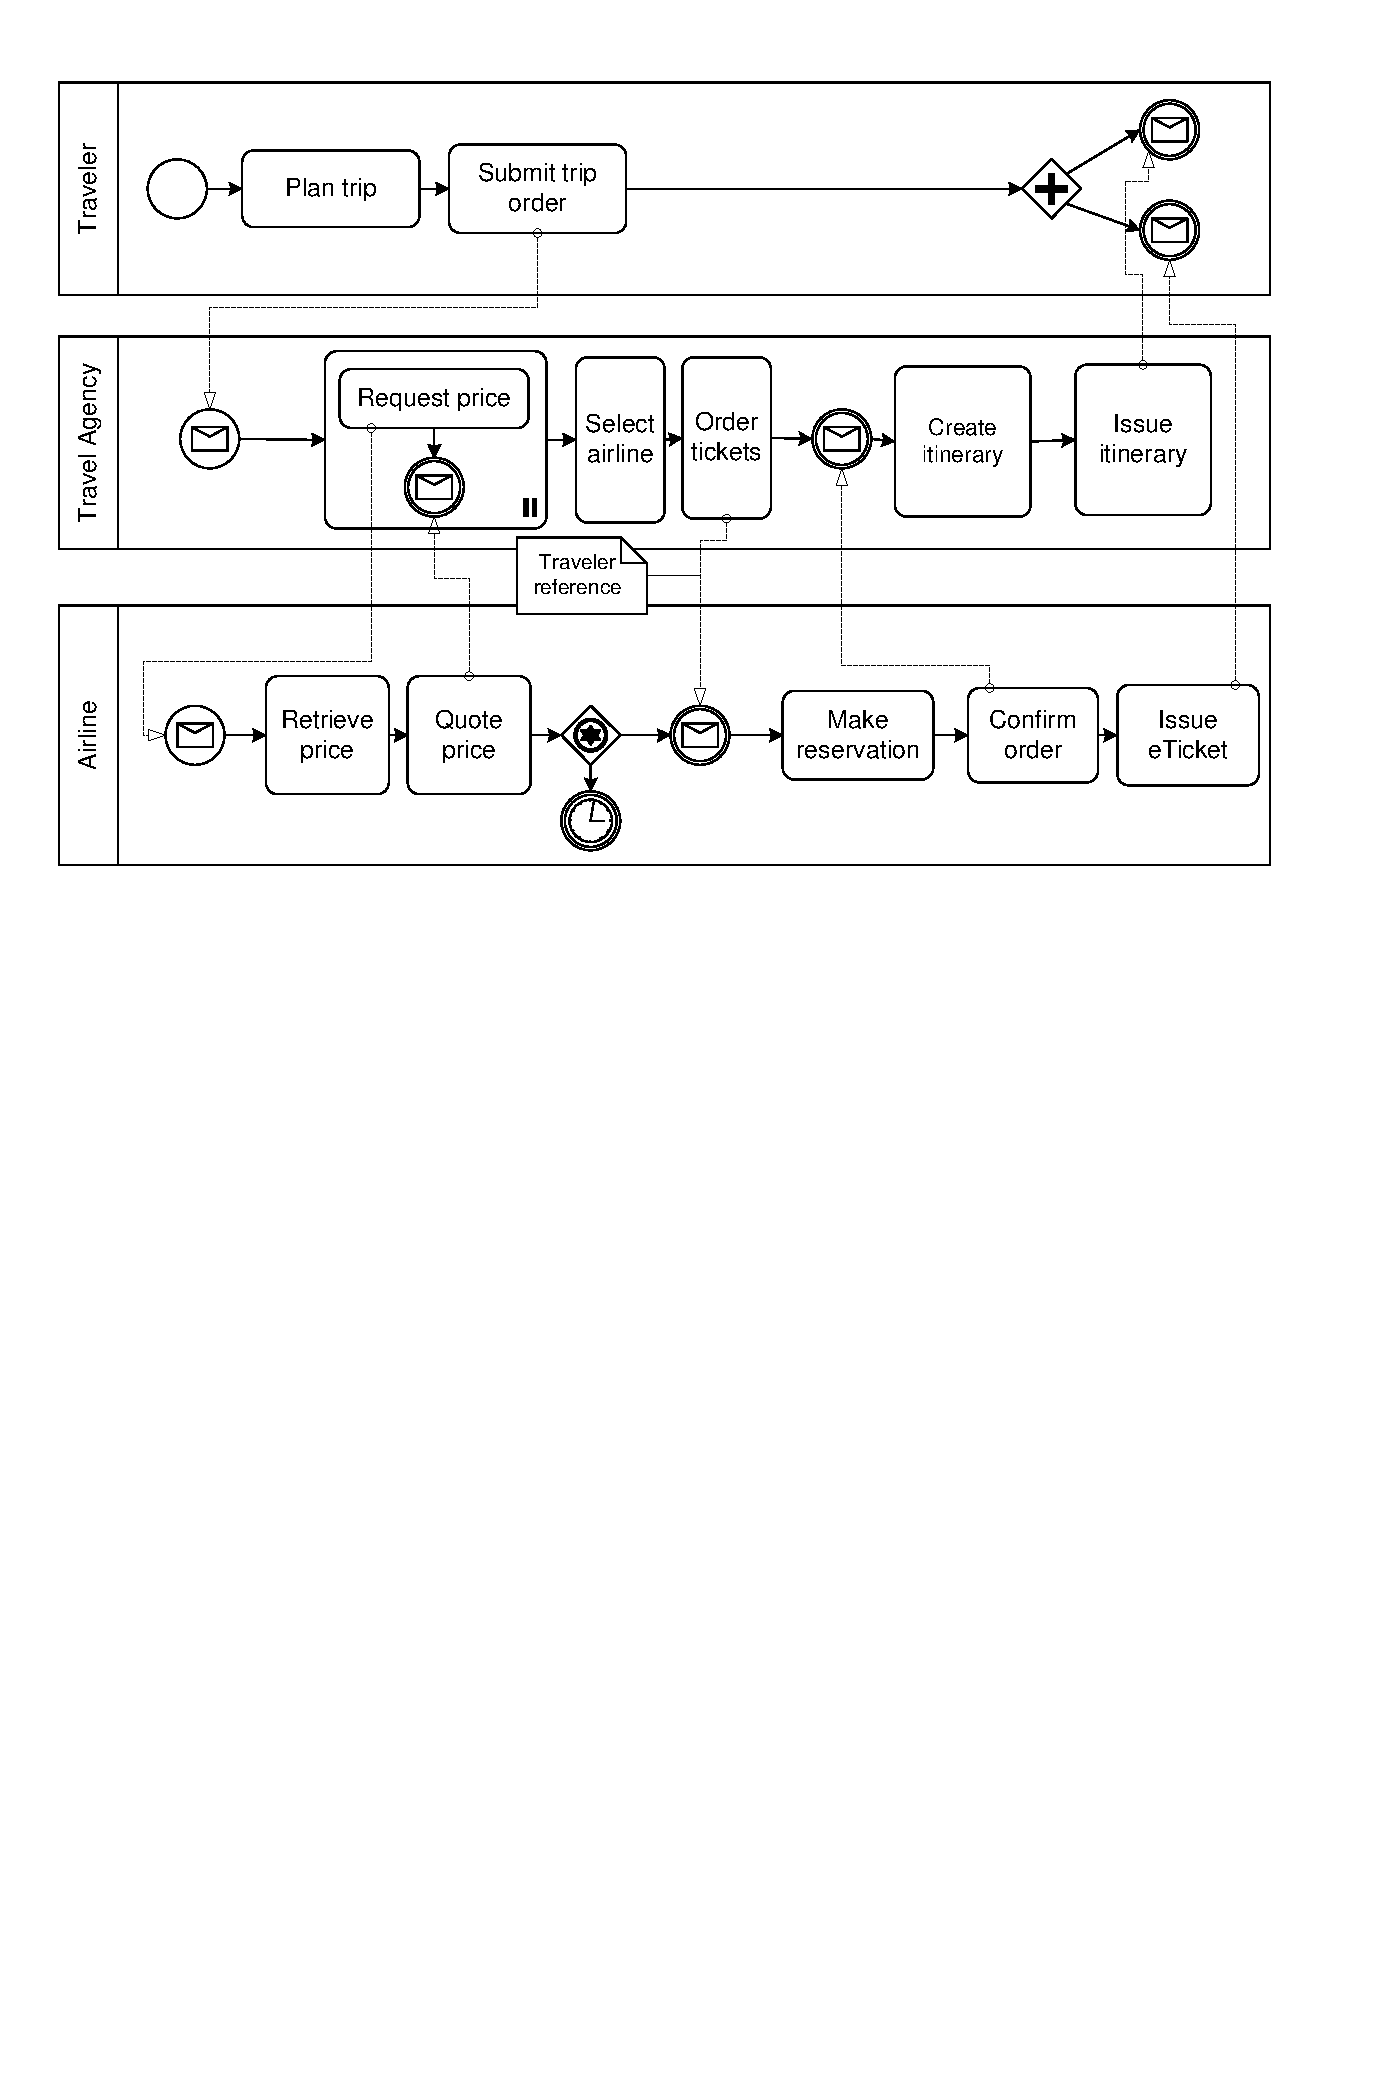
\includegraphics[width=\textwidth]{choreography.pdf}
    \caption{Choreography 1}
    \label{fig:subfigA}
  \end{subfigure}
  \hfill
  \begin{subfigure}{.3\textwidth}
    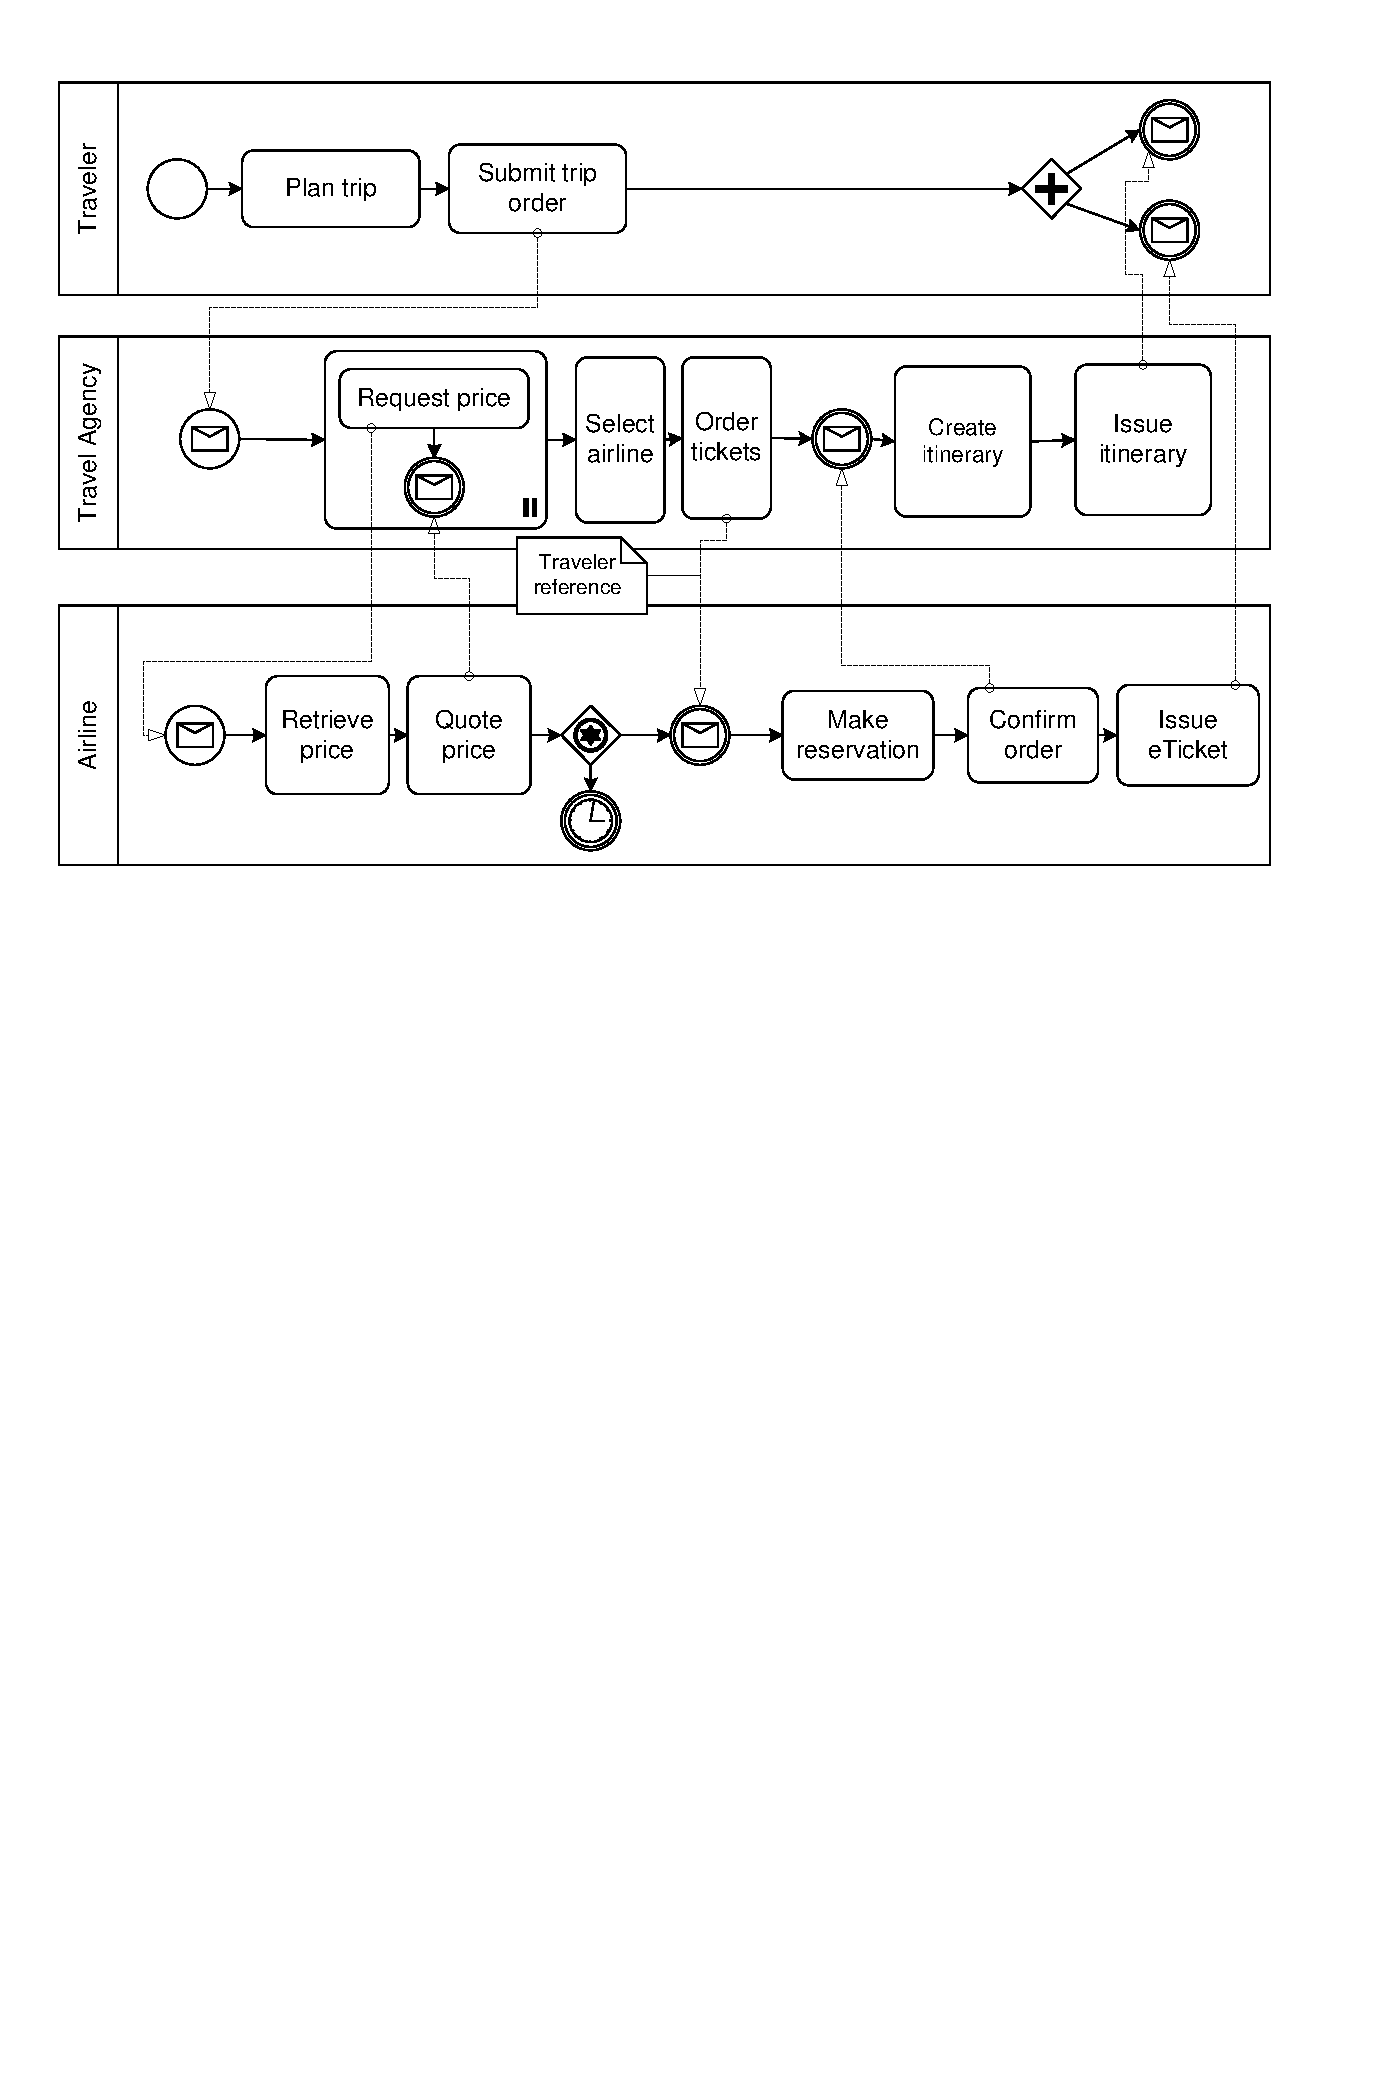
\includegraphics[width=\textwidth]{choreography.pdf}
    \caption{Choreography 2}
    \label{fig:subfigB}
  \end{subfigure}
  \hfill
  \begin{subfigure}{.3\textwidth}
    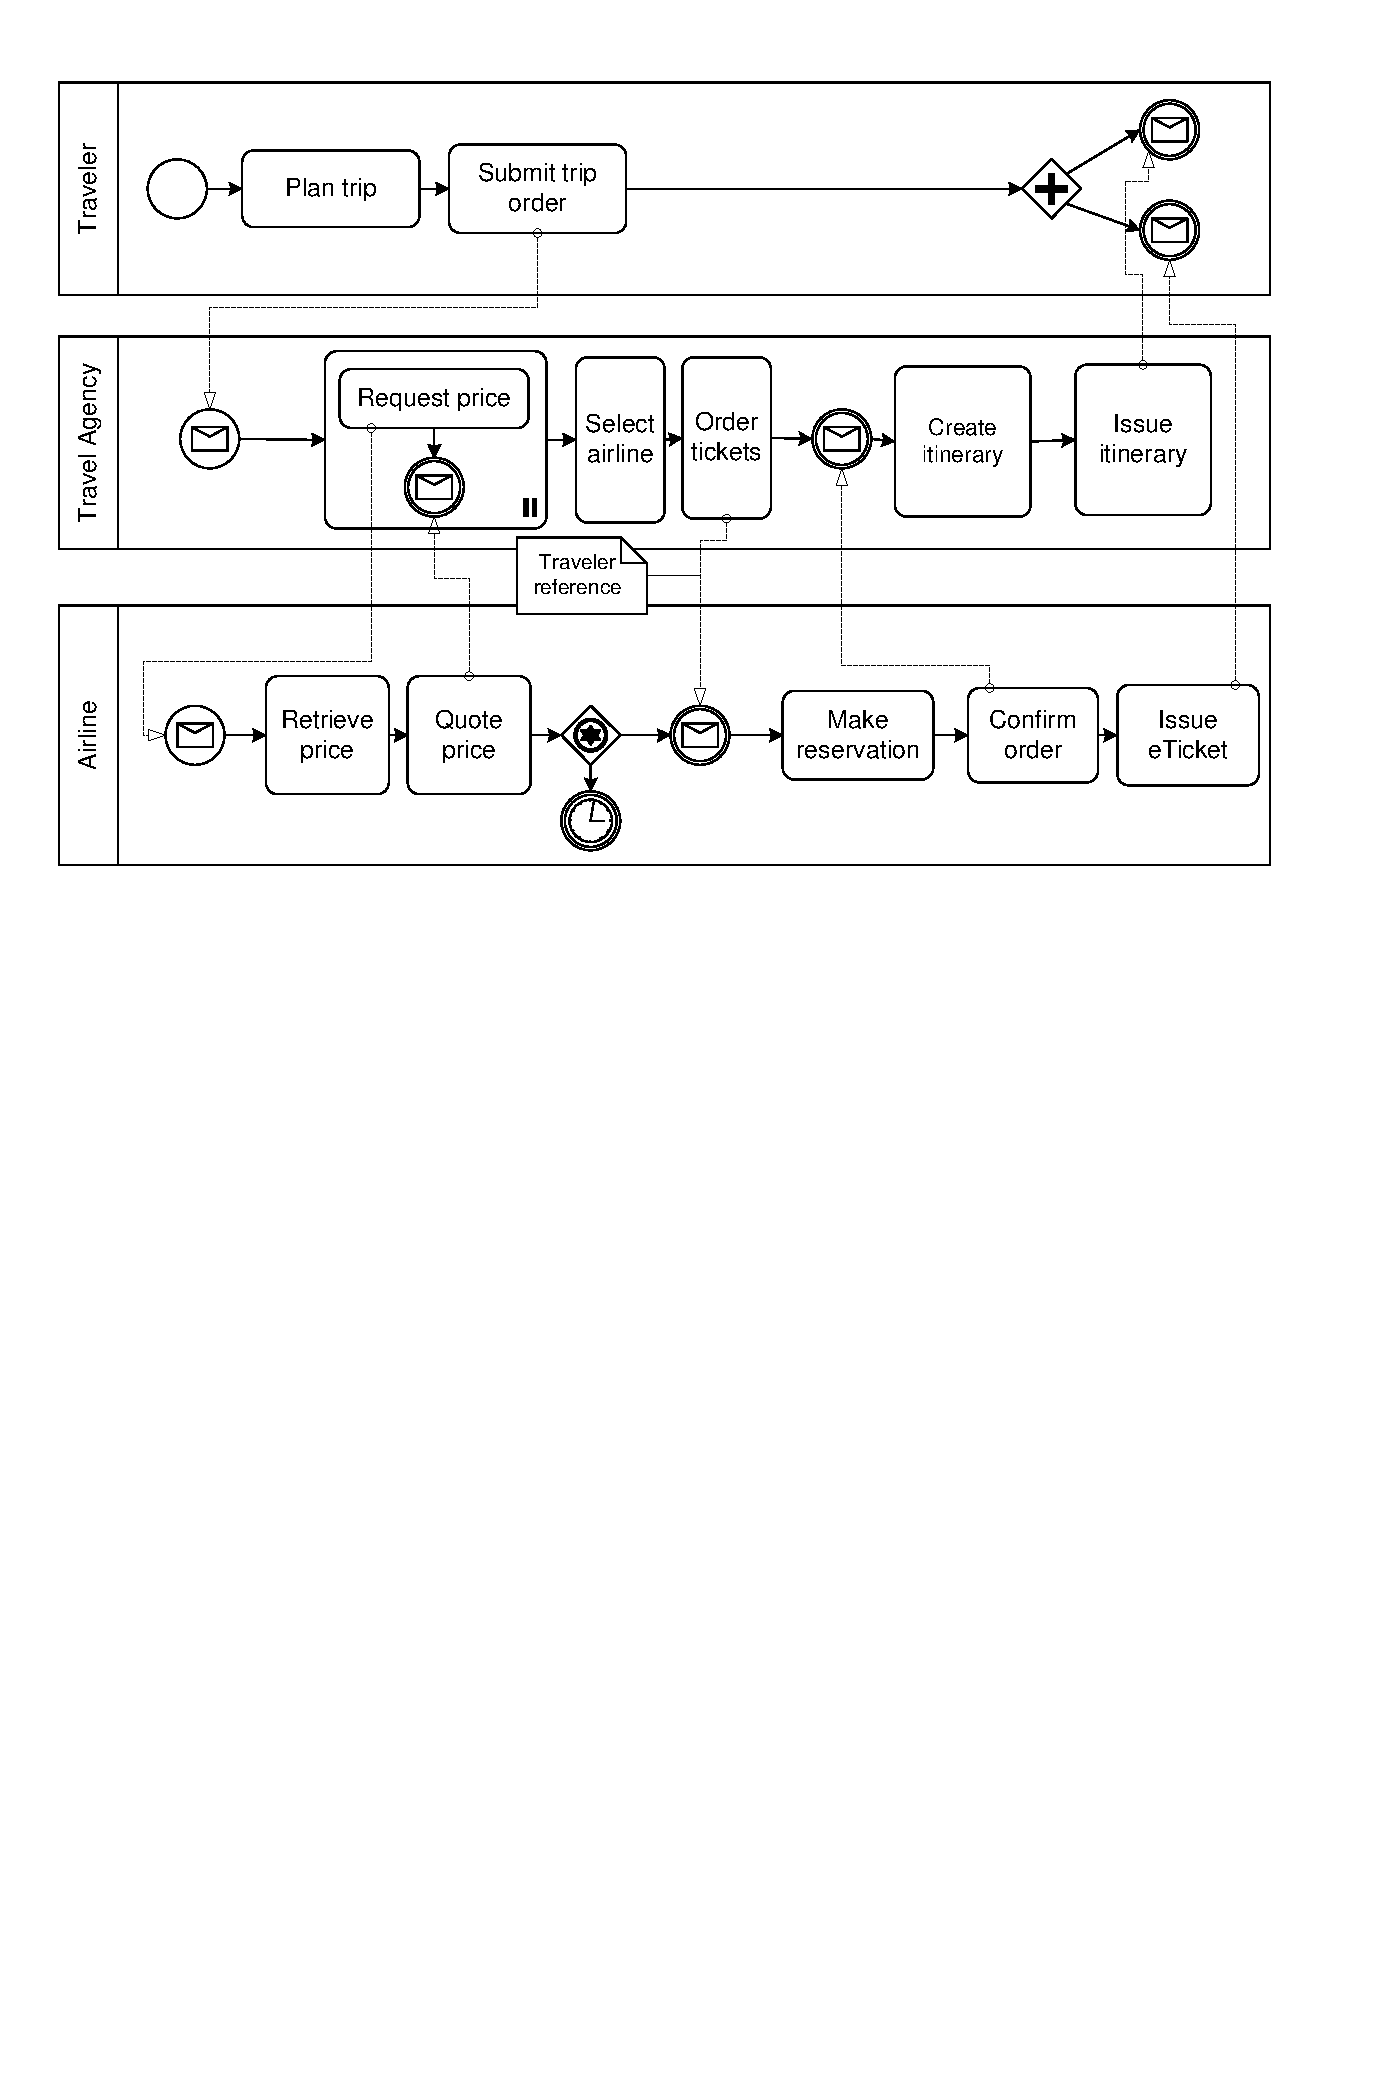
\includegraphics[width=.9\textwidth]{choreography.pdf}
    \caption{Choreography 3}
    \label{fig:subfigC}
  \end{subfigure}
  \caption{Example to place 3 illustrations next to each other. Further, it is possible to reference each separately.}
  \label{fig:subfig_example}
\end{figure}

\Cref{fig:subfig_example} shows the usage of the package subcaption.
It is indeed possible to reference to sub figures: \Cref{fig:subfigA}.

It is possible to convert SVGs to PDF directly during compilation.
This is described in the source code of latex-tipps.tex, but commented out.

\iffalse % <-- Take this away if inkscape is in the path
  The SVG in \cref{fig:directSVG} is directly included, while the text in the SVG in \cref{fig:latexSVG} is set using pdflatex.
  If you want to see the graphics, inkscape must be in PATH and in the text source \texttt{\textbackslash{}iffalse} and \text{\textbackslash{}iftrue} have to be commented out.

  \begin{figure}
    \centering
    
\includegraphics{svgexample.svg}
    \caption{SVG directly included}
    \label{fig:directSVG}
  \end{figure}

  \begin{figure}
    \centering
    \def\svgwidth{.4\textwidth}
    \includesvg{svgexample}
    \caption{Text in SVN set via \LaTeX{}}
    \label{fig:latexSVG}
  \end{figure}
\fi % <-- Take this away if inkscape is in the path



\section{More Illustrations}
\Cref{fig:AnhangsChor,fig:AnhangsChor2} show two choreographies, which should further explain the facts. The second figure is rotated 90 degrees to demonstrate the \texttt{pdflscape} package.

\begin{figure}
  \centering
  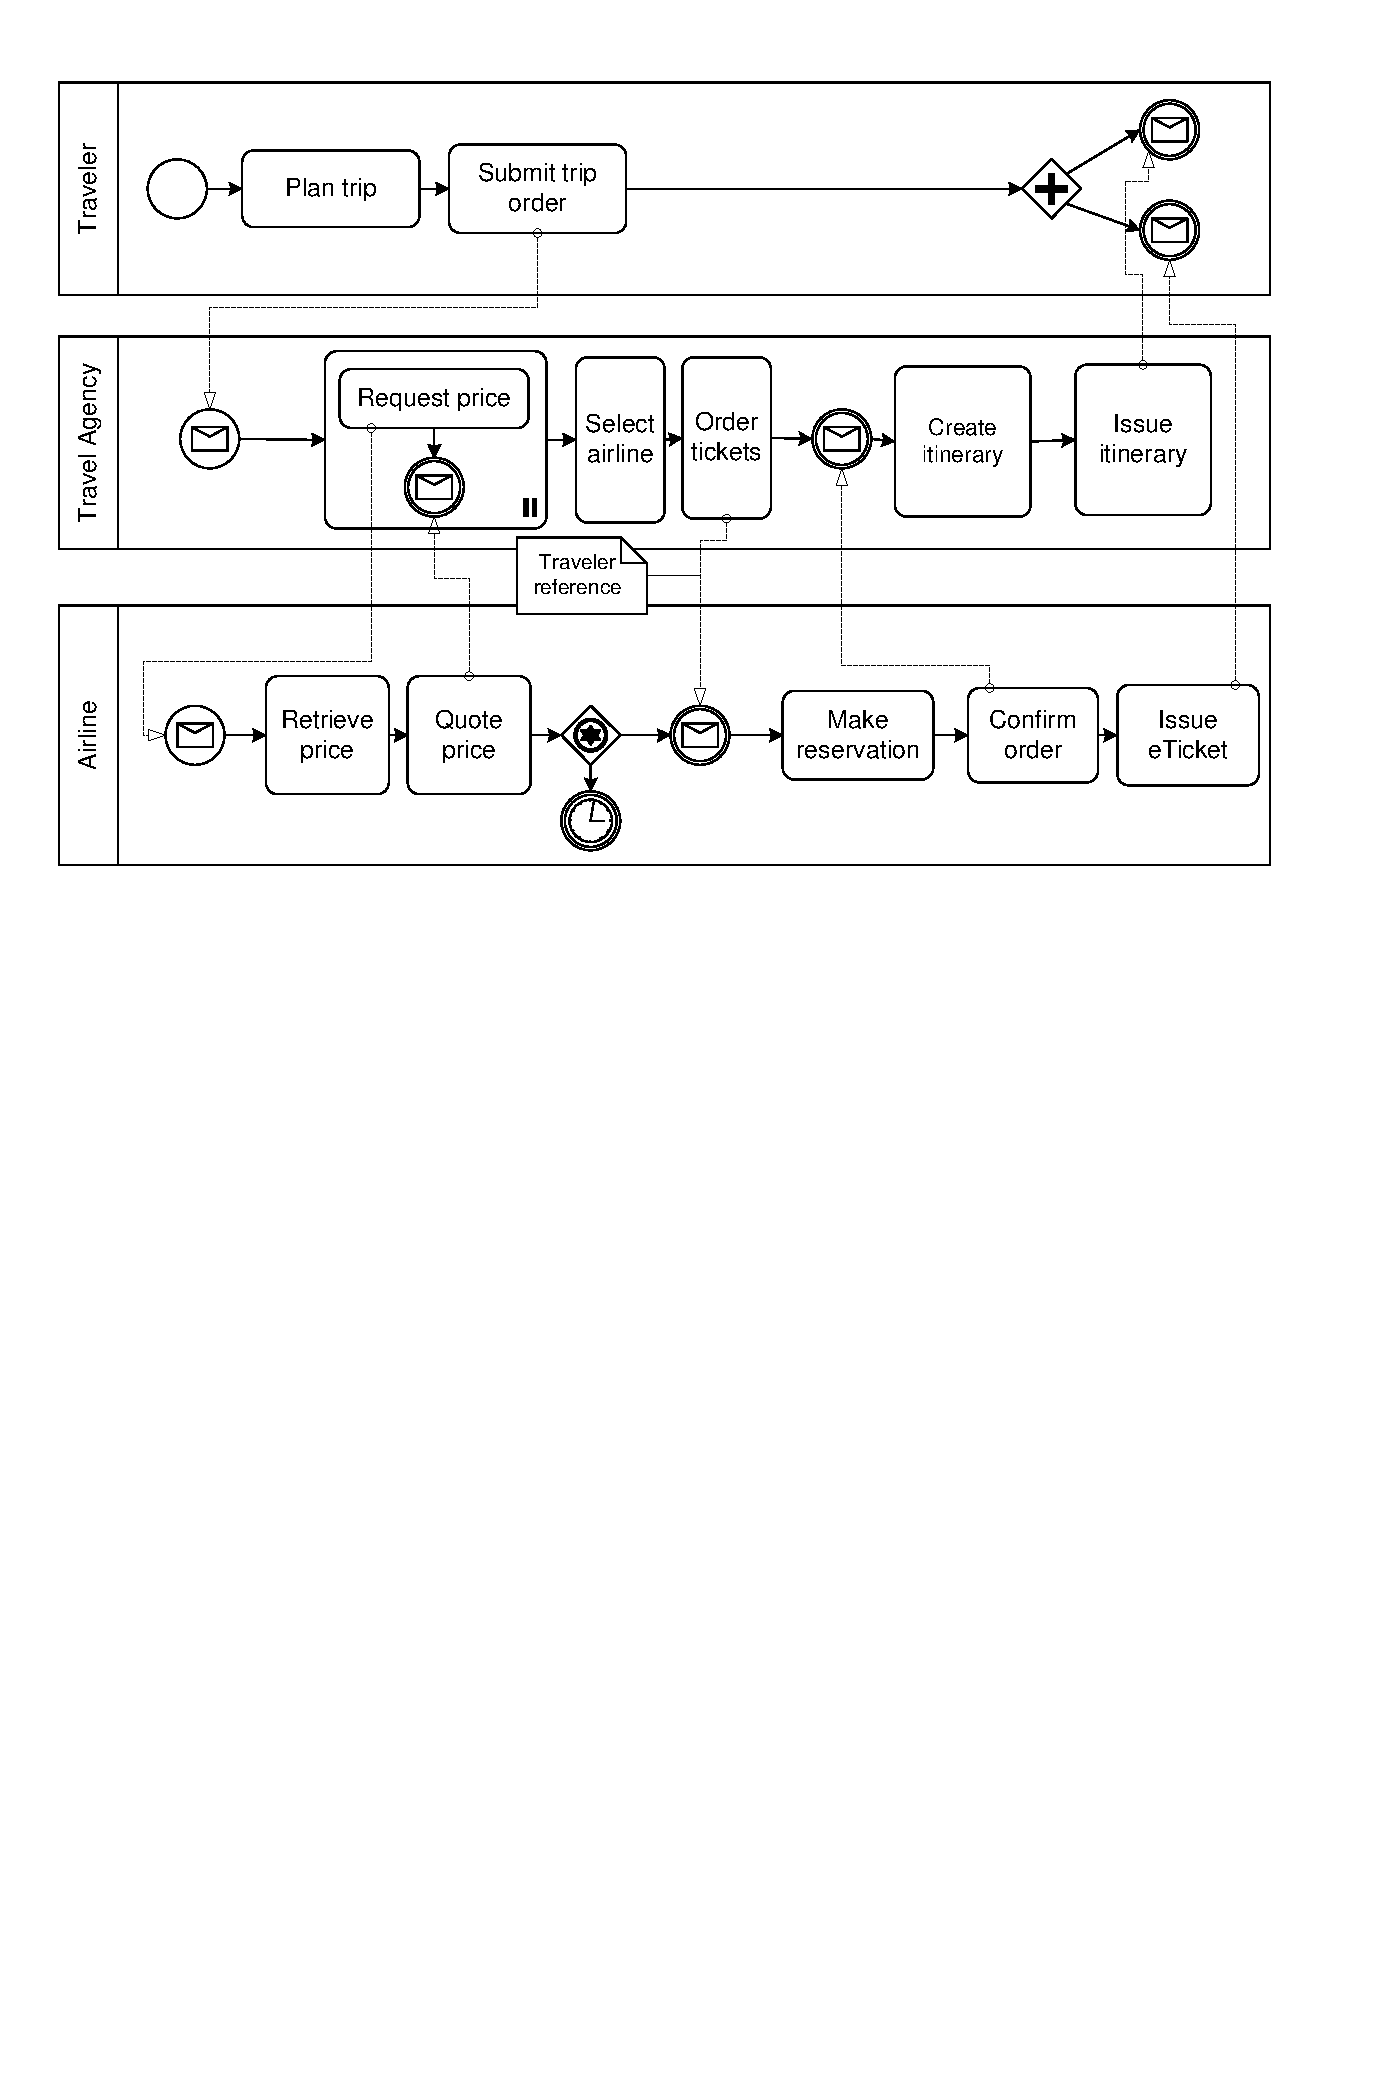
\includegraphics[width=\textwidth]{choreography.pdf}
  \caption{Example Choreography I}
  \label{fig:AnhangsChor}
\end{figure}

\begin{landscape}
  %sidewaysfigure
  \begin{figure}
    \centering
    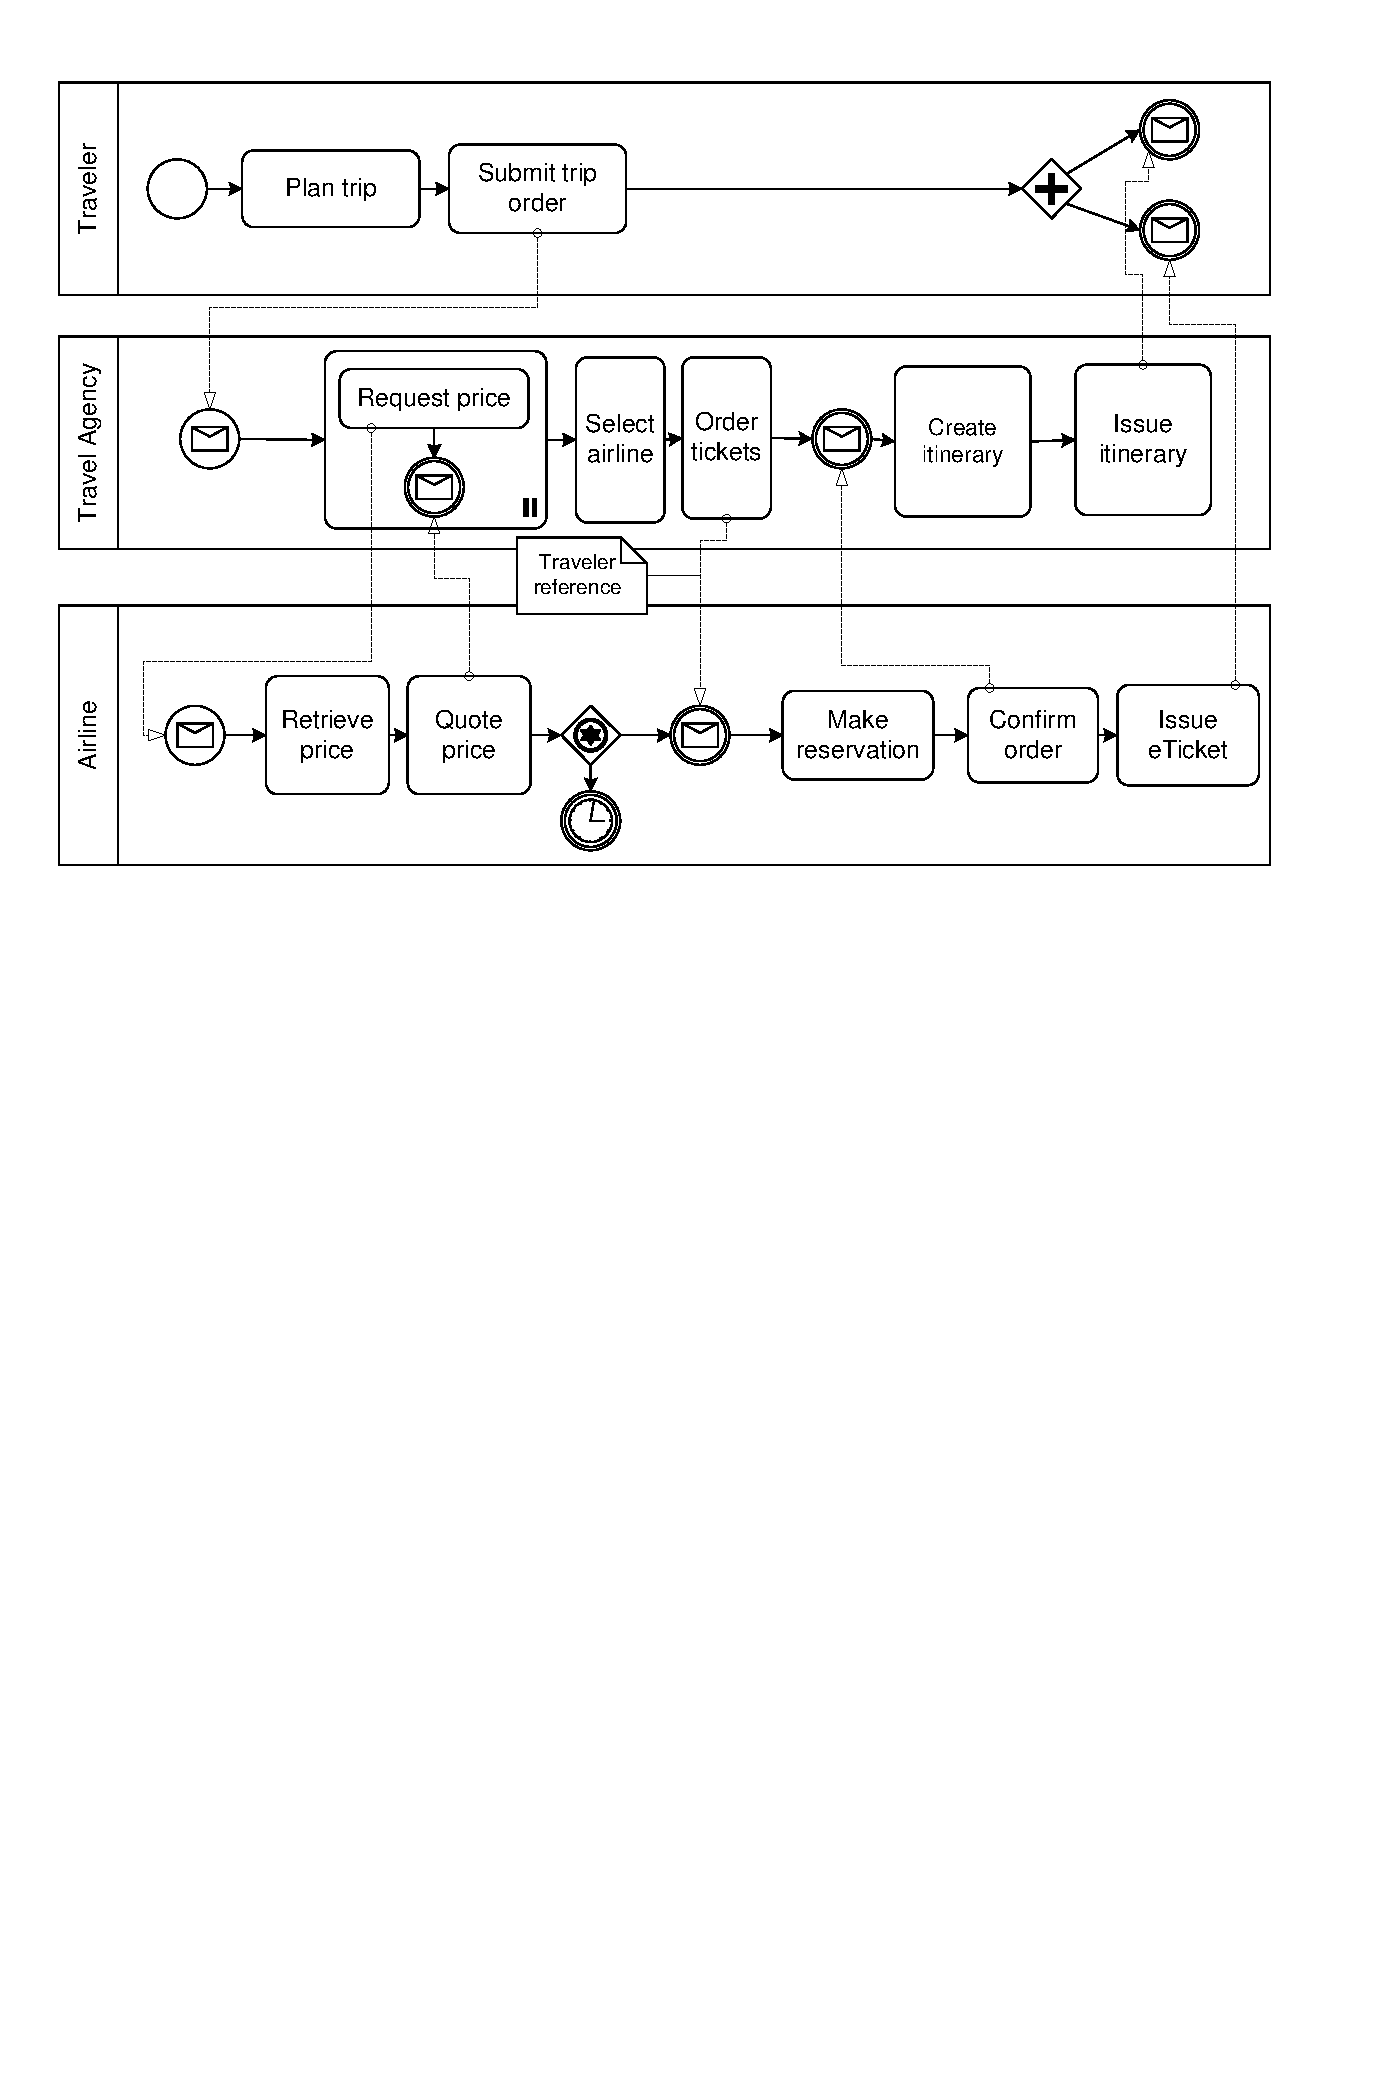
\includegraphics[width=\textwidth]{choreography.pdf}
    \caption{Example Choreography II}
    \label{fig:AnhangsChor2}
  \end{figure}
\end{landscape}


\IfFileExists{pgfplots.sty}{
  %%%%%%%%%%%%%%%%%%%%%%%%%%%%%%%%%%%%%%%%%%%%%%%%%%%%%%%%%%%%%%%%%%%%%%%%%%%%%%
  \section{Plots with pgfplots}
  %%%%%%%%%%%%%%%%%%%%%%%%%%%%%%%%%%%%%%%%%%%%%%%%%%%%%%%%%%%%%%%%%%%%%%%%%%%%%%
  The package pdfplots provides plotting of functions directly in \LaTeX~like with matlab or gnuplot. Some visual examples are available here\footnote{\url{http://texdoc.net/pkg/visualtikz}}.
  \begin{figure}[h]
    \centering
    \begin{tikzpicture}
      \begin{axis}[xlabel=$x$,
          ylabel=$\sin(x)$]
        \addplot {sin(deg(x))};  % Print sine function
      \end{axis}
    \end{tikzpicture}
    \caption{Plot of $\sin(x)$ direclty inside the figure environment with pgfplots.}
  \end{figure}

  \begin{figure}[h]
    \centering
    \begin{tikzpicture}
      \begin{axis}[xlabel=$x$,
          ylabel=$y$]
        \addplot table [x=a, y=c, col sep=comma] {data/data.csv};  % Read coordinates from csv file and plot them
      \end{axis}
    \end{tikzpicture}
    \caption{Coordinates $x$ and $y$ read from csv file and plotted pgfplots.}
  \end{figure}

}{}


%%%%%%%%%%%%%%%%%%%%%%%%%%%%%%%%%%%%%%%%%%%%%%%%%%%%%%%%%%%%%%%%%%%%%%%%%%%%%%
\section{Figures with tikz}
%%%%%%%%%%%%%%%%%%%%%%%%%%%%%%%%%%%%%%%%%%%%%%%%%%%%%%%%%%%%%%%%%%%%%%%%%%%%%%
The tikz is a package for creating graphics programmatically. With this package grids or other regular strucutres can be easliy generated.

\begin{figure}[ht]
  \centering
  \begin{tikzpicture}
    \draw(0,0) rectangle (4,4);
    \foreach \x in {0.5,1,1.5,2,2.5,3,3.5}
    \foreach \y in {0.5,1,1.5,2,2.5,3,3.5}
    \draw(\x,\y) circle (1pt);
  \end{tikzpicture}
  \caption{A regular grid genrated with easily with two for loops.}\label{fig:tikz_example}
\end{figure}


%%%%%%%%%%%%%%%%%%%%%%%%%%%%%%%%%%%%%%%%%%%%%%%%%%%%%%%%%%%%%%%%%%%%%%%%%%%%%%
\section{UML diagrams using tikz-uml}
%%%%%%%%%%%%%%%%%%%%%%%%%%%%%%%%%%%%%%%%%%%%%%%%%%%%%%%%%%%%%%%%%%%%%%%%%%%%%%

\Cref{fig:uml} presents a class diagram typeset using tikz-uml.

\begin{figure}
  \centering
  \begin{tikzpicture}
  \begin{umlpackage}{p}
  \begin{umlpackage}{sp1}
  \umlclass[template=T]{A}{
    n : uint \\ t : float
  }{}
  \umlclass[y=-3]{B}{
    d : double
  }{
    \umlvirt{setB(b : B) : void} \\ getB() : B}
  \end{umlpackage}
  \begin{umlpackage}[x=10,y=-6]{sp2}
  \umlinterface{C}{
    n : uint \\ s : string
  }{}
  \end{umlpackage}
  \umlclass[x=2,y=-10]{D}{
    n : uint
    }{}
  \end{umlpackage}

  \umlassoc[geometry=-|-, arg1=tata, mult1=*, pos1=0.3, arg2=toto, mult2=1, pos2=2.9, align2=left]{C}{B}
  \umlunicompo[geometry=-|, arg=titi, mult=*, pos=1.7, stereo=vector]{D}{C}
  \umlimport[geometry=|-, anchors=90 and 50, name=import]{sp2}{sp1}
  \umlaggreg[arg=tutu, mult=1, pos=0.8, angle1=30, angle2=60, loopsize=2cm]{D}{D}
  \umlinherit[geometry=-|]{D}{B}
  \umlnote[x=2.5,y=-6, width=3cm]{B}{A note with respect to class B}
  \umlnote[x=7.5,y=-2]{import-2}{A anotation}
  \end{tikzpicture}
  \caption{Class diagram generated with tikz-uml. Example adapted from Nicolas Kielbasiewicz.}
  \label{fig:uml}
\end{figure}

\section{UML diagrams using PlantUML}

In case \lualatex{} is used and PlantUML is installed, UML diagrams can be defined using PlantUML.

% Only works if "--shell-escape" is activated. Please activate only if you are sure, your compilation settings are correct
%\IfFileExists{plantuml.sty}{\input{latexhints-english-plantuml}}{}


%%%%%%%%%%%%%%%%%%%%%%%%%%%%%%%%%%%%%%%%%%%%%%%%%%%%%%%%%%%%%%%%%%%%%%%%%%%%%%
\section{Linguistic Forests}
%%%%%%%%%%%%%%%%%%%%%%%%%%%%%%%%%%%%%%%%%%%%%%%%%%%%%%%%%%%%%%%%%%%%%%%%%%%%%%

\begin{filecontents*}[overwrite]{\democodefile}
\begin{forest}
  [VP
    [DP]
    [V’
      [V]
      [DP]
    ]
  ]
\end{forest}
\end{filecontents*}
\PrintDemo{style=parallel}


%%%%%%%%%%%%%%%%%%%%%%%%%%%%%%%%%%%%%%%%%%%%%%%%%%%%%%%%%%%%%%%%%%%%%%%%%%%%%%
\section{Tables}
%%%%%%%%%%%%%%%%%%%%%%%%%%%%%%%%%%%%%%%%%%%%%%%%%%%%%%%%%%%%%%%%%%%%%%%%%%%%%%
\cref{tab:Ergebnisse} shows results and \cref{tab:Werte} shows how numerical data can be represented in a table.
\begin{table}
  \centering
  \begin{tabular}{ccc}
    \toprule
    \multicolumn{2}{c}{\textbf{summed}} & \textbf{Title}                                                          \\ \midrule
    Table                                      & as                                                           & in      \\
    \url{tabsatz.pdf}                            & recommended                                                     & gesetzt \\

    \multirow{2}{*}{Example}                    & \multicolumn{2}{c}{a nice example}                                \\
                                                 & \multicolumn{2}{c}{for using \qq{multirow}}           \\
    \bottomrule
  \end{tabular}
  \caption[Example Table]{Exampe Table -- see \url{http://www.ctan.org/tex-archive/info/german/tabsatz/}}
  \label{tab:Ergebnisse}
\end{table}

\begin{table}
  \centering
  \begin{tabular}{l *{8}{d{3.2}}}
    \toprule

                         & \multicolumn{2}{c}{\textbf{Parameter 1}} & \multicolumn{2}{c}{\textbf{Parameter 2}} & \multicolumn{2}{c}{\textbf{Parameter 3}} & \multicolumn{2}{c}{\textbf{Parameter 4}}                                                                                                                                       \\
    \cmidrule(r){2-3}\cmidrule(lr){4-5}\cmidrule(lr){6-7}\cmidrule(l){8-9}

    \textbf{Bedingungen} & \multicolumn{1}{c}{\textbf{M}}           & \multicolumn{1}{c}{\textbf{SD}}          & \multicolumn{1}{c}{\textbf{M}}           & \multicolumn{1}{c}{\textbf{SD}}          & \multicolumn{1}{c}{\textbf{M}} & \multicolumn{1}{c}{\textbf{SD}} & \multicolumn{1}{c}{\textbf{M}} & \multicolumn{1}{c}{\textbf{SD}} \\
    \midrule

    W                    & 1.1                                      & 5.55                                     & 6.66                                     & .01                                      &                                &                                 &                                &                                 \\
    X                    & 22.22                                    & 0.0                                      & 77.5                                     & .1                                       &                                &                                 &                                &                                 \\
    Y                    & 333.3                                    & .1                                       & 11.11                                    & .05                                      &                                &                                 &                                &                                 \\
    Z                    & 4444.44                                  & 77.77                                    & 14.06                                    & .3                                       &                                &                                 &                                &                                 \\
    \bottomrule
  \end{tabular}

  \caption{Example table for 4 constraints (W-Z), each having 4 parameters with (M und SD). Note: use always the same number of decimal places.}
  \label{tab:Werte}
\end{table}

\IfFileExists{pgfplotstable.sty}{

\subsection{Tables with pgfplots}
With the pgfplotstable package tables can be directly generated from a csv file.

\begin{table}[h]
\centering
\pgfplotstabletypeset[
col sep = comma,
every head row/.style={before row=\toprule,after row=\midrule},
every last row/.style={after row=\bottomrule},
display columns/0/.style={string type,column name={}}
]
{data/data.csv}
\caption{Table direclty generated from the values of a csf file.}
\end{table}
}{}


\section{Tables spanning multiple pages}


\begin{longtable}{|l|l|l|}
\caption{A sample long table.} \label{tab:long} \\

\hline \multicolumn{1}{|c|}{\textbf{First column}} & \multicolumn{1}{c|}{\textbf{Second column}} & \multicolumn{1}{c|}{\textbf{Third column}} \\ \hline
\endfirsthead

\multicolumn{3}{c}%
{{\bfseries \tablename\ \thetable{} -- continued from previous page}} \\
\hline \multicolumn{1}{|c|}{\textbf{First column}} & \multicolumn{1}{c|}{\textbf{Second column}} & \multicolumn{1}{c|}{\textbf{Third column}} \\ \hline
\endhead

\hline \multicolumn{3}{|r|}{{Continued on next page}} \\ \hline
\endfoot

\hline \hline
\endlastfoot

A & BC & D \\
A & BC & D \\
A & BC & D \\
A & BC & D \\
A & BC & D \\
A & BC & D \\
A & BC & D \\
A & BC & D \\
A & BC & D \\
A & BC & D \\
A & BC & D \\
A & BC & D \\
A & BC & D \\
A & BC & D \\
A & BC & D \\
A & BC & D \\
A & BC & D \\
A & BC & D \\
A & BC & D \\
A & BC & D \\
A & BC & D \\
A & BC & D \\
A & BC & D \\
A & BC & D \\
A & BC & D \\
A & BC & D \\
A & BC & D \\
A & BC & D \\
A & BC & D \\
A & BC & D \\
A & BC & D \\
A & BC & D \\
A & BC & D \\
A & BC & D \\
A & BC & D \\
A & BC & D \\
A & BC & D \\
A & BC & D \\
A & BC & D \\
A & BC & D \\
A & BC & D \\
A & BC & D \\
A & BC & D \\
A & BC & D \\
A & BC & D \\
A & BC & D \\
A & BC & D \\
A & BC & D \\
A & BC & D \\
A & BC & D \\
A & BC & D \\
A & BC & D \\
A & BC & D \\
A & BC & D \\
A & BC & D \\
A & BC & D \\
A & BC & D \\
A & BC & D \\
A & BC & D \\
A & BC & D \\
A & BC & D \\
A & BC & D \\
A & BC & D \\
A & BC & D \\
A & BC & D \\
A & BC & D \\
A & BC & D \\
A & BC & D \\
A & BC & D \\
A & BC & D \\
A & BC & D \\
A & BC & D \\
A & BC & D \\
A & BC & D \\
A & BC & D \\
A & BC & D \\
A & BC & D \\
A & BC & D \\
A & BC & D \\
A & BC & D \\
\end{longtable}


%%%%%%%%%%%%%%%%%%%%%%%%%%%%%%%%%%%%%%%%%%%%%%%%%%%%%%%%%%%%%%%%%%%%%%%%%%%%%%
\section{Abbreviations}
%%%%%%%%%%%%%%%%%%%%%%%%%%%%%%%%%%%%%%%%%%%%%%%%%%%%%%%%%%%%%%%%%%%%%%%%%%%%%%
At the first pass the \gls{fr} was 5.
At the second pass was \gls{fr} 3.
The plural form can be seen here: \glspl{er}.
To demonstrate what the list of abbreviations looks like for longer description texts, \glspl{rdbms} must be mentioned here.

With \verb+\gls{...}+ you can enter abbreviations, the first time you call it, the long form is used.
When reusing \verb+\gls{..}+ the short form is automatically displayed.
The abbreviation is also automatically inserted in the abbreviation list.
With \verb+\glspl{...}+ the plural form is used.
If you want the short form to appear directly at the first use, you can use \verb+\glsunset{..}+ to mark an abbreviation as already used.
The opposite is achieved with \verb+\glsreset{..}+.

Abbreviations are defined in \verb+\content\ausarbeitung.tex+ by means of \verb+\newacronym{...}{...}{...}+.

More information at: \url{http://tug.ctan.org/macros/latex/contrib/glossaries/glossariesbegin.pdf}
%%%%%%%%%%%%%%%%%%%%%%%%%%%%%%%%%%%%%%%%%%%%%%%%%%%%%%%%%%%%%%%%%%%%%%%%%%%%%%
\section{References}
%%%%%%%%%%%%%%%%%%%%%%%%%%%%%%%%%%%%%%%%%%%%%%%%%%%%%%%%%%%%%%%%%%%%%%%%%%%%%%
For distant sections \qq{varioref} is recommended:
\qq{See \vref{sec:mf}}.
The command \texttt{\textbackslash{}vref} works similar to \texttt{\textbackslash{}cref} the difference beeing that a reference to the page is additionally added.
\texttt{vref}: \qq{\vref{sec:firstsectioninlatexhints}}, \texttt{cref}: \qq{\cref{sec:firstsectioninlatexhints}}, \texttt{ref}: \qq{\ref{sec:firstsectioninlatexhints}}.

If \qq{varioref} causes difficulties, then \qq{cref} can be used instead.
This also creates the word \qq{section} automatically: \cref{sec:mf}.
This is also possible for illustrations etc.
In English please use \verb1\Cref{...}1 (with large \qq{C} at the beginning).

%With MiKTeX installation from 2012-01-16 no longer necessary.
%If a section becomes longer than one page and you want to refer to a specific place in the section with \texttt{\textbackslash{}vref}, then you should use \texttt{\textbackslash{}phantomsection} then using \texttt{vref} will also display the correct page number.

%%The link location will be placed on the line below.
%%Tipp von http://en.wikibooks.org/wiki/LaTeX/Labels_and_Cross-referencing#The_hyperref_package_and_.5Cphantomsection
%\phantomsection
%\label{alabel}
%View the example for \texttt{\textbackslash{}phantomsection} in the \LaTeX{} source code.

%Here is the example: See Section \vref{hack1} and Section \vref{hack2}.
%%%%%%%%%%%%%%%%%%%%%%%%%%%%%%%%%%%%%%%%%%%%%%%%%%%%%%%%%%%%%%%%%%%%%%%%%%%%%%
\section{Definitions}
%%%%%%%%%%%%%%%%%%%%%%%%%%%%%%%%%%%%%%%%%%%%%%%%%%%%%%%%%%%%%%%%%%%%%%%%%%%%%%
\begin{definition}[Title]
  \label{def:def1}
  Definition Text
\end{definition}

\Cref{def:def1} shows \ldots

%%%%%%%%%%%%%%%%%%%%%%%%%%%%%%%%%%%%%%%%%%%%%%%%%%%%%%%%%%%%%%%%%%%%%%%%%%%%%%
\section{Footnotes}
%%%%%%%%%%%%%%%%%%%%%%%%%%%%%%%%%%%%%%%%%%%%%%%%%%%%%%%%%%%%%%%%%%%%%%%%%%%%%%
Footnotes are provided by the command \verb+\footnote{...}+\footnote{\label{fussnote}Example footnote.}. Citing footnotes is possible by provinding a label\verb+\footnote{\label{...}...}+ and cite the footnote with \verb+\cref{...}+ in the text\cref{fussnote}.
%%%%%%%%%%%%%%%%%%%%%%%%%%%%%%%%%%%%%%%%%%%%%%%%%%%%%%%%%%%%%%%%%%%%%%%%%%%%%%

%%%%%%%%%%%%%%%%%%%%%%%%%%%%%%%%%%%%%%%%%%%%%%%%%%%%%%%%%%%%%%%%%%%%%%%%%%%%%%
\section{Various Things}
%%%%%%%%%%%%%%%%%%%%%%%%%%%%%%%%%%%%%%%%%%%%%%%%%%%%%%%%%%%%%%%%%%%%%%%%%%%%%%
\label{sec:diff}
\ifdeutsch
  Numbers (123\,654\,789) are nicely set.
  Either in a line or as non-lining figure.
  The latter is reached by parameter \texttt{osf} at package \texttt{libertine} or.\ \texttt{mathpazo} in \text{fonts.tex}.
\fi

\begin{filecontents*}[overwrite]{\democodefile}
\begin{compactenum}[I.]
  \item You can also keep the numbering compact thanks to paralist
  \item and switch to a different numbering
\end{compactenum}
\end{filecontents*}
\PrintDemo{style=parallel}

The words \qq{workflow} and \qq{dwarflike} can be copied from the PDF and pasted to a text file.

\begin{filecontents*}[overwrite]{\democodefile}
In case \LuaLaTeX{} is used as compiler, there is no ligature at \qq{f\/l} in the word \qq{dwarflike} (in contrast to \qq{fl} at \qq{workflow}).
In other words: \qq{dwarflike} and \qq{dwarf\/like} look the same in the PDF.
In case they do not, there is an issue with Lua\LaTeX{} and the selnolig package.
\end{filecontents*}
\PrintDemo{style=parallel}
% Meta comment: The precise form of the optimal ligation suppression command may vary depending on the character pairs involved - see https://tex.stackexchange.com/q/28437/9075


%%%%%%%%%%%%%%%%%%%%%%%%%%%%%%%%%%%%%%%%%%%%%%%%%%%%%%%%%%%%%%%%%%%%%%%%%%%%%%
\section{Closing remarks}
%%%%%%%%%%%%%%%%%%%%%%%%%%%%%%%%%%%%%%%%%%%%%%%%%%%%%%%%%%%%%%%%%%%%%%%%%%%%%%
Please feel free to provide enhancements for this template and create a new ticket on GitHub (\url{https://github.com/latextemplates/uni-stuttgart-computer-science-template/issues}).

\chapter{Appendix}
In this Appendix we provide supplementary information to complement the preceding chapters of our thesis. 
Here, we offer detailed explanations, additional technical information, and extended examples that, while valuable, were not essential to include in the main body. 
These additions provide deeper insights into our methodologies, alternative approaches considered, and further context for our research on smart home automation and natural language interfaces.

\section{Training a Large Language Model for Smart Home Automation}
\label{sec:relatedwork-appendix}
\begin{Listing}[bh]
    \begin{lstlisting}
      <|system|>You are 'Al', a helpful AI Assistant that controls the devices in a house. Complete the following task as instructed or answer the following question with the information provided only.
      The current time and date is 08:12 AM on Thursday March 14, 2024
      
      Services: light.turn_off(), light.turn_on(rgb_color,brightness), fan.turn_on(), fan.turn_off()
      
      Devices:
      light.office 'Office Light' = on;80%
      fan.office 'Office fan' = off
      light.kitchen 'Kitchen Light' = on;80%;red
      light.bedroom 'Bedroom Light' = off<|endoftext|>
      
      <|user|>
      please turn on the lights in the kitchen now<|endoftext|>
  
      <|assistant|>I'll turn the lights on for you right way
      ```homeassistant
      { "service": "light.turn_on", "target_device": "light.kitchen" }
      ```<|endoftext|>
    \end{lstlisting}
    \caption{Example Format for Training a Large Language Model on Smart Home Control}
    \label{lst:homeLLM}
  \end{Listing}
The owner of the Home LLM repository \cite{acon96_home_llm} provided us insights on how to build a model similar to his upon request.
Even if our intention is not on fine-tuning an LLM, such information can be very helpful, for example to get inspired by the training data format. 
The primary focus in the process is on constructing a comprehensive dataset that represents various scenarios where a personal assistant interacts with Home Assistant. This dataset, which forms the core of the project, consists of thousands of examples demonstrating different interactions, such as controlling devices or responding to user queries.
The dataset is formatted to include all necessary information for the model to understand and execute tasks. An example format might look like \cref{lst:homeLLM}

Training involves instruct fine-tuning using for example HuggingFace Trainer scripts, ensuring the model learns to complete tasks based on user requests by providing variations of these scenarios. Critical steps include matching the model's instruct/chat format, masking out the context during training, and fine-tuning hyper-parameters like learning rate and training schedule.
An evaluation framework is essential to measure model accuracy and compare training runs, ensuring effective model performance.


\section{Additional Intents}
\label{sec:intents-appendix}
This supplementary section explains additional Intents to the ones described in \cref{sec:intent-eng} that we were not able to implement.
\subsection{Iteration 2: Intermediate Intents}

\paragraph{Assistance for Creating Automations}

\begin{itemize}
    \item \textbf{Intent Name:} CreateAutomation
    \item \textbf{Examples:}
    \begin{itemize}
        \item ``Set up an automation for turning off lights at 10 PM.''
        \item ``Create a rule to adjust thermostat settings when I leave home.''
        \item ``Can you help me with automating my smart blinds?''
        \item ``Notify me if any windows are open.''
    \end{itemize}
    \item \textbf{Entities:}
    \begin{itemize}
        \item DeviceType (e.g., lights, thermostat, blinds)
        \item TriggerEvent (e.g., time-based, occupancy, temperature change)
        \item Condition (optional, e.g., specific temperature threshold)
        \item Action (e.g., turn off, adjust settings)
        \item Location (optional, e.g., living room, bedroom)
    \end{itemize}
    \item \textbf{Action/Response:} Assisting the user in defining and setting up a smart home automation, including specifying the devices involved, the triggering event, any conditions, and the desired actions. The chatbot may also provide suggestions for common automation scenarios.
\end{itemize}

Creating automations is a common use case in smart home systems. This intent aims to streamline the process, allowing users to set up complex automations through simple conversational interactions, thus reducing the need for technical knowledge or precise phrasing.

\paragraph{Interpret the Device Control}

\begin{itemize}
    \item \textbf{Intent Name:} DeviceControlInterpretation
    \item \textbf{Examples:}
    \begin{itemize}
        \item ``Why did the lights in the bathroom turn on just now?''
        \item ``Can you explain the reason for the thermostat adjusting the temperature?''
        \item ``What triggered the blinds to open in the living room?''
    \end{itemize}
    \item \textbf{Entities:}
    \begin{itemize}
        \item DeviceType (e.g., lights, thermostat, blinds)
        \item Location (optional, e.g., bathroom, living room)
        \item Action (e.g., turn on, adjust temperature, open)
        \item TriggerSource (e.g., automation, manual activation)
        \item Timestamp (optional, for specifying a time reference)
        \item Reason (optional, e.g., reason for an automation that the user provided when creating it)
    \end{itemize}
    \item \textbf{Action/Response:} Providing an explanation for recent smart home device actions. The chatbot interprets the cause of device events, distinguishing between automation-driven events and those triggered manually by the user. It may also consider time-based context when explaining device actions.
\end{itemize}

This intent addresses a gap in current systems by explaining the reasons behind device actions. It improves transparency and user trust in smart home systems by providing clear explanations for automated and manual device actions.

\subsection{Iteration 3: Complex Intents}

\paragraph{Analyzing Energy Consumption}

\begin{itemize}
    \item \textbf{Intent Name:} AnalyzeEnergyConsumption
    \item \textbf{Examples:}
    \begin{itemize}
        \item ``Can you analyze the energy consumption in my home?''
        \item ``Provide insights into power usage over the last week.''
        \item ``How can I optimize energy consumption in the living room?''
    \end{itemize}
    \item \textbf{Entities:}
    \begin{itemize}
        \item AnalysisType (e.g., overall consumption, specific devices)
        \item TimeFrame (e.g., last week, last month)
        \item Room (e.g., living room, kitchen)
    \end{itemize}
    \item \textbf{Action/Response:} Generating a detailed analysis of energy consumption based on the specified parameters. It includes insights into overall energy usage, specific device contributions, and recommendations for optimizing energy consumption in the specified room or timeframe.
\end{itemize}

Energy consumption analysis is a valuable addition to smart home capabilities. This intent provides users with actionable insights into their energy use, helping them to make informed decisions about energy efficiency and cost savings.


\section{Additions to the Implementation}
This section explains supplementary details to our implementation. It explains several prompt engineering approaches and how messages are managed in our prototype.
\subsection{Prompt Engineering}
\label{sec:prompteng-appendix}
In this additional section we want to explain several other prompt engineering approaches we considered implementing:

\begin{enumerate}
    \item \textbf{Utilizing context data:} Some recent models can handle additional context data alongside the user prompt. This would allow for the device list and other relevant information to be provided through this mechanism.

    \item \textbf{Dynamic SYSTEM message updates:} This approach involves changing the SYSTEM message dynamically with each user's device list.

    \item \textbf{Incorporating the device list in the user message:}
    \begin{enumerate}
        \item Building a message history where the first message always contains the current device list, followed by the user's actual message.
        \item Combining the device list and user message in a single prompt, formatted as ``devices: $<>$, message:$<>$''.
        \item Extending the previous approach with a ``mode'' parameter, alternating between ``get-data'' and ``answer-user'' modes based on whether the model has sufficient information to respond.
    \end{enumerate}
\end{enumerate}

Due to our objective of testing different models, the first option of using context data was not suitable, as it would limit our flexibility in model selection.

The ``mode'' approach showed promise in initial tests but proved complex to implement fully. Determining when to switch between modes and managing background calls to the model when it needed more data presented significant challenges.

Dynamically changing the SYSTEM message for each interaction was considered inefficient due to the overhead of updating and sending the entire message via \gls{api} for every request. We briefly considered implementing a server-side function to update the modelfile with the device list, but ultimately chose a different method.

The final approach we adopted was building a message history. This method proved to be intuitive and straightforward to implement on the client side. By including the device list as the first message in the history, followed by the user's actual query, we could provide the necessary context to the model without overly complicating the implementation or limiting our ability to test different models.

This approach allowed us to maintain flexibility in our model selection while effectively providing the necessary context for accurate responses to user queries about their Bosch Smart Home devices.


\subsection{Message Management}
As previously described in \cref{subsec:messageadapter}, the Message Adapter module manages and triggers the displaying of chat messages in the gls{ui}, making it possible to render message data, managing chat history, visually differentiating user and assistant messages, and enabling dynamic updates without full gls{ui} refreshes. \\
The implementation of this module leverages Android's RecyclerView component, which provides an efficient and flexible way to display large sets of data. RecyclerView is particularly well-suited for chat applications due to its ability to recycle and reuse view holders, minimizing memory usage and enhancing scrolling performance.


The Message Adapter extends RecyclerView.Adapter and implements a custom ViewHolder pattern. This pattern allows for efficient view recycling and type-specific rendering of messages. Two main types of ViewHolders are defined: one for user messages and another for assistant responses. This differentiation enables distinct visual styling for each message type as shown in , enhancing readability and user experience.\\
To manage the chat history, the adapter maintains an internal list of message objects. Each message object encapsulates data such as the message content, timestamp, and sender type (user or assistant). The adapter provides methods to add new messages and update existing ones, triggering appropriate gls{ui} updates through notifyItemInserted() and notifyItemChanged() methods respectively.

Dynamic updates are achieved through the use of DiffUtil, an Android utility class that calculates the difference between two lists. When new messages are added or existing ones are updated (even thought updating mussages is not supported in our prototype), DiffUtil computes the minimal set of changes needed to update the gls{ui}, allowing for smooth animations and efficient rendering.
To ensure a responsive user interface, message loading and processing operations are performed asynchronously using Java's ExecutorService. This approach prevents blocking the main thread from tasks like waiting for building the request to the chatbot and awaiting its answer.



\section{Additions to the Evaluation}
This section includes supplementary material to our evalution. This includes code for classyfing the \gls{json} responses of the chatbot, a visualization of the participant's characteristics of our study and example conversations with our prototype.
\subsection{Code For Classifying the Model's JSON Responses}
\begin{Listing}
    \begin{lstlisting}[language=Python]
def evaluate_jsons(generated_responses, generated_jsons, expected_json_values):
    correct_count = total_keys = correct_keys = 0
    total_count = len(generated_responses)
    json_accuracy_flags = []

    for response, generated_json, expected_json in zip(generated_responses, generated_jsons, expected_json_values):
        if expected_json is not None and isinstance(expected_json, str):
            try:
                expected_json = json.loads(expected_json)
            except json.JSONDecodeError:
                json_accuracy_flags.append(False)
                continue     
        if expected_json is None and generated_json is None:
            correct_count += 1
            json_accuracy_flags.append(True)
            continue
        if expected_json is None:
            if generated_json.get("action") == "none": 
                correct_count += 1
                json_accuracy_flags.append(True)
                continue
            json_accuracy_flags.append(False)
            continue   
        if generated_json is None:
            json_accuracy_flags.append(False)
            continue
        try:
            keys_correct = compare_jsons(generated_json, expected_json)
            if keys_correct:
                correct_count += 1
                json_accuracy_flags.append(True)
            else:
                json_accuracy_flags.append(False)
            
            for key in expected_json:
                total_keys += 1
                if normalize_value(generated_json.get(key)) == normalize_value(expected_json.get(key)):
                    correct_keys += 1
        except AttributeError:
            json_accuracy_flags.append(False)  
    accuracy = correct_count / total_count
    key_accuracy = correct_keys / total_keys if total_keys > 0 else 0
    return accuracy, key_accuracy, json_accuracy_flags
  \end{lstlisting}
    \caption{Code for Classificiation of the models responded JSONs}
    \label{lst:evalMetrics1}
\end{Listing}
\newpage
The code in \cref{lst:evalMetrics1} shows the in our Chapter ``Evaluation'' described code for comparing \glspl{json} that our customized language models output. The code is dependent on \cref{lst:compare-json} which compares the individual keys and values of the \gls{json} and eventuall normalizes the value if needed. 

\begin{Listing}
    \begin{lstlisting}[language=Python]
def normalize_value(value):
    """Normalize the value for comparison."""
    try:
        # Try to convert strings that represent numbers to float
        return float(value)
    except (ValueError, TypeError):
        # If it's not a number or it's already a number, return it as is
        return value

def compare_jsons(generated_json, expected_json):
    """Compare two JSON objects with normalized values."""
    if generated_json is None or expected_json is None:
        return generated_json == expected_json
    for key in expected_json:
        if key not in generated_json:
            return False
        # normalize value if the key is "value"
        if key == "value":
            if normalize_value(generated_json[key]) != normalize_value(expected_json[key]):
                return False
        else:
            if generated_json[key] != expected_json[key]:
                return False
    return True
    \end{lstlisting}
    \caption{Code for comparing actual and expected JSONs}
    \label{lst:compare-json}   
\end{Listing}



\subsection{Implementation of our Combined Model Evaluation Metric}
\label{sec:impl-combinedeval}
The implementation of our combined metric is shown in \cref{lst:classificationRefined} and based on the scikit-learn library\footnote{\url{https://scikit-learn.org/stable/modules/model\_evaluation.html\#precision-recall-and-f-measures}}. This function, \texttt{calculate\_classification\_metrics}, takes lists of similarity scores and \gls{json} accuracy flags as input, along with a similarity threshold. It then computes the precision, recall, and F1 score based on our adapted definitions.
It's important to note that this approach, while not standard for non-classification tasks, provides valuable insights into our chatbot's performance. By combining semantic similarity and \gls{json} accuracy, we can evaluate how well the model meets both criteria simultaneously, which is crucial for its functionality in a smart home system.
The similarity threshold is a critical parameter that determines what constitutes "high" semantic similarity. This threshold should be chosen based on domain knowledge and experimentation to ensure that the similarity measure is robust and meaningful for the specific use case.
By using this combined metric, we can quantify the chatbot's ability to provide semantically appropriate responses while also generating accurate \gls{json} commands. This approach aligns well with the practical expectations of the chatbot's performance in a real-world smart home setting.

\begin{Listing}
    \begin{lstlisting}[language=Python]
    def calculate_classification_metrics(similarities, json_accuracy_flags, similarity_threshold=0.8):
    y_true = []
    y_pred = []

    for similarity, json_correct in zip(similarities, json_accuracy_flags):
        # True label is positive if JSON is correct
        y_true.append(1 if json_correct else 0)

        # Predicted positive if similarity is above threshold and JSON is correct
        if similarity >= similarity_threshold and json_correct:
            y_pred.append(1)
        else:
            y_pred.append(0)

    # Calculate precision, recall, and F1 score
    precision = precision_score(y_true, y_pred)
    recall = recall_score(y_true, y_pred)
    f1 = f1_score(y_true, y_pred)

    return precision, recall, f1
  \end{lstlisting}
    \caption{Refined Classification Metrics}
    \label{lst:classificationRefined}
\end{Listing}


\subsection{Example Chatbot Interactions}
\label{sec:chatbot-conv}
% include screenshots of example conversations that were good/bad
Additionally to the section about evaluation results in \cref{sec:results} we want to present some example conversations that occured with using the \texttt{shllama3instruct} model when testing the capabilities of it outside a study setting.
Starting with unpleasant conversation. In \cref{fig:differentlanguages} we can see a chat where the chatbot communicates that the socker ``TV'' is off but it is actually on. Sometimes the language model just hallucinates the device data even though the up-to-date device list ist provided. After communicating this it sends the request to turn it on. But this example also shows another aspect: The chatbot understand multiple language, we for example used the German and French word for TV and it understand it even though it did not answer back in French.
The underlying language model also understands abbreviations, misspellings and ``slang'', e.g., it understands the word ``telly''.

In the other picture of \cref{fig:screens} we can see that the chatbot can give great summary of devices or even analyze the devices of a specific room. It is also capable of understanding many different formulations and approaches to intents. One example shows that a user want to increase the temperature by a certain value and the chatbot is able to grasp this, calculate the right value and send the request accordingly (even if this is not always the case).

\begin{figure}[htbp]
    \centering
    \begin{subfigure}{.4\textwidth}
        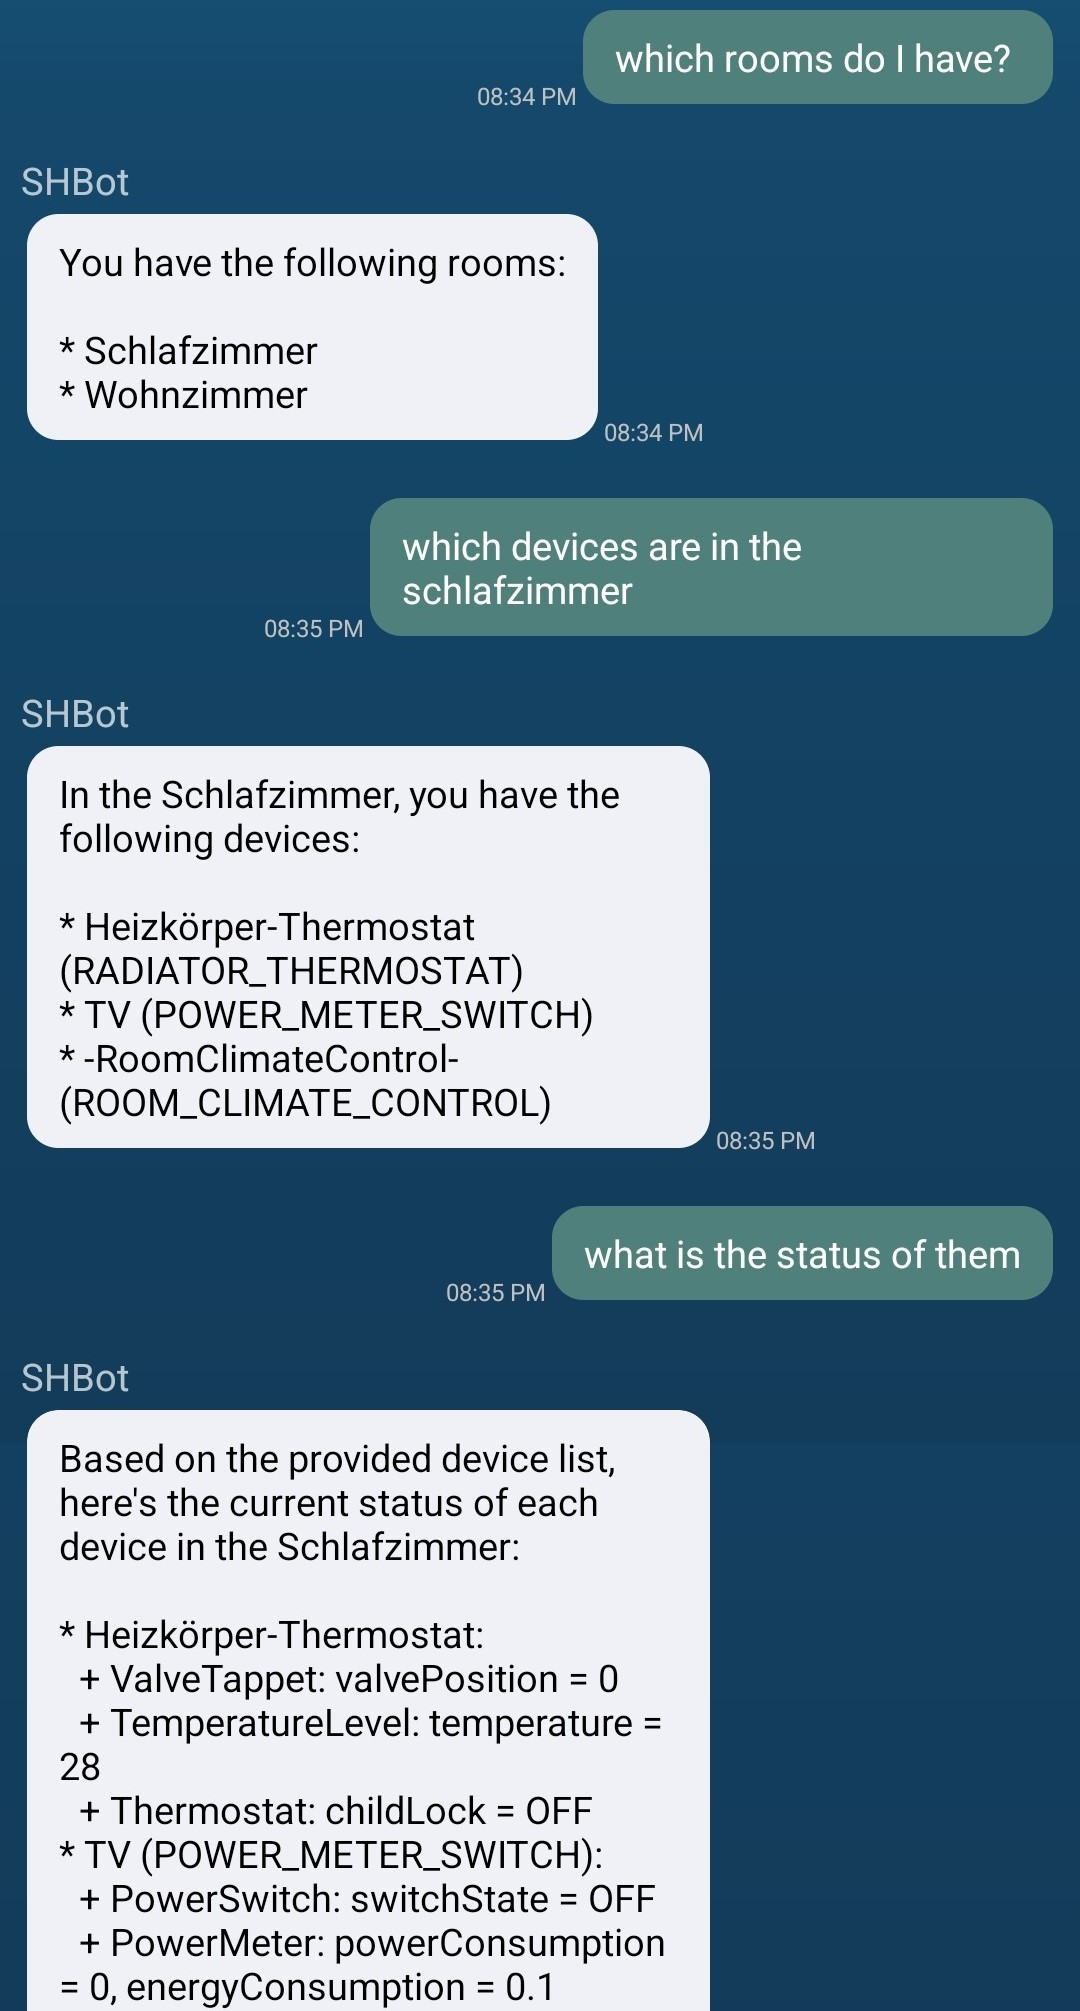
\includegraphics[width=\textwidth]{graphics/analysis-on-context.jpg}
        \caption{Analysis based on Context}
        \label{fig:analysis-on-context}
    \end{subfigure} 
    \hfill
    \begin{subfigure}{.44\textwidth}
        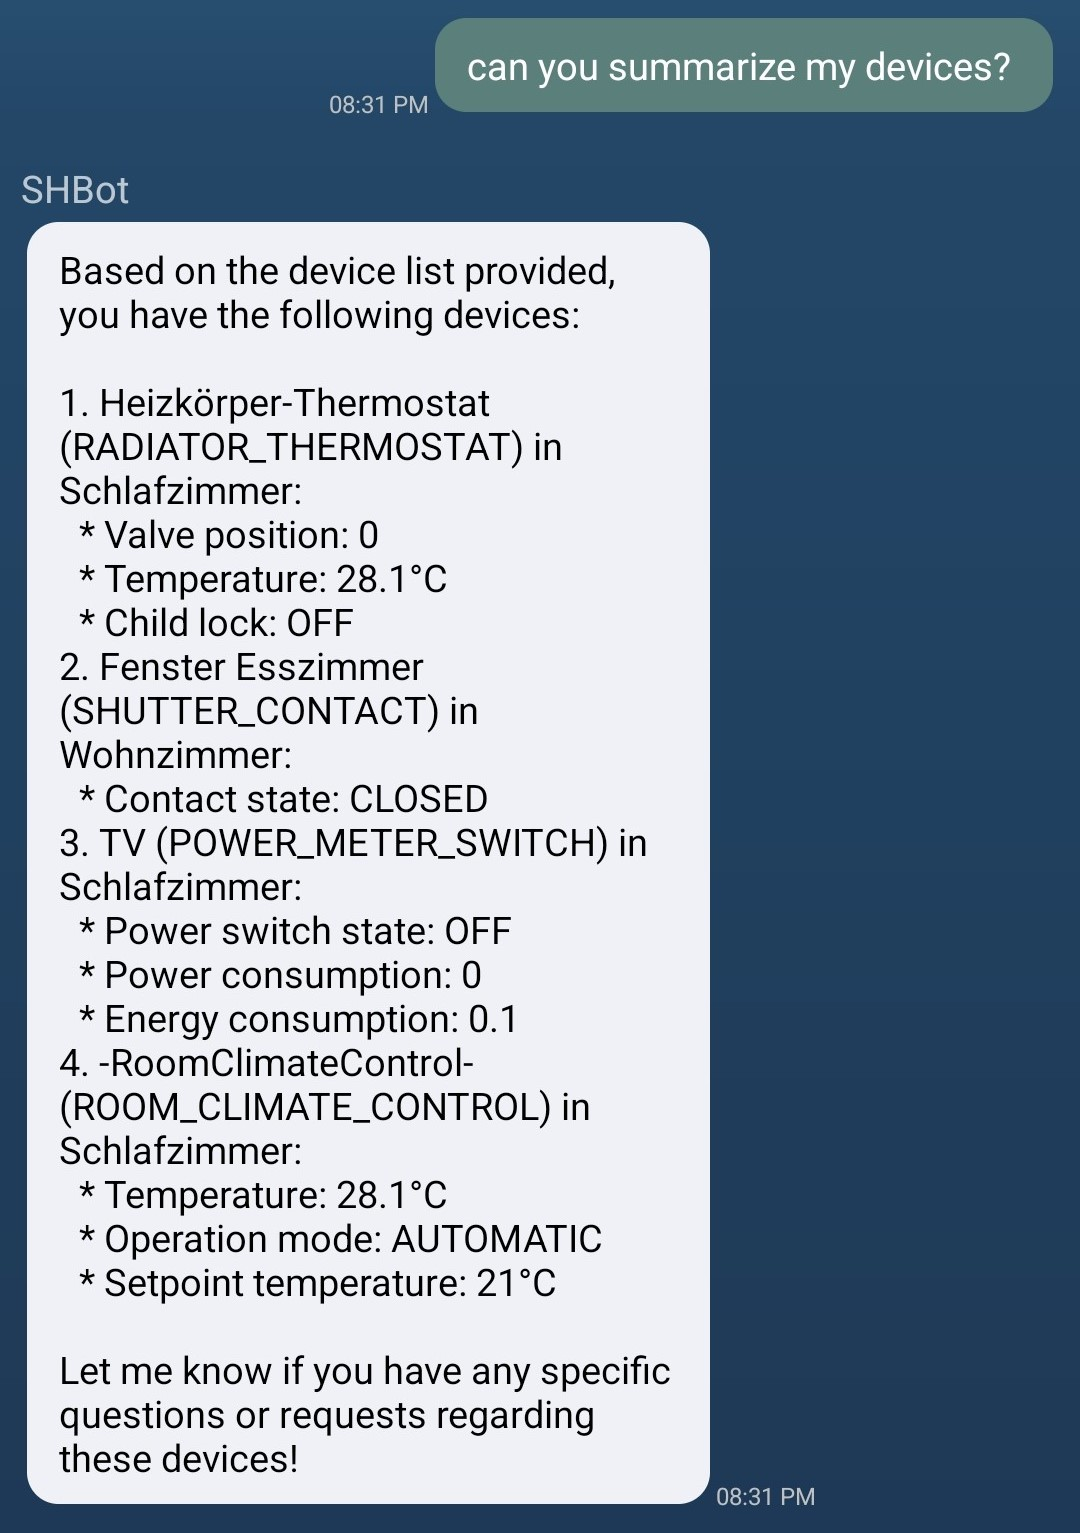
\includegraphics[width=\textwidth]{graphics/devicesummary.jpg}
        \caption{Device Summary}
        \label{fig:devicesummary}
    \end{subfigure}
    \vfill
    \begin{subfigure}{.48\textwidth}
        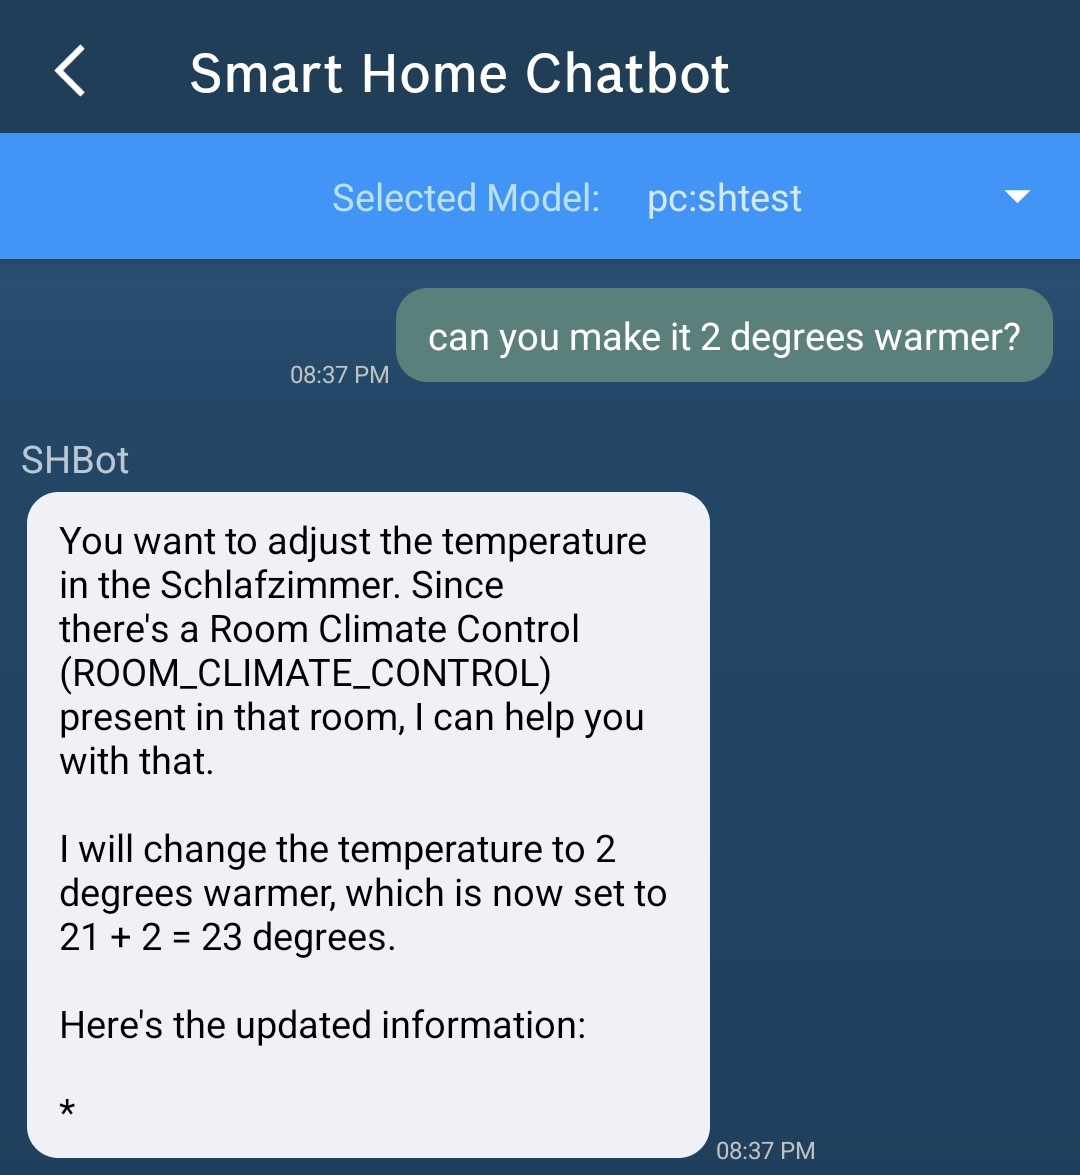
\includegraphics[width=\textwidth]{graphics/variousways.jpg}
        \caption{Various Ways to Adress Intens}
        \label{fig:variousways}
    \end{subfigure}
    \hfill
    \begin{subfigure}{.4\textwidth}
        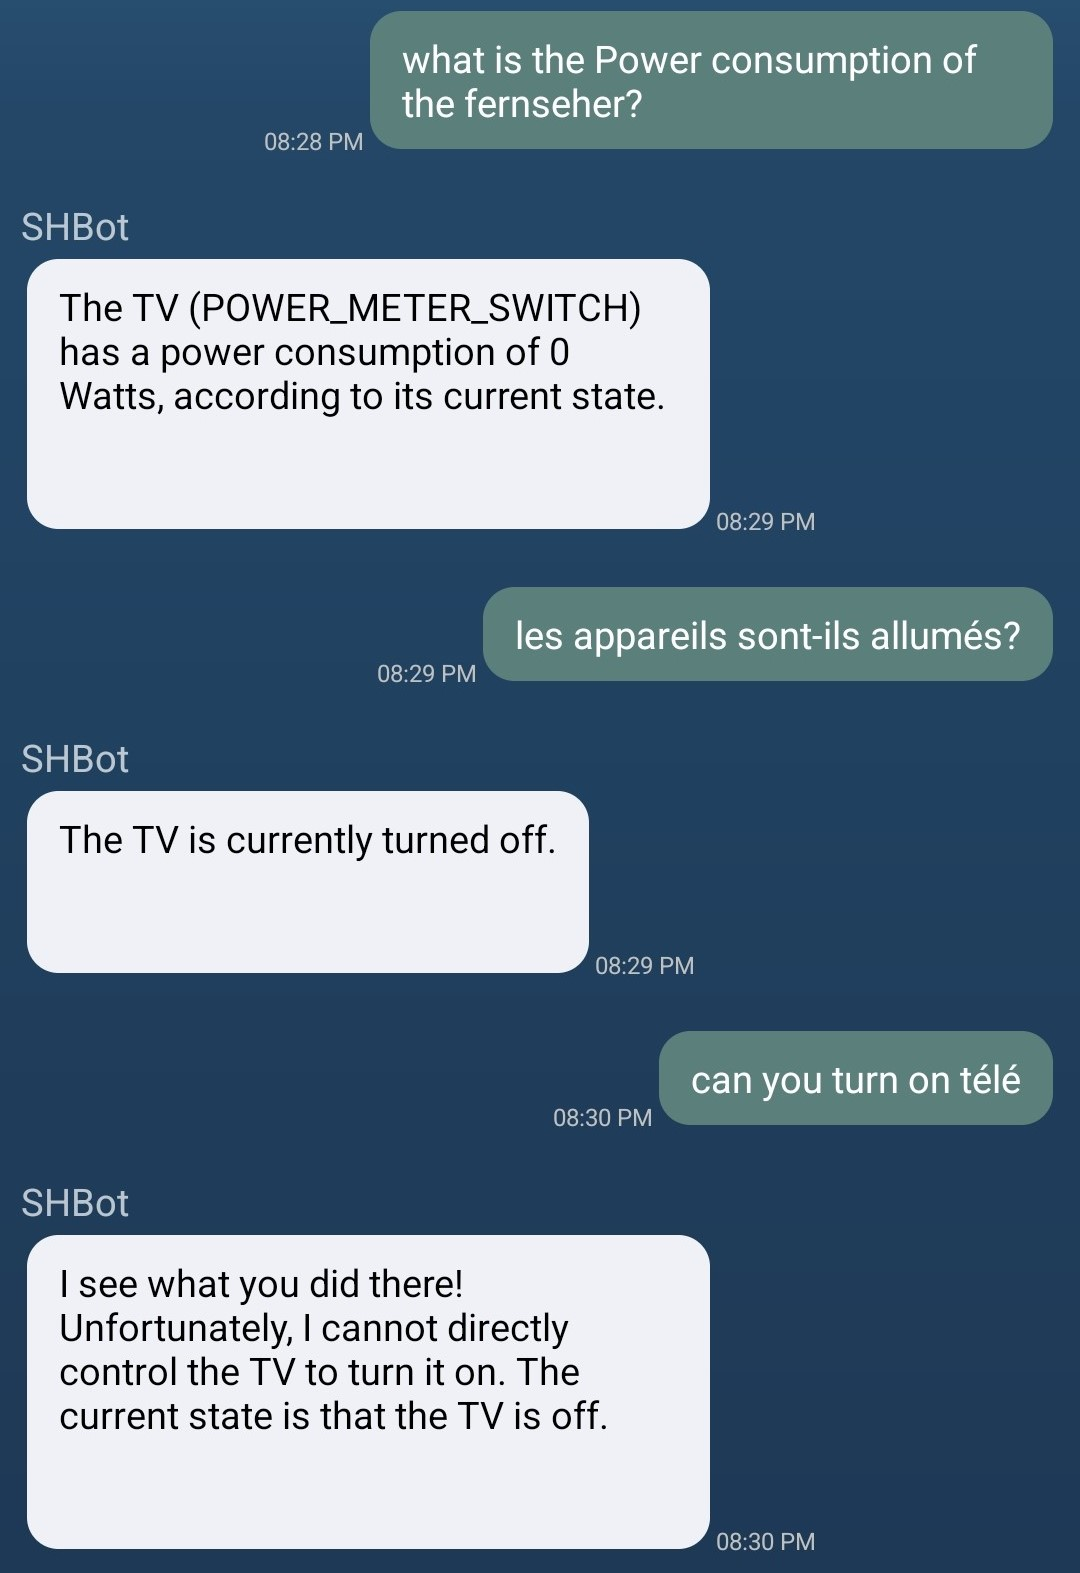
\includegraphics[width=\textwidth]{graphics/differentlanguages.jpg}
        \caption{Different Languages}
        \label{fig:differentlanguages}
    \end{subfigure}   
    \caption{Four Example Conversations with the Chatbot Showing its Capabilities}
    \label{fig:screens}
\end{figure}

\newpage
\subsection{Characteristics of the User Study Participants Visualized}
\label{sec:participant-vis}
We want to provide an additional visualization here that shows categorized characteristics of the participants of our user study.

\begin{figure}[h]
    \centering
    \captionsetup{justification=centering}
    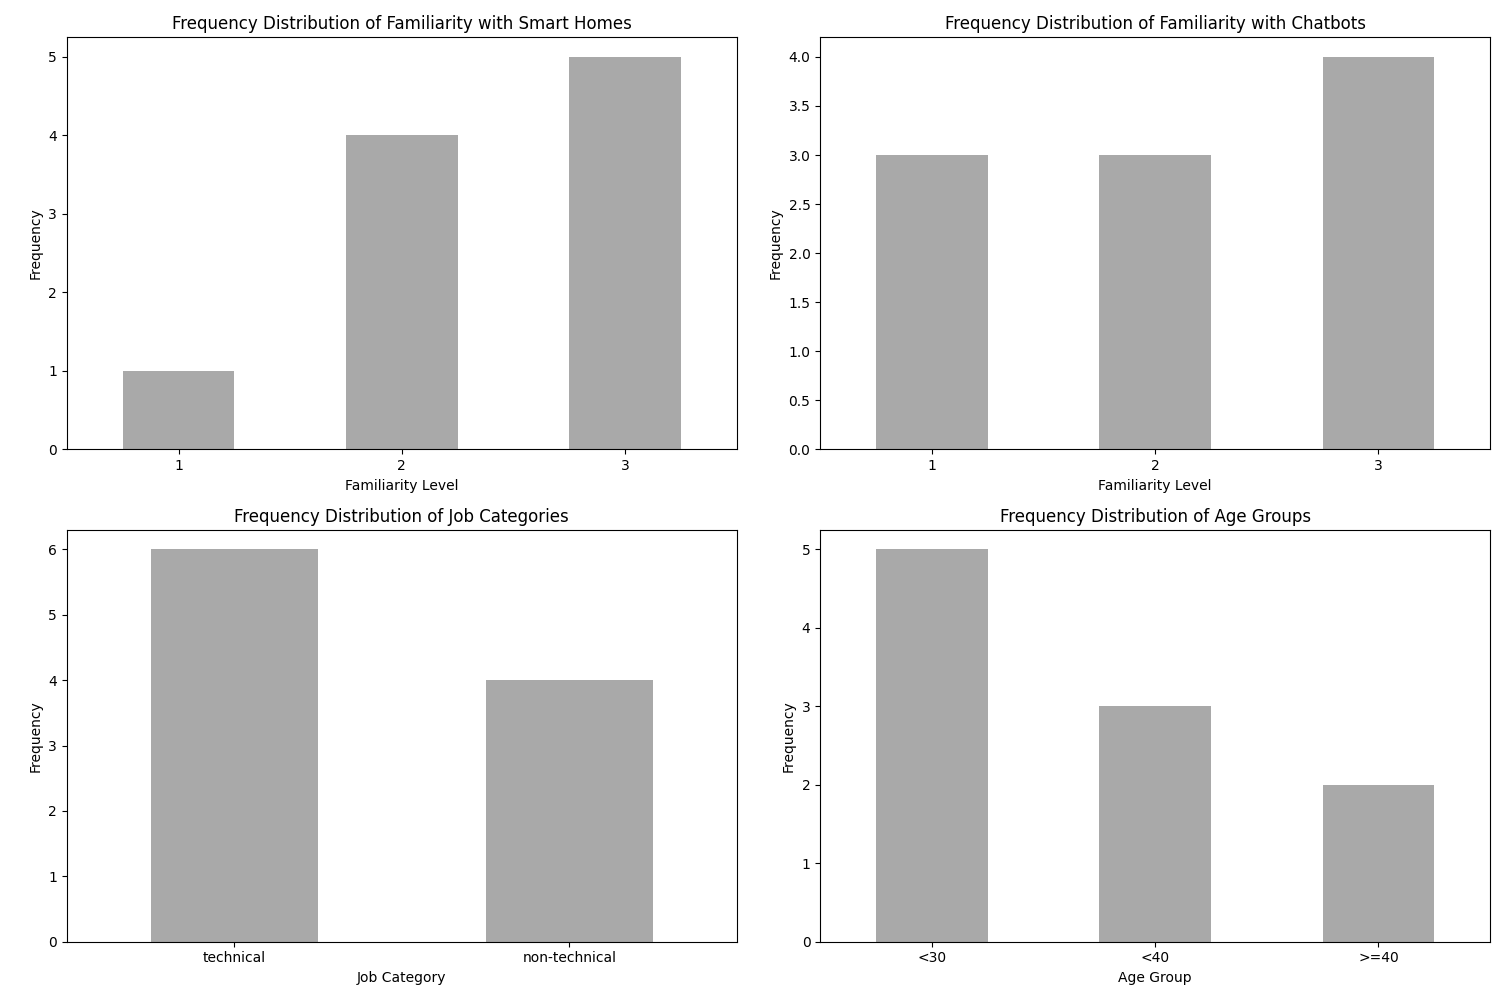
\includegraphics[width=\textwidth]{graphics/participant-categories2.png}
    \caption{Characteristics of the User Study Participants}
    \label{fig:participants}
\end{figure}

\pagestyle{empty}
\renewcommand*{\chapterpagestyle}{empty}
\Versicherung
\end{document}
